%%
%% Automatically generated file from DocOnce source
%% (https://github.com/hplgit/doconce/)
%%

% #define PREAMBLE

% #ifdef PREAMBLE
%-------------------- begin preamble ----------------------

% Style: Standard Springer svmono (book) - without courier font
\documentclass[graybox,envcountchap,sectrefs,final]{svmonodo}
%\pagestyle{headings}
\usepackage{mathptmx}
\usepackage{helvet}
\usepackage{lmodern}   % not svmono style, but gives prettier math symbols
%\usepackage{courier} % note: courier monospace font is too wide
\usepackage{type1cm}
\usepackage{framed}
\usepackage{booktabs}
\usepackage{subeqnarray}
\usepackage[bottom]{footmisc}
\usepackage{cite}
\usepackage{multicol}

\listfiles               %  print all files needed to compile this document

\usepackage{makeidx,color,setspace,amsmath,amsfonts,amssymb}
\usepackage[table]{xcolor}
\usepackage{bm}

\usepackage[pdftex]{graphicx}

% Packages for typesetting blocks of computer code
\usepackage{fancyvrb,framed,moreverb}

% Define colors
\definecolor{orange}{cmyk}{0,0.4,0.8,0.2}
\definecolor{tucorange}{rgb}{1.0,0.64,0}
\definecolor{darkorange}{rgb}{.71,0.21,0.01}
\definecolor{darkgreen}{rgb}{.12,.54,.11}
\definecolor{myteal}{rgb}{.26, .44, .56}
\definecolor{gray}{gray}{0.45}
\definecolor{mediumgray}{gray}{.8}
\definecolor{lightgray}{gray}{.95}
\definecolor{brown}{rgb}{0.54,0.27,0.07}
\definecolor{purple}{rgb}{0.5,0.0,0.5}
\definecolor{darkgray}{gray}{0.25}
\definecolor{darkblue}{rgb}{0,0.08,0.45}
\definecolor{darkblue2}{rgb}{0,0,0.8}
\definecolor{lightred}{rgb}{1.0,0.39,0.28}
\definecolor{lightgreen}{rgb}{0.48,0.99,0.0}
\definecolor{lightblue}{rgb}{0.53,0.81,0.92}
\definecolor{lightblue2}{rgb}{0.3,0.3,1.0}
\definecolor{lightpurple}{rgb}{0.87,0.63,0.87}
\definecolor{lightcyan}{rgb}{0.5,1.0,0.83}

\colorlet{comment_green}{green!50!black}
\colorlet{string_red}{red!60!black}
\colorlet{keyword_pink}{magenta!70!black}
\colorlet{indendifier_green}{green!70!white}

% Backgrounds for code
\definecolor{cbg_gray}{rgb}{.95, .95, .95}
\definecolor{bar_gray}{rgb}{.92, .92, .92}

\definecolor{cbg_yellowgray}{rgb}{.95, .95, .85}
\definecolor{bar_yellowgray}{rgb}{.95, .95, .65}

\colorlet{cbg_yellow2}{yellow!10}
\colorlet{bar_yellow2}{yellow!20}

\definecolor{cbg_yellow1}{rgb}{.98, .98, 0.8}
\definecolor{bar_yellow1}{rgb}{.98, .98, 0.4}

\definecolor{cbg_red1}{rgb}{1, 0.85, 0.85}
\definecolor{bar_red1}{rgb}{1, 0.75, 0.85}

\definecolor{cbg_blue1}{rgb}{0.87843, 0.95686, 1.0}
\definecolor{bar_blue1}{rgb}{0.7,     0.95686, 1}

\usepackage{listingsutf8}

% Common lstlisting parameters

\usepackage{calc}
\newlength{\lstboxwidth}  % width of lst box
\newlength{\framethickness}
\setlength{\framethickness}{0.5mm}
% for frame=trbl and a framerule that has significant size, set
% xleftmargin=5mm and xrightmargin=5mm.

\lstset{
  basicstyle=\small \ttfamily,
  breaklines=false,          % break/wrap lines
  breakatwhitespace=true,    % let linebreaks happen at whitespace
  breakindent=40pt,
  tab=,
  tabsize=4,                 % tab means 4 spaces
  %belowskip=\smallskipamount,  % space between code and text below
  xleftmargin=2mm,           % indentation of code frame
  xrightmargin=0mm,
  framexleftmargin=2mm,      % add frame space to the left of the code box
  %numbers=left,             % put line numbers on the left
  %stepnumber=2,             % stepnumber=1 numbers each line, =n every n lines
  framerule=\framethickness, % thickness of frame
  aboveskip=2ex,             % vertical space above code frame
  showstringspaces=false,    % show spaces in strings with an underscore
  showspaces=false,          % show spaces with an underscore
  showtabs=false,
  keepspaces=true,
  columns=fullflexible,      % tighter character kerning, like verb
  escapeinside={(*@}{@*)},   % (*@ \pause @*) in slides and math in code blocks
  extendedchars=\true,       % allows non-ascii chars, does not work with utf-8
}

% Internally defined styles for lstlisting

% Use this one without additional background color
\lstdefinestyle{blue1}{              % blue1 background for code snippets
backgroundcolor=\color{cbg_blue1},
}

% Use this one without additional background color
% (same as blue1, but with bar_blue1 frame)
\lstdefinestyle{blue1bar}{           % blue1 background for complete programs
backgroundcolor=\color{cbg_blue1},
frame=tb,                            % include frame
rulecolor=\color{bar_blue1},         % frame color
}

% Use this one without additional background color
\lstdefinestyle{gray}{
backgroundcolor=\color{cbg_gray},
%frame=tb,                            % include frame
%framerule=0.4pt                      % thickness of frame
rulecolor=\color{black!40},           % frame color
}

\lstdefinestyle{simple}{
commentstyle={},
}

% end of custom lstdefinestyles

\usepackage[T1]{fontenc}
%\usepackage[latin1]{inputenc}
\usepackage{ucs}
\usepackage[utf8x]{inputenc}

% Hyperlinks in PDF:

\usepackage{hyperref}
\hypersetup{
    breaklinks=true,
    colorlinks=true,
    linkcolor=black,
    urlcolor=black,
    citecolor=black,
    filecolor=black,
    %filecolor=blue,
    pdfmenubar=true,
    pdftoolbar=true,
    bookmarksdepth=3   % Uncomment (and tweak) for PDF bookmarks with more levels than the TOC
    }
%\hyperbaseurl{}   % hyperlinks are relative to this root

\setcounter{tocdepth}{3}  % levels in table of contents

\usepackage[framemethod=TikZ]{mdframed}

% --- begin definitions of admonition environments ---

% Admonition style "mdfbox" is an oval colored box based on mdframed
% "notice" admon
\definecolor{mdfbox_notice_background}{rgb}{1,1,1}
\newmdenv[
  skipabove=15pt,
  skipbelow=15pt,
  outerlinewidth=0,
  backgroundcolor=mdfbox_notice_background,
  linecolor=black,
  linewidth=2pt,       % frame thickness
  frametitlebackgroundcolor=mdfbox_notice_background,
  frametitlerule=true,
  frametitlefont=\normalfont\bfseries,
  shadow=false,        % frame shadow?
  shadowsize=11pt,
  leftmargin=0,
  rightmargin=0,
  roundcorner=5,
  needspace=0pt,
]{notice_mdfboxmdframed}

\newenvironment{notice_mdfboxadmon}[1][]{
\begin{notice_mdfboxmdframed}[frametitle=#1]
}
{
\end{notice_mdfboxmdframed}
}

% Admonition style "mdfbox" is an oval colored box based on mdframed
% "summary" admon
\definecolor{mdfbox_summary_background}{rgb}{1,1,1}
\newmdenv[
  skipabove=15pt,
  skipbelow=15pt,
  outerlinewidth=0,
  backgroundcolor=mdfbox_summary_background,
  linecolor=black,
  linewidth=2pt,       % frame thickness
  frametitlebackgroundcolor=mdfbox_summary_background,
  frametitlerule=true,
  frametitlefont=\normalfont\bfseries,
  shadow=false,        % frame shadow?
  shadowsize=11pt,
  leftmargin=0,
  rightmargin=0,
  roundcorner=5,
  needspace=0pt,
]{summary_mdfboxmdframed}

\newenvironment{summary_mdfboxadmon}[1][]{
\begin{summary_mdfboxmdframed}[frametitle=#1]
}
{
\end{summary_mdfboxmdframed}
}

% Admonition style "mdfbox" is an oval colored box based on mdframed
% "warning" admon
\definecolor{mdfbox_warning_background}{rgb}{1,1,1}
\newmdenv[
  skipabove=15pt,
  skipbelow=15pt,
  outerlinewidth=0,
  backgroundcolor=mdfbox_warning_background,
  linecolor=black,
  linewidth=2pt,       % frame thickness
  frametitlebackgroundcolor=mdfbox_warning_background,
  frametitlerule=true,
  frametitlefont=\normalfont\bfseries,
  shadow=false,        % frame shadow?
  shadowsize=11pt,
  leftmargin=0,
  rightmargin=0,
  roundcorner=5,
  needspace=0pt,
]{warning_mdfboxmdframed}

\newenvironment{warning_mdfboxadmon}[1][]{
\begin{warning_mdfboxmdframed}[frametitle=#1]
}
{
\end{warning_mdfboxmdframed}
}

% Admonition style "mdfbox" is an oval colored box based on mdframed
% "question" admon
\definecolor{mdfbox_question_background}{rgb}{1,1,1}
\newmdenv[
  skipabove=15pt,
  skipbelow=15pt,
  outerlinewidth=0,
  backgroundcolor=mdfbox_question_background,
  linecolor=black,
  linewidth=2pt,       % frame thickness
  frametitlebackgroundcolor=mdfbox_question_background,
  frametitlerule=true,
  frametitlefont=\normalfont\bfseries,
  shadow=false,        % frame shadow?
  shadowsize=11pt,
  leftmargin=0,
  rightmargin=0,
  roundcorner=5,
  needspace=0pt,
]{question_mdfboxmdframed}

\newenvironment{question_mdfboxadmon}[1][]{
\begin{question_mdfboxmdframed}[frametitle=#1]
}
{
\end{question_mdfboxmdframed}
}

% Admonition style "mdfbox" is an oval colored box based on mdframed
% "block" admon
\definecolor{mdfbox_block_background}{rgb}{1,1,1}
\newmdenv[
  skipabove=15pt,
  skipbelow=15pt,
  outerlinewidth=0,
  backgroundcolor=mdfbox_block_background,
  linecolor=black,
  linewidth=2pt,       % frame thickness
  frametitlebackgroundcolor=mdfbox_block_background,
  frametitlerule=true,
  frametitlefont=\normalfont\bfseries,
  shadow=false,        % frame shadow?
  shadowsize=11pt,
  leftmargin=0,
  rightmargin=0,
  roundcorner=5,
  needspace=0pt,
]{block_mdfboxmdframed}

\newenvironment{block_mdfboxadmon}[1][]{
\begin{block_mdfboxmdframed}[frametitle=#1]
}
{
\end{block_mdfboxmdframed}
}

% --- end of definitions of admonition environments ---

% prevent orhpans and widows
\clubpenalty = 10000
\widowpenalty = 10000

\newenvironment{doconceexercise}{}{}
\newcounter{doconceexercisecounter}

% Let exercises, problems, and projects be numbered per chapter:
\usepackage{chngcntr}
\counterwithin{doconceexercisecounter}{chapter}


% ------ header in subexercises ------
%\newcommand{\subex}[1]{\paragraph{#1}}
%\newcommand{\subex}[1]{\par\vspace{1.7mm}\noindent{\bf #1}\ \ }
\makeatletter
% 1.5ex is the spacing above the header, 0.5em the spacing after subex title
\newcommand\subex{\@startsection{paragraph}{4}{\z@}%
                  {1.5ex\@plus1ex \@minus.2ex}%
                  {-0.5em}%
                  {\normalfont\normalsize\bfseries}}
\makeatother


% Redefine double page clear to make it a blank page without headers
% (from BYUTextbook)
\makeatletter
\def\cleardoublepage{\clearpage\if@twoside \ifodd\c@page\else
\hbox{}
\thispagestyle{empty}
\newpage
\if@twocolumn\hbox{}\newpage\fi\fi\fi}
\makeatother
% These commands fiddle with the space left for page numbers in the TOC
% (from BYUTextbook)
\makeatletter
%\renewcommand{\@pnumwidth}{2em}
%\renewcommand{\@tocrmarg}{2.85em}
\makeatother

% --- end of standard preamble for documents ---


% insert custom LaTeX commands...

\raggedbottom
\makeindex
\usepackage[totoc]{idxlayout}   % for index in the toc
\usepackage[nottoc]{tocbibind}  % for references/bibliography in the toc

%-------------------- end preamble ----------------------

\begin{document}

% matching end for #ifdef PREAMBLE
% #endif

\newcommand{\exercisesection}[1]{\subsection*{#1}}

% This file is to be run by preprocess to produce newcommands.tex
% to be included in .tex files.
% There are format-specific tests here for the newcommands (i.e.,
% different definitions of the commands depending on latex or mathjax).

% Newcommands for LaTeX math.
\newcommand{\tp}{\thinspace .}
\newcommand{\dx}{\thinspace dx}
\newcommand{\ds}{\thinspace ds}
\renewcommand{\Re}{\bbbr}
\newcommand{\Oof}[1]{\mathcal{O}(#1)}
\newcommand{\Prob}[1]{\hbox{P}(#1)}
\newcommand{\Var}[1]{\hbox{Var}(#1)}
\newcommand{\Cov}[2]{\hbox{Cov}(#1,#2)}
\newcommand{\StDev}[1]{\hbox{StDev}(#1)}

\newcommand{\F}{\mathbf{F}}
\newcommand{\f}{\mathbf{f}}
\newcommand{\bfx}{\mathbf{x}}
\newcommand{\bfX}{\mathbf{X}}
\newcommand{\bfu}{\mathbf{u}}
\newcommand{\bfP}{\mathbf{P}}
\newcommand{\bfS}{\mathbf{S}}
\newcommand{\bfE}{\mathbf{E}}
\newcommand{\C}{\mathbf{C}}
\newcommand{\stress}{\mathbf{\sigma}}
\newcommand{\strain}{\mathbf{\epsilon}}
\newcommand{\bfr}{\mathbf{r}}
\newcommand{\bfv}{\mathbf{v}}
\newcommand{\bfa}{\mathbf{a}}
\newcommand{\bfA}{\mathbf{A}}
\newcommand{\U} {\mathbf{U}}
\newcommand{\R} {\mathbf{R}}
\newcommand{\n}{\mathbf{n}}
\newcommand{\N}{\mathbf{N}}
\newcommand{\T}{\mathbf{T}}
\newcommand{\bfs}{\mathbf{s}}
\newcommand{\bfI}{\mathbf{I}}
\newcommand{\bphi}{\mathbf{\phi}}
\newcommand{\modvec}[1]{\mathbf{#1}}
\newcommand{\modten}[1]{\mathbf{#1}}




\newcommand{\beq}{\begin{equation}}
\newcommand{\eeq}{\end{equation}}



% Use footnotesize in subscripts
\newcommand{\subsc}[2]{#1_{\mbox{\footnotesize #2}}}




% ------------------- main content ----------------------

% Note on the Springer T4 style: here we use the modifications
% introduced in t4do.sty and svmonodo.sty (both are bundled with DocOnce).


\frontmatter
\setcounter{page}{3}
\pagestyle{headings}


% ----------------- title -------------------------

\title{Introduction to scientific programming with Python}

% ----------------- author(s) -------------------------

\author{Joakim Sundnes\footnote{Simula Research Laboratory and Department of Informatics, University of Oslo.}}

% ----------------- end author(s) -------------------------

\date{Feb 21, 2020}
\maketitle

% !split
\chapter*{Preface}
\addcontentsline{toc}{chapter}{Preface}
\label{ch:preface}

These lecture notes are based on the book "A Primer on Scientific Programming with Python"
by Hans Petter langtangen. The notes are meant to be used as a supplement to the book, and
are intentionally written in a brief and compact style. If you want a more detailed explanation
of some concept, or are curious about some details or how various Python programming concepts are
used in practice, the book is an excellent resource. The book and these notes are written specifically
for the course IN1900, and they follow the same teaching philosophy and general structure. The overarching idea
is that the only way to learn to program is to program. Reading theory is useful, but without actual programming
practice the value is very limited. Following this idea, the typical workflow in IN1900 is the following:

\begin{enumerate}
 \item Briefly introduce a new programming concept

 \item Illustrate its use through a few relevant examples

 \item Train the new concept through a number of programming exercises
\end{enumerate}

\noindent
The target audience for these notes is people with no background in programming. The notes cover the
Python language, but also introduces and explains fundamental constructs such as loops, functions and lists,
which are generic and relevant for all programming langugages. For experienced programmers that are new
to Python the notes can be used as a quick reference for learning syntax and basic Python-specific
functionality, but other books may be more suitable for this group.

From the doconce book setup:
\begin{enumerate}
\item Chapters can exist as stand-alone documents in different formats:
\begin{itemize}

   \item traditional LaTeX-style PDF report,

   \item web pages with various fancy stylings (e.g., Sphinx, Bootstrap)
     and possibility for multi-media elements,

   \item IPython notebooks,

   \item blog posts (not exemplified here, but \href{{http://hplgit.github.io/doconce/doc/pub/manual/html/manual.html#blog-posts}}{straightforward}\footnote{\texttt{http://hplgit.github.io/doconce/doc/pub/manual/html/manual.html\#blog-posts}}),

   \item wiki (if you do not need mathematical typesetting).

\end{itemize}

\noindent
\item Chapters can be flexibly assembled into a traditional LaTeX-based
   PDF book for a traditional publisher, or a fancy ebook.

\item The book and the individual chapter documents may have different
   layouts.

\item Active use of preprocessors (Preprocess and Mako) makes it
   easy to have different versions of the chapters,
   e.g., a specialized version for a course and
   a general version for the world book market).

\item DocOnce has support for important elements in teaching material:
   eye-catching boxes (admonitions), quizzes, interactive code,
   videos, structured exercises, quotes.

\item Study guides or slides can easily be developed from the running
   text and stored along with the chapters. These can be published
   as {\LaTeX} Beamer slides, reveal.js slides, and IPython notebooks.
\end{enumerate}

\noindent
These features have the great advantage that a book can evolve from
small documents, thereby making the barrier for book writing much smaller.
Also, several appealing ebook formats can be produced, both for the
book and the individual chapter documents. The chances that your students
read a chapter on the bus becomes larger if the chapter is available
as attractive, screen-fit Bootstrap pages on the smart phone than if you
just offer the classic {\LaTeX} PDF which actually requires a big screen or a
printer.

Implementation of point 1 and 2 is not trivial and requires some rules
that might not feel natural at first sight in the setup.  Writing a
book soon becomes a technically and mentally complex task, just like
developing a software system. For the latter people have invented a
lot of sophisticated technologies and best practices to deal with the
complexity. The present setup for books is a similar collection of my
own technologies and best practices, developed from writing
thousands of pages. In particular, the setup has been successfully
used for the large-scale 900-page Springer book ``A Primer on
Scientific Programming with Python'' \cite{Langtangen_2014} (individual
chapters of this book, e.g.~\cite{Langtangen_TCSE6_looplist}, can be
examined online in various ebook formats) as well as for
\href{{http://hplgit.github.io/num-methods-for-PDEs/doc/pub/index.html}}{books in the works}\footnote{\texttt{http://hplgit.github.io/num-methods-for-PDEs/doc/pub/index.html}}.

To use this setup, just clone the \href{{https://github.com/hplgit/setup4book-doconce}}{repository}\footnote{\texttt{https://github.com/hplgit/setup4book-doconce}} and you have the
directory structure, the scripts, and example files to get started with
a book project at
once! The source files for this book (especially in
\texttt{doc/src/chapters/rules}) constitute nice demonstrations for learning
about basic and advanced DocOnce writing techniques.



\vspace{3mm}




\vspace{3mm}




\vspace{3mm}




\vspace{3mm}



\noindent
{\it April 2015}  \hfill  {\it Hans Petter Langtangen}



\tableofcontents


\vspace{1cm} % after toc

\mainmatter




% !split
\chapter{Introduction}
\label{ch:intro}

This course teaches the Python language, which has a number of advantages as a first programming language, but also
some minor drawbacks. The main advantage of Python is that it is a so-called "high-level" language, with simple and
intuitive syntax that makes it easy to get started. However, although it is suitable as a beginner's language, Python is also
suitable for more advanced tasks, and is currently one of the most widely used programming languages worldwide.

One of the more important drawbacks of Python is tightly linked to its main advantages. Being a flexible high-level
language, writing small programs can be very quick, but the code can easily get messy when writing something bigger.
Other languages like C, C++ and Java enforces more structure in the code, which is annoying when you want to write
a small program quickly, but may be efficient in the long run when writing larger programs. However, it is
certainly possible to write neat and nicely structured programs in Python as well, but this requires
a choice of the programmer to follow certain principles of coding style, and is not forced by the language itself.
We will comment more on coding style later in these notes.

Another slightly annoying aspect of Python is that it exists in different versions. At the time of writing this
(August 2019), Python 3 is dominant, with the newest stable version being Python 3.7.
All the examples in these notes are in Python 3, but the latest version of
"A Primer on Scientific Programming with Python" was published in 2016 and is still Python 2. For the topics covered
here the difference between the two version are very small, and combining the notes with the book should not
cause much trouble. The most significant difference, which we will run into very early, is a difference in
the command \texttt{print} which we use to write text and numbers to the screen. We will comment more on this and some
other differences later.

Finally, a nice feature of Python is that it can be used in many different ways. This is very
useful for a number of purposes, but can be confusing in the beginning. Here's a quick overview of how
we use Python in IN1900:

\begin{itemize}
  \item Writing regular programs using a text editor or an IDE (Integrated development environment) is the
    "classical" way of programming, and will be the most widely used in the course. One writes small programs using a
    text editor, stores them in a file, and runs them from a terminal window with a command such as \Verb!python my_program.py!.
    All exercises in IN1900 are to be handed in as ".py"-files, so this way of programming will probably be
    your main style of working through the course. If one prefers an IDE, a convenient choice is Spyder, which
    is installed automatically if installing Python from Anaconda. See the IN1900 course website for more information.

  \item Python can be used interactively in the terminal, by typing \texttt{python} or \texttt{ipython} in a terminal window,
    without a subsequent file name. This will open an environment for typing and running Python commands, which is not very
    suitable for writing programs over several lines, but extremely useful for testing Python commands
    and statements, or simply
    using Python as a calculator. The two versions \texttt{python} and \texttt{ipython} work largely the same way, but \texttt{ipython} has a
    number of additional features and is recommended. An \texttt{ipython} window can also be started for instance
    from the \emph{Anaconda navigator}, which is convenient on Windows.

  \item \emph{Jupyter notebooks} are a form of interactive notebooks that combine code and text. These are read viewed a
    browser and look quite similar to a simple web page, but an important difference is that the code segments are "live"
    Python code that can be run, changed and re-run while reading the document. These notes are available as Jupyter
    notebooks, and most of the slides used in the lectures will also be in this format.
\end{itemize}

\noindent
For more detailed instructions on how to install and run Python on various platforms we refer to the course web site.

\subsection{The first example; Hello world!}
Most introductory books on programming start with a so-called "Hello world!"-program, which is a program
that simply writes the words "Hello world!" to the screen. In Python, this program is just a single line;
\begin{lstlisting}[language=Python,style=blue1bar]
print("Hello world!")
\end{lstlisting}
To write and run such a program, open your favourite editor (Atom, gedit, Emacs etc.) type
the given line and save the file with a suitable filename, for instance \texttt{hello.py}. Then, open a terminal or an iPython window,
navigate to the directory where you saved the file (\texttt{cd} and \texttt{ls} are the essential commands, see the course web site for a
quick guide). The type \texttt{python hello.py} in the terminal, or \texttt{run hello.py} if you are using iPython. The output appears
in the terminal right after the command. If you are using an IDE, this is essentially an editor and an iPython/terminal window
combined. For instance, in the Spyder IDE the editor is in the upper left window, and you type the program and save the file there.
The, the window in the lower right corner is the iPython window where you run the program.

While the "Helllo world!"-program may seem like a silly example, it actually serves a number of useful purposes. First of all,
running this small program will verify that you have installed Python properly, and that you have installed the right version.
It also introduces the function \texttt{print}, which will be used virtually every time we program, and
illustrates how we use quotes to define a \texttt{string} in Python. While \texttt{print} is a word that Python understands, \emph{hello} and
\emph{world} are not. By using the quotes we tell Python that it should not try to understand (or interprete) these words, but
rather treat it as a simple text that in this case is to be printed to the screen. More about this later. Furthermore, this simple example
illustrates the most frequently encountered difference between Python versions 2 and 3. In Python 2, the program would read
\texttt{print "Hello world"}, i.e.~without the parantheses. The examples in the book by Langtangen, which are written
in Python 2, will stop with an error message if you try to run them using Python 3. In most cases the only error is the
missing parantheses, which is usually indicated by the error message, and adding parantheses to all the print statements
will make most of the examples run fine in Python 3.

The tiny "Hello world!" example is also a good candidate for testing the interactive Python shell mentioned above.
In a regular terminal window on Mac or Linux, the example would look something like this:
\begin{lstlisting}[language=Python,style=blue1]
Terminal> python
Python 3.7.3 (default, Mar 27 2019, 16:54:48)
[Clang 4.0.1 (tags/RELEASE_401/final)] :: Anaconda, Inc. on darwin
Type "help", "copyright", "credits" or "license" for more information.
>>> print("Hello world!")
Hello world!
>>>
\end{lstlisting}
As mentioned above, the interactive shell is very useful for testing and learning how various Python functions are used, and for using
Python as a calculator. 
% !split
\chapter{Computing with formulas}
\label{ch:formulas}
% TITLE: Ch.1: Programming with formulas
% AUTHOR: Joakim Sundnes at Simula Research Laboratory {\&} University of Oslo, Dept.~of Informatics
% DATE: Feb 21, 2020




\section{Programming mathematical formulas}
In this chapter we will take one step beyond the "Hello world!"-example, and introduce programming
with mathematical formulae. Such formulae are essential parts of most programs written for scientific applications,
as well as a number of other applications, and they are also useful for introducing several fundamental concepts
in programming. After working through the examples in this chapter you will:
\begin{itemize}
 \item Be able to use Python's \texttt{print} function to output text and numbers

 \item Know what \emph{variables} are, and how they are used in programs

 \item Know how to program mathematical expressions in Python

 \item Know about \emph{types}, and how you can check the type of a variable

 \item Be able to use \emph{comments} to make your programs more readable
\end{itemize}

\noindent
To introduce these concepts, consider first a
formula from high school physics, describing the height of a ball in vertical motion
\[ y(t) = v_0t- \frac{1}{2}gt^2 \]
where
\begin{itemize}
  \item $y$ is the height (position) as function of time $t$

  \item $v_0$ is the initial velocity at $t=0$

  \item $g$ is the acceleration of gravity
\end{itemize}

\noindent
The task is now to write a program that computes $y$ for given values of $v_0$, $g$ and $t$. We could of course easily do
this with a calculator, but a small program is much more flexible and powerful. To evaluate the formula above,
we first need to assign some values to $v_0$, $g$ and $t$, and then make the calculation. Choosing for instance
$t=0.6, g = 9.81$, and $v_0=5$, a complete Python program for evaluating the formula above reads
\begin{lstlisting}[language=Python,style=blue1bar]
print(5*0.6 - 0.5*9.81*0.6**2)
\end{lstlisting}
As for the example above, this line can be typed into an interactive Python session, or written in an editor and stored in a file, for instance
\texttt{ball1.py}. Then, the program is run with \texttt{python ball1.py} in a regular terminal, or \texttt{run ball1.py} in an iPython window or  Spyder.

The \texttt{ball1.py}-program is not much more complex, or more useful, than the "Hello world!"-example above, but notice that in this case
we did not use quotation marks inside the parantheses. The reason is that we actually want Python to evaluate the formula,
and print the result to the screen, which works fine as long as the text inside the paranthesis is valid Python code. If we
put quotation marks around the formula above, the code would still work, but the result is not what we want (try it!).
At this point it is also worth noting that while Python may be a "flexible" and "high-level" language, as described above,
all programming languages are extremely pick about spelling and grammar. Consider for instance the line
\begin{lstlisting}[language=Python,style=blue1]
write(5*0,6 - 0,5*9,81*0,6^2)
\end{lstlisting}
While most people may read this line quite easily, and interpret it as the physics formula above, it makes no sense
as a Python program. There are multiple errors: \texttt{write} is not a legal Python word in this context, comma has another
meaning than in math, and the hat does not mean exponentiation. We have to be extremely accurate with how we write
computer programs, and it takes time and experience to learn this.


The evaluation of the mathematical formula above is performed according to the standard rules. The terms are evaluated one by
one, starting from left, exponentiation is performed first and then multiplication and division. If we want to control the
order of evaluation, we can use parantheses, just as we would do in mathematics. For instance these two lines here will
provide quite different results:
\begin{lstlisting}[language=Python,style=blue1bar]
print(2 + 2*3)
print((2 + 2)*3)
\end{lstlisting}
\begin{lstlisting}[language=Python,style=gray]
8
12
\end{lstlisting}
The use of parantheses to group calculations works exactly as in mathematics, and is not very difficult to understand for people with
a mathematical background. However, when programming more complicated formulas it is very easy to make mistakes such as forgetting or misplacing
a closing paranthesis. This mistake is probably the most common source of error when programming mathematical formulas, and even for
experienced programmers it is worth paying close attention to the order and number of parantheses in the expressions. Getting it wrong will
either lead to an error message when the code is run or to a program that runs
fine but gives an unexpected results. The first type of error is usually quite easy to find and to fix, but the latter may be much harder.

Although Python is quite strict on the spelling and grammar, or \emph{syntax}, of the formulas, there is some flexibility. For instance,
whitespace, or blanks, inside a formula does not matter at all. An expression like \texttt{5    *2} works just as well as \texttt{5*2}. In general, whitespace
in a Python program only matters if it is at the start of a line, which we will come back to later. Otherwise, one should use whitespace
in order to make the code as readable as possible to humans, since Python will ignore it anyway.


\subsection{Store numbers in variables to make a program more readable}

In mathematics we are used to variables, such as $v_0$, $g$ and $t$ in the formula above. We can use variables in a
program to, which makes the program easier to read and understand:
\begin{lstlisting}[language=Python,style=blue1]
v0 = 5
g = 9.81
t = 0.6
y = v0*t - 0.5*g*t**2
print(y)
\end{lstlisting}
\begin{lstlisting}[language=Python,style=gray]
1.2342
\end{lstlisting}
This program spans several lines of text and uses variables, but otherwise performs the same calculations
and gives the same output as the one-line program above. Even for this very simple example the use of
variables has a few advantages, mainly that the program becomes easier to read, the physics formula
is much more recognizable, and changing the value of a given variable is easier. The latter point is true in
particular for the variable \texttt{t}, which occurs twice in the formula. To evaluate the formula at a new time point,
we now only need to assign a new value to the variable in one place, while the one-line version of the program has to be
changed in two places. The latter is very error prone, since it is easy to forget one of the places that needs to be changed,
and should always be avoided. If the same number occurs more than once in a program, you should always use a
variable to store it.

The instructions in the program are called \emph{statements}, and are executed one by one when we run the program.
It is common to have one statement per line, although it is possible to put muleiple statements on one line,
separated by semicolon, as in \texttt{v0 = 5; g = 9.81; t = 0.6}.
For people new to programming, especially those
used to reading mathematics, it is worth taking note of
the strict sequence in which the lines are executed. In the mathematical equation above we first introduced a formula with
some variables ($v_0, g, t$), and then defined these variables further down. This approach is completely standard
in mathematics, but it makes no sense in programming. Programs are executed line by line from the top, so all definitions of
variables must be done \emph{above} the line where they are used.

Choosing variable names is up to the programmer, and in general there is great flexibility in choosing such names.
In mathematics it is common to use a single letter for a variable, but a variable in Python program can be any
word containing the letters a-z, A-Z, underscore \Verb!_! and the digits 0-9, but it cannot start with a digit. Variable names
Python are also case-sensitive, for instance \texttt{a} is different from \texttt{A}. The following program is identical to the
one above, but with different variable names:
\begin{lstlisting}[language=Python,style=blue1bar]
initial_velocity = 5
accel_of_gravity = 9.81
TIME = 0.6
VerticalPositionOfBall = initial_velocity*TIME - \ 
                         0.5*accel_of_gravity*TIME**2
print(VerticalPositionOfBall)
\end{lstlisting}
\begin{lstlisting}[language=Python,style=gray]
1.2342
\end{lstlisting}
Note that the backslash allows an expression to be continued on the next line. These alternative names are arguably
more descriptive, but also makes the formula very long and cumbersome to read. Choosing good variable names is often a
balance of being descriptive and being short and compact, and can be quite important for making a program easy to
read and understand. Writing readable and understandable code also makes it easier to find errors in the code, so
choosing good variable names is worthwhile even if you are the only person who will ever read your code. Although the
choice of variable names is up to the programmer, some names are reserved in Python and are not allowed to be used. These are \texttt{and},
\texttt{as},
\texttt{assert},
\texttt{break},
\texttt{class},
\texttt{continue},
\texttt{def},
\texttt{del},
\texttt{elif},
\texttt{else},
\texttt{except},
\texttt{exec},
\texttt{finally},
\texttt{for},
\texttt{from},
\texttt{global},
\texttt{if},
\texttt{import},
\texttt{in},
\texttt{is},
\texttt{lambda},
\texttt{not},
\texttt{or},
\texttt{pass},
\texttt{print},
\texttt{raise},
\texttt{return},
\texttt{try},
\texttt{with},
\texttt{while}, and
\texttt{yield}.
This list is difficult to memorize at this point, but we will use many of these words in our programs later so it will be
quite natural that they cannot be used as variable names. However, it may be worth taking note of \texttt{lambda}, since the Greek
letter $\lambda$ is commonly used in mathematical formulas. Since
Python does not understand Greek letters it is common to just spell them out when programming a formula, i.e.~$\alpha$ becomes \texttt{alpha} etc.,
but for $\lambda$ we will need to introduce a small intentional typo and write \texttt{lmbda} or similar.

The program above contains two different types of statements; several assignment statements, which assign values to variables,
followed by a single print statement at the end. It may be quite intuitive how these statements work, but the assignment statements
are worth looking into in more detail. In these statements, the right hand side of the equality sign is evaluated first, and then
the result is assigned to the variable on the left. An effect of this execution order is that statements like the following work just
fine, and are common to see in programs:
\begin{lstlisting}[language=Python,style=blue1]
t = 0.6
t = t + 0.1
print(t)
\end{lstlisting}
\begin{lstlisting}[language=Python,style=gray]
0.7
\end{lstlisting}
The second line of this code does not make sense as a mathematical equation, but is a perfectly valid assignment in a computer
program. The right hand side is
evaluated first, using the value of \texttt{t} already defined, and then \texttt{t} is updated to the result of the calculation. The
equality sign in Python is called the \emph{assignment operator}, and it works almost like an equality sign in mathematics, but not quite.
If, for instance, we want to compare two numbers to figure out if they are equal, the operator to use in Python is \texttt{==}. For instance,
a trivial comparison may look like
\begin{lstlisting}[language=Python,style=blue1]
a = 5
print(a == 5)
\end{lstlisting}
\begin{lstlisting}[language=Python,style=gray]
True
\end{lstlisting}
We will see many more such examples later.

\subsection{Comments are useful to explain how you think in programs}
We may combine the strengths of the two programs above, and have both compact variable names \emph{and} a
more detailed description of what they are. This can be done using \emph{comments}, as illustrated in the
following example:
\begin{lstlisting}[language=Python,style=blue1]
# program for computing the height of a ball
# in vertical motion
v0 = 5    # initial velocity
g = 9.81  # acceleration of gravity
t = 0.6   # time
y = v0*t - 0.5*g*t**2  # vertical position
print(y)
\end{lstlisting}
\begin{lstlisting}[language=Python,style=gray]
1.2342
\end{lstlisting}
In this code all the text following the \Verb!#! symbol is treated as a comment, and effectively ignored by Python.
Comments are used to explain what the computer instructions mean, what variables mean, how the
programmer reasoned when the program was written, etc. Comments can be very useful for increasing readability,
although they should not be over-used. Comments that say no more than the code, for instance \Verb!a = 5  # set a to 5!,
are not very useful.

\subsection{Variables have different \emph{types}}

So far all the variables we have used have been numbers, which is also what we are used to from mathematics. However, in
a computer program we can have many different kinds of variables, not just numbers. All variables have a \emph{type}, which is
usually decided automatically based on the value we assign to it. For instance, the statement \texttt{v0 = 5} will create
a variable of the type \emph{integer}, or \texttt{int}, while for instance \texttt{t = 0.6} will create a variable of type \texttt{float}, representing
a floating point number. We can also have text variables, called strings in Python, having type \texttt{str},
for string. For instance, the "Hello world!"-example above could have been written as
\begin{lstlisting}[language=Python,style=blue1]
hello = "Hello world!"
print(hello)
\end{lstlisting}
\begin{lstlisting}[language=Python,style=gray]
Hello world!
\end{lstlisting}
We will encounter many more variable types in subsequent chapters. The type of a variable
decides how it can be used, and also the effect of various operations. These rules are usually
quite intuitive. For instance, most mathematical operations only work with variable types that actually represent numbers,
or they have a different effect on other variable types, when this is natural.
To get an idea of how this works in Python, think about some simple mathematical operations on strings. Which of the following operations
do you think are allowed, and what are the results? (i) Adding two strings together, (ii) multiplying a string with an integer,
(iii) multiplying two strings, and (iv) multiplying a string with a decimal number. Then try it in Python:
\begin{lstlisting}[language=Python,style=blue1]
print(hello + hello)
print(hello*5)
\end{lstlisting}
\begin{lstlisting}[language=Python,style=gray]
hellohello
hellohellohellohellohello
\end{lstlisting}
Strings that contain numbers are a potential source of confusion. Consider for instance the code
\begin{lstlisting}[language=Python,style=blue1]
x1 = 2
x2 = "2"
print(x1+x1)
print(x2+x2)
\end{lstlisting}
\begin{lstlisting}[language=Python,style=gray]
4
22
\end{lstlisting}
We see that the \texttt{x2} variable is still treated as a text string in Python, because it was defined using the
quotation marks, even though it contains a single number. Sometimes it may be useful to check the type of a variable,
and this is easy to do with the function \texttt{type}:
\begin{lstlisting}[language=Python,style=blue1]
print(type(hello))
print(type(t))
print(type(v0))
print(type(2))
\end{lstlisting}
\begin{lstlisting}[language=Python,style=gray]
<class 'str'>
<class 'float'>
<class 'int'>
<class 'int'>
\end{lstlisting}
We see that the output is as we would expect from how the variables were defined above. The word \texttt{class} preceding the types
indicates that these types are defined as \emph{classes} in Python, a concept we will get back to later. Checking the type of a variable is
often very useful if you get unexpected behaviors from your program. Usually we can let Python select the type
automatically and not pay mutch attention to it, but in some cases it can be useful to convert between variable types.
For the examples in this book, by far the most common type conversion is to convert text containing a number to an
actual decimal number, which is done with the funtion \texttt{float}. The same function can be used to convert an integer to a decimal number.
\begin{lstlisting}[language=Python,style=blue1]
x1 = float(x1)
x2 = float(x2)
print(type(x1))
print(type(x2))
print(x2+x2)
\end{lstlisting}
\begin{lstlisting}[language=Python,style=gray]
<class 'float'>
<class 'float'>
4.0
\end{lstlisting}
Of course, using \texttt{float} to convert a string to a number requires that the string is actually a number. Trying to convert
a regular work, as in \texttt{float(hello)} will make the program stop with an error message.

\subsection{Formatting text output}

The calculations in the programs above would output a single number, and simply print this number to the screen.
In many cases this solution is fine, but sometimes we want
several numbers or other types of output from a program. This is easy to do with the \texttt{print} function, by simply
putting several variables inside the parantheses, separated by comma. For instance, if we want to output both
\texttt{t} and \texttt{y} from the calculation above, the following line would fork:
\begin{lstlisting}[language=Python,style=blue1]
print(t,y)
\end{lstlisting}
\begin{lstlisting}[language=Python,style=gray]
0.6 1.2342
\end{lstlisting}
However, although this line works, it is not necessarily the most readable or useful output. Sometimes it is useful to
format the output better, and to use a combination of text and numbers, for instance
\begin{lstlisting}[language=Python,style=gray]
At t=0.6 s, y is 1.23 m.
\end{lstlisting}
There are multiple ways to accomplish this in Python, but the most recent and arguably most convenient is to use so
called \emph{f-strings}, which were introduced in Python 3.6. If you are using an earlier version of Python the following examples
will therefore not work, but there are alternative ways of formatting text that will be described later in these notes.

To achieve the output string above, using the \emph{f-string} formatting, we would replace the final line with
\begin{lstlisting}[language=Python,style=blue1]
print(f"At t={t} s, y is {y} m.")
\end{lstlisting}
\begin{lstlisting}[language=Python,style=gray]
At t=0.6 s, y is 1.2342 m.
\end{lstlisting}
There are three things worth noticing here. First, we enclose the output in quotation marks, just as in the
"Hello world!"-example above, which tells Python that this is a string. Second the string is prefixed with the letter \texttt{f},
which indicates that the string may contain something extra. More specifically, the string may contain
expressions or variables enclosed in curly braces. Third, we have included two such variables, \texttt{t} and \texttt{y}, enclosed in curly
braces. When Python encounters these braces inside an f-string, it will evaluate the contents of the braces, which may be an
expression or a variable, and insert the resulting value into the string. In this case it will simply insert the
current values of the variables \texttt{t} and \texttt{y}. If we want, we could also include a mathematical expression inside the
braces, such as
\begin{lstlisting}[language=Python,style=blue1]
print(f"2+2 = {2+2}")
\end{lstlisting}
\begin{lstlisting}[language=Python,style=gray]
2+2 = 4
\end{lstlisting}
The only requirement for the contents inside the braces is that it must be a valid Python expression, which can be
evaluated to give some kind of value. In these notes we will typically use it for numbers, but it may also be used
for variables with other types of values.

The f-string formatting will ususally give nicely formatted output by default, but sometimes we want more detailed control
of the formatting. For instance, we may want to control the number of decimals when outputting numbers. This is conveniently obtained
by including a \emph{format specifier} inside the curly braces. Consider for instance the following code:
\begin{lstlisting}[language=Python,style=blue1]
t = 1.234567
print(f"Default output gives t = {t}.")
print(f"We can set the precision: t = {t:.2}.")
print(f"Or control the number of decimals: t = {t:.2f}.")
\end{lstlisting}
\begin{lstlisting}[language=Python,style=gray]
Default output gives t = 1.234567.
We can set the precision: t = 1.2.
Or control the number of decimals: t = 1.23.
\end{lstlisting}
There are many different format specifiers, for controlling the output format of both numbers and other types of variables. We will
only use a small subset in this course, and primarily to output numbers. In addition to thoseshown above, the following
may be useful;
\begin{lstlisting}[language=Python,style=blue1]
print(f"Or control the space used for the output: t = {t:8.2f}.")
\end{lstlisting}
\begin{lstlisting}[language=Python,style=gray]
Or control the space used for the output: t =     1.23
\end{lstlisting}
This is used to control the number of decimals in a number, and also how much space (the number of characters) used to output the number
on the screen. Here we have specified the number to be output with two decimals and a total length of eight, including the decimals.
This form of control is very useful for outputting multiple lines in a table-like format, to ensure that the columns in the table are
properly aligned. A similar feature can be used for integers
\begin{lstlisting}[language=Python,style=blue1]
r = 87
print(f"Integer output specified to take up 8 chars of space: r = {r:8d}")
\end{lstlisting}
\begin{lstlisting}[language=Python,style=gray]
Integer output specified to take up 8 chars of space: r =       87
\end{lstlisting}
Finally, the generic format specifier \texttt{g} will output a floating point number in the most compact form, consider for instance:
\begin{lstlisting}[language=Python,style=blue1]
a = 786345687.12
b = 1.2345
print(f"Without the format specifier: a = {a}, b = {b}.")
print(f"With the format specifier: a = {a:g}, b = {b:g}.")
\end{lstlisting}
\begin{lstlisting}[language=Python,style=gray]
Without the format specifier: a = 786345687.12, b = 1.2345.
With the format specifier: a = 7.86346e+08, b = 1.2345.
\end{lstlisting}

\subsection{Importing modules for more advanced functionality}
We have seen that standard arithmetic operations are directly available in Python, without any
extra effort. However, what if need more advanced operations such as $\sin x$, $\cos x$, $\ln x$, etc.?
These functions are not available directly, but can be found in a so-called \emph{module},
which must be imported before we can use them in our program. In general, lots of functionality in Python
is found in such modules, and we will import a few modules in nearly all programs we write. The standard
mathematical functions are found in the \texttt{math} module. For instance, the following code computes
the square root of a number, using the \texttt{sqrt} function in the \texttt{math} module:
\begin{lstlisting}[language=Python,style=blue1]
import math
r = math.sqrt(2)
# or
from math import sqrt
r = sqrt(2)
# or
from math import *   # import everything in math
r = sqrt(2)
\end{lstlisting}
These examples illustrate three different ways of important modules. In the first one, we import
everything from the \texttt{math} module, but everything we want to use must be prefixed with \texttt{math}. The
second option involves only the \texttt{sqrt} function, and it imports it into the main \emph{namespace} of the
program, which means it can be used with no prefix. Finally, the third option imports everything
from \texttt{math} into the main namespace, so all functions from the module are available in our program
without the prefix.

A natural question to ask is why we need three different ways to import a module. Why not use the
simple \texttt{from math import *} and get access to all the mathematics functions we need? The reason is
that we will often import from several modules, and some of these modules contain functions with
identical names. In such cases it is useful to have some control over which functions we actually
use, either by selecting only what we need from each module, as in \texttt{from math import srt}, or
by importing as in \texttt{import math} so that all functions must be prefixed with the module name.
To avoid confusion later it may be good to get into the habit of importing modules like this right away,
although in small programs where we only import a single module there is nothing wrong with \texttt{from math import *}.

Another natural question at this point is how we know where to find the functions we want. For instance,
say we need to compute with complex numbers. How can we know if there is a module in Python for this? And
if there is, what is it called? In general, learning about the useful modules and what they contain are part
of learning to program, but it may be even more important to know where to find such information. An excellent source
is the Python Library Reference (https://docs.python.org/3/library/), which contains information about all the standard module
that are distributed with Python. More generally, a google search such as \texttt{complex numbers python} quickly leads us
to the \texttt{cmath} module, which contains mostly the same functions as \texttt{math}, but with support for complex numbers.
To check the contents of a module, one may also use the command \texttt{pydoc} in the terminal window, for instance \texttt{pydoc math},
or we can import the module in a Python program and list its contents with the builtin function \texttt{dir}.
\begin{lstlisting}[language=Python,style=blue1]
import math
print(dir(math))
\end{lstlisting}
\begin{lstlisting}[language=Python,style=gray]
['__doc__', '__file__', '__loader__', '__name__', (...) ]
\end{lstlisting}

As another example of computing with functions from \texttt{math} consider the task of evaluating
\[ Q = \sin x\cos x + 4\ln x, \mbox{ for } x = 1.2. \]
The Python code looks as follows:
\begin{lstlisting}[language=Python,style=blue1bar]
from math import sin, cos, log
x = 1.2
Q = sin(x)*cos(x) + 4*log(x)   # log is ln (base e)
\end{lstlisting}
Note that the $\ln$ function is called \texttt{log} in the \texttt{math} module, while the logarithm with base 10 is called \texttt{log10}'

% !split
\subsection{Pitfalls when programming mathematics}

Usually, the mathematical operations as described above work as we would expect. When the results are not what we expect, the
cause is usually a trivial error we have introduced while typing, typically assigning the wrong value to a variable or (most common)
messing up the number of parantheses. However, some potential error sources are less obvious, and are worth knowing about even if they are
relatively rare.

\paragraph{Round-off errors.}
Computers have inexact arithmetics because of rounding errors. This is usually not a problem in computations, but in some cases it
may cause unexpected results. Let us for instance compute $1/49\cdot 49$ and $1/51\cdot 51$:
\begin{lstlisting}[language=Python,style=blue1]
v1 = 1/49.0*49
v2 = 1/51.0*51
print(f"{v1:.16f} {v2:.16f}")
\end{lstlisting}
Output with 16 decimals becomes
\begin{lstlisting}[language=Python,style=gray]
 0.9999999999999999 1.0000000000000000
\end{lstlisting}
Most real numbers are represented inexactly on a computer, typically with 17 digits accuracy.
Neither 1/49 nor 1/51 are represented exactly, and the error is approximately $10^{-16}$. Errors of this order usually don't
matter, but there are two particular cases where they may be significant. One is that in some cases they may accumulate
through numerous computations and end up as a significant error in the final result. The other, which you are more likely to
encounter through this course, is that comparison of two decimal numbers may be unpredictable. The two numbers
\texttt{v1} and \texttt{v2} above are both supposed to be equal to 1, but look at the result of this code:
\begin{lstlisting}[language=Python,style=blue1]
print(v1 == 1)
print(v2 == 1)
\end{lstlisting}
\begin{lstlisting}[language=Python,style=gray]
False
True
\end{lstlisting}
We see that the evaluation works as expected in one case but not the other, and this is a general problem when comparing floating
point numbers. In most cases it works, but in some cases it doesn't. It is difficult or impossible to predict when it will not
work, and the behavior of the program therefore becomes unpredictable. The solution is to always compare floats using a tolerance,
as in
\begin{lstlisting}[language=Python,style=blue1]
tol = 1e-14
print(abs(v1-1) < tol)
print(abs(v2-1) < tol)
\end{lstlisting}
\begin{lstlisting}[language=Python,style=gray]
True
True
\end{lstlisting}
There is no strict rule for how to set the value of the tolerance \texttt{tol}, but it should be small number, but larger than the
typical machine precision $10^{-16}$.

\paragraph{Integer division.}
In Python 2, and many other programming languages, unintended \emph{integer division} may sometimes cause surprising
results. In Python 3 this is no longer a problem, so you are not likely to run into it during this course, but
it is worth being aware of the problem since many other programming languages behave in this way. Recall from above that
various operations behave differently depending on the type of the variable they work on, for instance adding two strings
vs adding numbers. In Python 2, the division operator, $/$, behaves like normal division if one of the two arguments
are floats, but if both are integers then it will perform integer division, and discard the decimal part of the result.
Consider the following interactive session, which runs Python 2.7:
\begin{lstlisting}[language=Python,style=blue1]
Terminal> python2.7
Python 2.7.14 (default, Sep 22 2017, 00:06:07)
(...)
>>> print(1.0/2)   #the parantheses are optional in Python 2.7
0.5
>>> print(1/2)
0
\end{lstlisting}


Integer division is useful for many tasks in computer science, and is therefore the default behavior of many
programming languages, but it is usually not what want when programming mathematical formulas. Therefore, it may be
a good habit to ensure that variables used in calculations are actually floats, by simply defining them as \texttt{v0 = 5.0} rather
than \texttt{v0 = 5}. Although it does not really make a difference in Python 3, it is good to get into this habit simply to avoid
problems when programming in other languages later.

% !split
\chapter{Loops and lists}
\label{ch:loops}
% TITLE: Ch.2: Loops and lists
% AUTHOR: Joakim Sundnes at Simula Research Laboratory {\&} University of Oslo, Dept.~of Informatics

% DATE: Feb 21, 2020

In this chapter we will see the first examples of how we can create truly useful Python programs.
The tools introduced in the previous chapter are essential building blocks in most
mathematically oriented computer programs, but the programs only performed a few calculations,
which we could easily do using a regular calculator. In this chapter we will introduce the concept
of \emph{loops}, which can be used to automate repetitive and tedious operations. Loops are fundamental
building blocks in computer programs, and they look very similar across a wide range of programming langugages.
We will primarily use loops for calculations, but as you gain more
experience you will be able to automate other repetitive tasks. The following key concepts will be introduced in this chapter:

\begin{itemize}
\item Using loops for repeating similar operations:
\begin{itemize}

  \item The \texttt{while} loop

  \item The \texttt{for} loop

\end{itemize}

\noindent
\item Boolean expressions (True/False)

\item Lists for storing sequences of data.
\end{itemize}

\noindent
% !split
\section{Loops for automating repetitive tasks}
To start with a motivating example, think of the simple mathematical formula converting
Celcius to Fahrenheit degrees
\[
F = (9/5)\cdot C+32 .
\]
We can easily program this equation as a single-line Python program, as we did with the formulas
in the previous chapter, but
say we want to make a table of Celsius and Fahrenheit degrees:
\begin{lstlisting}[language=Python,style=blue1]
-20  -4.0
-15   5.0
-10  14.0
 -5  23.0
  0  32.0
  5  41.0
 10  50.0
 15  59.0
 20  68.0
 25  77.0
 30  86.0
 35  95.0
 40 104.0
\end{lstlisting}
How can we make a program that writes such a table? We know from the previous chapter how to
make one line in the table:
\begin{lstlisting}[language=Python,style=blue1]
C = -20
F = 9.0/5*C + 32
print(C, F)
\end{lstlisting}
and we could simply repeat these statements to write the complete program:
\begin{lstlisting}[language=Python,style=blue1]
C = -20;  F = 9.0/5*C + 32;  print(C, F)
C = -15;  F = 9.0/5*C + 32;  print(C, F)
...
C =  35;  F = 9.0/5*C + 32;  print(C, F)
C =  40;  F = 9.0/5*C + 32;  print(C, F)
\end{lstlisting}
This is obviously not a very good solution, as it is very boring to write, and it is easy to introduce errors in the code.
As a general rule, when programming becomes repetitive and boring, there is usually a better way of solving the problem at hand.
In this case, we will utilize one of the main strenghts of computers, that they are extremely good at performing
a large number of simple and repetitive tasks. For this purpose we use \emph{loops}.

The most general loop in Python is called a while-loop. This loop will repeatedly execute a set of statements
as long as a given condition is satisfied. The syntax of the while-loop looks as follows:
\begin{lstlisting}[language=Python,style=blue1]
while condition:
    <statement 1>
    <statement 2>
    ...
<first statement after loop>
\end{lstlisting}
Here, \texttt{condition} is a Python expression that evaluates to either true or false, which in computer science terms is
called a Boolean expression. Notice also the indentation of all the statements that belong inside the loop.
Indentation is the way Python groups code together in blocks. In a loop like this, all the lines we want to
be repeated inside the loop must be indented, and with exactly the same indentation. The loop ends
when an unindented statement is encountered.

To make things a bit more concrete, let us use write the while-loop to produce the Celsius-Fahrenheit table above.
More precisely, the task we want to solve is the following:
Given a range of Celsius degrees from -20 to 40, in steps of 5,
calculate the corresponding degrees Fahrenheit and print both
values to the screen. To write the correct while-loop for solving a given task, we need to answer four key questions: (i) Where/how does
the loop start, i.e., what are the initial values of the variables, (ii) which statements should
be repeated inside the loop, (iii) when does the loop stop, that is, what
condition should become false to make the loop stop, and (iv) how should variables be updated for each pass
of the loop. Looking at the
task definition above, we should be able to answer all of these: (i) The loop should start with -20 Celsius degrees,
so our initial value should be \texttt{C = -20}, (ii) the statements to be repeated are the calculation of the
Fahrenheit degrees and the printing of \texttt{F} and \texttt{C}, (iii) we want the loop to stop when \texttt{C} reaches 40 degrees,
so our \texttt{condition} becomes something like \texttt{C <= 40}, and (iv) we want to print the values for steps of 5
degrees Celsius, so we need to increase \texttt{C} with 5 for every pass of the loop. Inserting these details into the
general while-loop framework above yields the following code:
\begin{lstlisting}[language=Python,style=blue1bar]
C = -20                    # start value for C
dC = 5                     # increment of C in loop
while C <= 40:             # loop heading with condition
    F = (9.0/5)*C + 32     # 1st statement inside loop
    print(C, F)            # 2nd statement inside loop
    C = C + dC             # last statement inside loop
\end{lstlisting}
The flow of this program is as follows:

\begin{itemize}
  \item First \texttt{C} is -20, $-20 \leq 40$ is true, therefore we execute the loop statements

  \item Compute \texttt{F}, print, and update \texttt{C} to -15

  \item Since we have reached the last line inside the loop, we jump back
    up to the \texttt{while} line, evaluate $C\leq 40$ again, which is still true, and hence we enter a new round in the loop

  \item We continue this way until \texttt{C} is updated to 45

  \item Now the loop condition $45\leq 40$ is false, and the program jumps to the first line after the loop - the loop is over
\end{itemize}

\noindent
\emph{Useful tip:} A very common mistake in while-loops is to forget to update the variables inside the loop,
in this case forgetting the line \texttt{C = C + dC}. This error will lead to an eternal loop, which repeats printing
the same line forever.
If you run the program from the terminal window it can be stopped with \texttt{Ctrl-C}, so you can correct the mistake
and re-run the program.


\section{Boolean expressions}
An expression with value true or false is called a boolean expression. Boolean expressions are essential in
while-loops and other important programming constructs, and they exist in most modern programming languages. Examples
of (mathematical) boolean expressions are $C=40$, $C\neq 40$, $C\geq 40$, $C>40$, $C<40$. In Python code, these
are written as
\begin{lstlisting}[language=Python,style=blue1bar]
C == 40  # note the double ==, C = 40 is an assignment!
C != 40
C >= 40
C >  40
C <  40
\end{lstlisting}
Notice the use of the double \texttt{==} when checking for equality. As we saw in the last chapter the single equality sign
has a slightly different meaning in Python (and many other programming langugages) than we are used to from mathematics,
since it is used for assigning a value to a variable. Checking two variables for equality is a different operation, and
to distinguish it from assignment we use \texttt{==}.
We can output the value of boolean expressions by statements like \texttt{print(C<40)} or in an interactive Python shell:
\begin{lstlisting}[language=Python,style=blue1]
>>> C = 41
>>> C != 40
True
>>> C < 40
False
>>> C == 41
True
\end{lstlisting}
Most of the boolean expressions we will use in this course are of the simple kind above, consisting of a single
comparison that is probably well-known from mathematics. However, we can combine multiple conditions using
\texttt{and/or}, to construct while-loops such as these:
\begin{lstlisting}[language=Python,style=blue1]
while condition1 and condition2:
    ...

while condition1 or condition2:
    ...
\end{lstlisting}
The rules for evalating such compound expressions are as you would expect: \texttt{C1 and C2} is \texttt{True} if both \texttt{C1} and \texttt{C2} are \texttt{True}, while \texttt{C1 or C2} is \texttt{True} if at least one of \texttt{C1} or \texttt{C2} is \texttt{True}. One can also negate a boolean
expression using the word \texttt{not}, which simply gives that \texttt{not C} is \texttt{True} if \texttt{C} is \texttt{False}, and vice versa.
To get a feel for compound boolean expressions, go through the following
examples by hand and predict the outcome, and then run the code to get the result:
\begin{lstlisting}[language=Python,style=blue1]
x = 0;  y = 1.2
print(x >= 0 and y < 1)
print(x >= 0 or y < 1)
print(x > 0 or y > 1)
print(x > 0 or not y > 1)
print(-1 < x <= 0)   # same as -1 < x and x <= 0
print(not (x > 0 or y > 0))
\end{lstlisting}
Boolean expressions are important for controlling the flow of programs, both in while-loops and in other constructs that we will
introduce in the next chapter. Their evaluation and use should be fairly familiar from mathematics, but it is always a good
idea to explore fundamental concepts like this by typing in a few examples in an interactive Python shell.


\section{Using lists to store sequences of objects}
So far, we have used one variable to refer to one number (or string).
Sometimes we naturally have a collection of numbers, such as the Celsius degrees $-20, -15, -10, -5, 0, \ldots, 40$ created
in the example above. In some cases, like the one above, we are simply interested in writing out all the values to the
screen, and in this case it works fine to use a single variable that we update and print for each pass of the loop. However,
often we want to store such a sequence of variables, for instance to process it further elsewhere in our program. We could of course
use a separate variable for each celsius value:
\begin{lstlisting}[language=Python,style=blue1]
C1 = -20
C2 = -15
C3 = -10
...
C13 = 40
\end{lstlisting}
However, this is another example of programming becoming extremely repetive and boring, and there is obviously
a better solution. In Python, the most flexible way to store such a sequence of variables is to use a list:
\begin{lstlisting}[language=Python,style=blue1]
C = [-20, -15, -10, -5, 0, 5, 10, 15, 20, 25, 30, 35, 40]
\end{lstlisting}
Notice the square brackets and the commas separating the values, which is how we tell Python that \texttt{C} is a list.
Now we have a single variable that holds all the values we want. Python lists are not reserved to numbers, but can hold
any kind of object and even different kinds of objects in one list. They also have a lots of convenient built-in functionality,
which makes them very flexible and useful, and extremely popular in Python programs.

We will not cover all aspects of lists and list operations in this course, but some of the more basic ones will be
used frequently. We have already seen how to initialize a list, using square brackets and comma-separated values, such as
\begin{lstlisting}[language=Python,style=blue1]
L1 = [-91, 'a string', 7.2, 0]
\end{lstlisting}
To retrieve individual elements from the list, we can use an index, for instance \texttt{L1[3]} will pick out the element with index 3,
i.e.~the fourth element (having value 0) in the list since the numbering starts at 0. List indices start
at 0 and run to the $n-1$, where $n$ is the number of elements in the list:
\begin{lstlisting}[language=Python,style=blue1]
mylist = [4, 6, -3.5]
print(mylist[0])
print(mylist[1])
print(mylist[2])
len(mylist)  # length of list
\end{lstlisting}
The last line uses the builtin Python function \texttt{len}, which returns the number of element in the list. This function works on
lists and any other object that has a natural length (for instance strings), and is very useful.

Other built-in list operations allow us to append an element to a list and to add two lists together:
\begin{lstlisting}[language=Python,style=blue1]
C = [-10, -5, 0, 5, 10, 15, 20, 25, 30]
C.append(35)   # add new element 35 at the end
print(C)
C = C + [40, 45]     # extend C at the end
print(C)
print(len(C))               # length of list
\end{lstlisting}
These list operations, in particular to initialize, append to, and index a list, are extremely common in Python programs, and
will be used nearly every week of this course. It is a good idea to spend some time making sure you fully understand how they work.

\section{Iterating over a list with a for-loop}
Having introduced lists, we are ready to look at the second type of loop that will be used in this course; the for-loop. The
for-loop is less general than the while loop, but it is also a bit simpler to use. The for-loop simply iterates over elements
in a list, and performs operations on each:
\begin{lstlisting}[language=Python,style=blue1]
for element in list:
    <statement 1>
    <statement 2>
    ...
<first statement after loop>
\end{lstlisting}
The key line here is the first one, which will simply run through the list element by element. For each pass of the loop the single element
is stored in the variable \texttt{element}, and the block of code inside the for-loop typically involves some calculations using this
\texttt{element} variable. When the code lines in this block are completed, the loop moves on to the next element in the list, and continues in this
way until there are no more elements in the list.
It is easy to see why this loop is simpler than the while-loop, since no conditional is needed to stop the loop and there
is no need to update a variable inside the loop. The for-loop will simply iterate over all the elements in a pre-defined list,
and stop when there are no more elements. On the other hand, the for-loop is slightly less flexible, since the list needs to
pre-defined. The for-loop is the best choice in most cases where we know in advance how many times we want to pass through a list.
For cases where this number is not known, the while-loop is usually the best choice.

To make a concrete for-loop example, we return to the task considered above of writing out the temperature conversion table.
To write a for-loop for a given task, the two key questions to answer (similar to the
four questions for the while loop above) are: (i) How should the list be initiated, and (ii) what operations should be performed
on all elements in the list? For the present case, the natural answers are (i) the list should be a range of Celsius
values from -20 to 40, in steps of 5, and (ii) the operations to be repeated are the computation of \texttt{F} and the printing of the
two values, essentially the same as in the while loop. The full program using a for-loop becomes
\begin{lstlisting}[language=Python,style=blue1]
degrees = [-20, -15, -10, -5, 0, 5, 10, 15, 20, 25, 30, 35, 40]
for C in degrees:
    F = 9/5.*C + 32
    print(C, F)
\end{lstlisting}
As with the while-loop, the statements inside the loop must be indented. Simply by counting the lines of code in the two programs we get
an indication that the for-loop is somewhat simpler and quicker to write than the while loop.
Most people will argue that the overall structure of the
program is also simpler and less error-prone, with no need for checking a criterion to stop the loop or to update any variables inside
it. The for-loop will simply iterate over a given list, perform the operations we want on each element, and then stop when it reaches
the end of the list. Tasks of this kind are very common, and for-loops are extensively used in Python programs.

The observant reader may notice that the definition of the list \texttt{degrees} in the code above is not very scalable to long lists,
and quickly becomes repetitive and boring. And as stated above, when programming become repetitive and boring there usually exists
a better solution. So also in this case, and we will very rarely fill values into a list explicitly like we have done here. A better
alternative is to use a for-loop to fill the list, and Python also offers a convenient solution known as a \texttt{list comprehension}, which
we will get to later. When running the code, one may also observe that the two columns of degrees values are not nicely aligned, since
\texttt{print} always uses the minimum amount of space to output the numbers. This problem is easily fixed by using the f-string formatting
we introduced in Chapter 1. The resulting code may look like this:
\begin{lstlisting}[language=Python,style=blue1]
degrees = [-20, -15, -10, -5, 0, 5, 10, 15, 20, 25, 30, 35, 40]
for C in degrees:
    F = 9/5.*C + 32
    print(f'{C:5d}{F:8.2f}')
\end{lstlisting}
Output is now nicely aligned:
\begin{lstlisting}[language=Python,style=blue1]
-20  -4.0
-15   5.0
-10  14.0
 -5  23.0
  0  32.0
  ......
 35  95.0
 40 104.0
\end{lstlisting}

\paragraph{A for-loop can always be translated to a while loop.}
As described above, the while loop is more flexible than a for-loop. In fact, a for-loop can always be transformed into a
while-loop, but not all while loops can be expressed as for loops.
For-loops always traverse through lists, do some processing of each element, and stop when they reach the last one. This behavior is
easy to mimic in a while-loop, using list indexing and the \texttt{len} function, which were both introduced above. A for-loop on this
form
\begin{lstlisting}[language=Python,style=blue1]
for element in somelist:
    # process element
\end{lstlisting}
translates to the following while-loop
\begin{lstlisting}[language=Python,style=blue1]
index = 0
while index < len(somelist):
    element = somelist[index]
    # process element
    index += 1
\end{lstlisting}

\paragraph{Filling a list with values using a for-loop.}
One motivation for introducing lists was to conveniently store a sequence of numbers as a single variable, for instance if we want
to process it later in the program. However, in the code above we did not really utilize this, since all we did was print the numbers
to the screen, and only the Celsius values were stored as a list. If we want to store the numbers for later processing, it would make
sense to have the Fahrenheit degrees in a list as well. This can easily be achieved with a for-loop, and the resulting code illustrates
a very common way to fill lists with values in Python:
\begin{lstlisting}[language=Python,style=blue1]
Cdegrees = [-20, -15, -10, -5, 0, 5, 10,
            15, 20, 25, 30, 35, 40]
Fdegrees = []            # start with empty list
for C in Cdegrees:
    F = (9.0/5)*C + 32
    Fdegrees.append(F)   # add new element to Fdegrees
print(Fdegrees)
\end{lstlisting}
\texttt{print(Fdegrees)} results in

\begin{lstlisting}[language=Python,style=blue1]
[-4.0, 5.0, 14.0, 23.0, 32.0, 41.0, 50.0, 59.0,
 68.0, 77.0, 86.0, 95.0, 104.0]
\end{lstlisting}
The parts worth noticing in this code are \texttt{Fdegrees = []}, which simply creates a list with no elements, and
the use of the \texttt{append} function inside the for-loop to add elements to
the list. This is a convenient and very commonly used way of filling a Python list with values.


\paragraph{Using the function \texttt{range} to loop over indices.}
Sometimes we don't have a list, but want to repeat an
operation $N$ times. Since we know the number of repetitions this is an obvious candidate for a for-loop,
but for-loops in Python always iterate over an existing list (or a "list-like" object). The solution is to use a
builtin Python function \texttt{range}, which returns a list of integers\footnote{In Python 3, \texttt{range} does not technically produce a list, but a list-like object called an iterator. For use in a for-loop, which is the most common use of \texttt{range}, there is no practical difference between a list and an iterator. However, if we try for instance \texttt{print(range(3))} the output does not look like a list. To get output that looks like a list, which may be useful for debugging, the iterator must be converted to an actual list: \texttt{print(list(range(3)))}.}:
\begin{lstlisting}[language=Python,style=blue1bar]
C = 0
N = 10
for i in range(N):
    F = (9.0/5)*C + 32
    C += 10
    print(C, F)
\end{lstlisting}
Here we used \texttt{range} with a single argument ($N$, the number of repetitions), but \texttt{range} can be used with one, two,
or three arguments. The most general case \texttt{range(start, stop, inc)} generates a list of integers
\texttt{start}, \texttt{start+inc}, \texttt{start+2*inc}, and so on up to, \emph{but not including}, \texttt{stop}. When used with just a single argument,
like above, this argument is treated as the \texttt{stop} value, and \texttt{range(stop)} becomes short for \texttt{range(0, stop, 1)}.
With two arguments, the interpretation is \texttt{range(start,stop)}, short for \texttt{range(start,stop,1)}. This behavior, where
a single function can be used with different numbers of arguments, is common both in Python and many other programming
languages, and makes the use of such functions very flexible and efficient. If we want the most common behavior we
only need to provide a single argument, and the others are automatically set to default values, but if we want something
different this is easily obtained by including more argument. We will use the \texttt{range}-function in
combination with for-loops extensively
through this course, and it is a good idea to spend some time getting familiar with it. Testing statements
like \texttt{print(list(range(start,stop, inc)))} in an interactive Python shell, for different argument values,
is a good way to get a feel for how the \texttt{range}-function works.




\paragraph{Mathematical sums are implemented as for-loops.}
A very common example of a repetitive task in mathematics is the computation of a sum, for instance
\[ S = \sum_{i=1}^N i^2 .\]
For large values of $N$ such sums are tedious to calculate by hand, but they are very easy to program using \texttt{range} and a for-loop:
\begin{lstlisting}[language=Python,style=blue1]
N = 14
S = 0
for i in range(1, N+1):
    S += i**2
\end{lstlisting}
Notice the structure of this code. First we initialize the summation variable (\texttt{S}) to zero, and then the terms are added one by
one for each iteration of the for-loop. The example shown here illustrates the standard recipe for implementing mathematical sums, which
appear frequently in this course and later. It is worthwhile spending some time to
fully understand and remember how they are implemented.

\paragraph{How can we change the elements in a list?}
In some cases we want to change elements in a list. Consider first a simple example where we have a list of numbers,
and want to add 2 to all the numbers. Following the ideas introduced above, a natural approach is to use a for-loop to traverse the list:
\begin{lstlisting}[language=Python,style=blue1]
v = [-1, 1, 10]
for e in v:
    e = e + 2
print(v)
\end{lstlisting}
\begin{lstlisting}[language=Python,style=blue1]
[-1, 1, 10]   # unaltered!!
\end{lstlisting}
As demonstrated by this small program, the result is not what we want. We added 2 to every element, but after the loop
finished our list \texttt{v} remained unchanged. The reason for this behavior is that when we created the for-loop using \texttt{for e in v:},
the list is traversed as we want, but the variable \texttt{e} is an ordinary (\texttt{int}) variable, and is in fact a \emph{copy} of
each element in the list, and not the actual element.
So when we change \texttt{e}, we only change the copy and not the actual list element. The copy is over-written in the next pass of the
loop anyway, so in this case all the numbers that we increment with 2 are simply lost. The solution is to access the actual elements
by indexing into the list:
\begin{lstlisting}[language=Python,style=blue1]
v = [-1, 1, 10]
for i in range(len(v)):
    v[i] = v[i] + 2
print(v)
\end{lstlisting}
\begin{lstlisting}[language=Python,style=blue1]
[1, 3, 12]
\end{lstlisting}
Notice in particular the use of \texttt{range(len(v))}, which is a very common construction to see in Python programs.
It creates a set of integers running from 0 to \texttt{len(v)-1}, which can be iterated over
with the for-loop and used to loop through all the elements in the list \texttt{v}.


\paragraph{List comprehensions for compact creation of lists.}
Above, we introduced one common way to construct lists, which was to start with an empty list and use a for-loop to fill the list with
values. In this example we do the same, but start with two empty lists and fill both in the for-loop:
\begin{lstlisting}[language=Python,style=blue1]
n = 16
Cdegrees = [];  Fdegrees = []  # empty lists

for i in range(n):
    Cdegrees.append(-5 + i*0.5)
    Fdegrees.append((9.0/5)*Cdegrees[i] + 32)
\end{lstlisting}
This way to construct the \texttt{Cdegrees} list is obviously more convenient than the method used above, in particular
for longer lists. In fact, the use of a for-loop to fill values in a list is so common in Python that a compact
construct has been introduced, called a \emph{list comprehension}. The code in the previous example can be replaced by:
\begin{lstlisting}[language=Python,style=blue1]
Cdegrees = [-5 + i*0.5 for i in range(n)]
Fdegrees = [(9.0/5)*C + 32 for C in Cdegrees]
\end{lstlisting}
The resulting lists \texttt{Cdegrees} and \texttt{Fdegrees} are exactly the same as we got from the for-loop, but the code is obviously much more
compact. To an experienced Python programmer, the use of list comprehensions also makes the code more readable, since it becomes obvious that
the code creates a list, and the contents of the list is usually easy to understand from the code inside the brackets.
The general form of a list comprehension looks like
\begin{lstlisting}[language=Python,style=blue1]
newlist = [expression for element in somelist]
\end{lstlisting}
where \texttt{expression} typically involves \texttt{element}. The list comprehension works exactly like a for-loop; it runs through all the elements
in \texttt{somelist}, stores a copy of each element in the variable \texttt{element}, evaluates \texttt{expression}, and appends the result to
the list \texttt{newlist}. The resulting list \texttt{newlist} will have the same length as \texttt{somelist}, and its elements given by \texttt{expression}.
List comprehensions are important to know about, since you will see them frequently when reading Python code written by others.
For the programming tasks IN1900 they are convenient to use, but not strictly necessary, since you can always accomplish the
same thing with a regular for-loop.

\paragraph{Traversing multiple lists simultaneously with \texttt{zip}.}
Sometimes we want to loop over two lists at the same time. For instance, consider printing out the contents of the \texttt{Cdegrees} and
\texttt{Fdegrees} lists above. We can do this using \texttt{range} and list indexing, as in
\begin{lstlisting}[language=Python,style=blue1]
for i in range(len(Cdegrees)):
    print(Cdegrees[i], Fdegrees[i])
\end{lstlisting}
However, a builtin Python function named \texttt{zip} provides an alternative solution, which many consider more elegant and
"Pythonic":
\begin{lstlisting}[language=Python,style=blue1]
for C, F in zip(Cdegrees, Fdegrees):
    print(C, F)
\end{lstlisting}
The output is exactly the same, but the use of \texttt{zip} makes the for-loop more similar to how we traverse a single list. We run through both
lists, extract the elements from each into the variables \texttt{C} and \texttt{F}, and use these variables inside the loop like we are used to.
We can also use \texttt{zip} with three lists:
\begin{lstlisting}[language=Python,style=blue1]
>>> l1 = [3, 6, 1];  l2 = [1.5, 1, 0];  l3 = [9.1, 3, 2]
>>> for e1, e2, e3 in zip(l1, l2, l3):
...     print(e1, e2, e3)
...
3 1.5 9.1
6 1 3
1 0 2
\end{lstlisting}
Lists we traverse with \texttt{zip} typically have the same length, but the function actually works also for lists of different length.
In this case the for-loop will simply stop when it reaches the end of the shortest list, and the remaining elements of the longer
lists are not visited.

\subsection{Nested lists: list of lists}
As described above, lists in Python are quite general and can store \emph{any} object, incuding another list. The resulting list of lists
is usually referred to as a \emph{nested list}. For the Celsius and Fahrenheit degrees above, instead of storing the table as
two separate lists (one for each column), we could stick the two lists together in a new list:
\begin{lstlisting}[language=Python,style=blue1]
Cdegrees = list(range(-20, 41, 5)) #range returns an iterator, convert to a list
Fdegrees = [(9.0/5)*C + 32 for C in Cdegrees]

table1 = [Cdegrees, Fdegrees]  # list of two lists

print(table1[0])    # the Cdegrees list
print(table1[1])    # the Fdegrees list
print(table1[1][2])  # the 3rd element in Fdegrees
\end{lstlisting}
The indexing of nested lists illustrated here is quite logical, but may take some time getting used to. The important thing to consider
is that if \texttt{table1} is a list containing lists, then for instance \texttt{table1[0]} is also a list and can be indexed as we are used to.
Indexing into
this list is done in the usual way, so for instance \texttt{table1[0][0]} is the first element of the first list contained in \texttt{table}.
Playing a bit with indexing nested lists in the interactive Python shell is a useful exercise to understand how they are used.

Iterating over nested lists also works as we would expect, consider for instance the following code
\begin{lstlisting}[language=Python,style=blue1]
for sublist1 in somelist:
    for sublist2 in sublist1:
            for value in sublist2:
                # work with value
\end{lstlisting}
Here, \texttt{somelist} is a three-dimensional nested list, i.e.~its elements are lists, which in turn contain lists. The resulting
nested for-loop looks a bit complicated, but it follows exactly the same logic as the simpler for-loops we used above.
When the "outer" loop starts, the first element from \texttt{somelist} is copied into the variable \texttt{sublist1}, and then we enter the code block
inside the loop, which is a new for-loop that will start traversing \texttt{sublist1}, i.e.~first coying the first element into the variable
\texttt{sublist2}. Then the process is repeated, the innermost loop traverses all the elements of  \texttt{sublist2}, copies each element into the
variable \texttt{value}, and does some calculations with this variable. When it reaches the end of \texttt{sublist2}, the innermost for-loop is over, we
move "out" one level in the loops, the loop \texttt{for sublist2 in sublist} moves to the next element and starts a new iteration
through the innermost loop.

Similar iterations over nested loops can be obtained by looping over the list indices:
\begin{lstlisting}[language=Python,style=blue1]
for i1 in range(len(somelist)):
    for i2 in range(len(somelist[i1])):
        for i3 in range(len(somelist[i1][i2])):
            value = somelist[i1][i2][i3]
            # work with value
\end{lstlisting}

Although the logic is the same as regular (one-dimensional) for loops, nested loops look more complicated and it may take some time
to fully understand how they work. As noted above, a good way to obtain such understanding is to
create some examples of small nested lists in a Python shell, and examine the results of indexing and looping over the lists.
The following code is one such example. Try to step through this program by hand and predict the output, before running the code
and checking the result.
\begin{lstlisting}[language=Python,style=blue1bar]
L = [[9, 7], [-1, 5, 6]]
for row in L:
    for column in row:
        print(column)
\end{lstlisting}

\paragraph{List slicing for extracting parts of a list.}
We have seen how we can index a list to extract a single element, but sometimes it is useful to grab parts of a list, for instance
all elements from an index $n$ to index $m$. Python offers so-called \emph{list slicing} for such tasks. For a list \texttt{A}, we have seen
that a single element is extracted with \texttt{A[n]}, where \texttt{n} is an integer, but we can also use the more general syntax \texttt{A[start:stop:step]}
to extract a \emph{slice} of \texttt{A}. The arguments resemble those of the \texttt{range} function, and such a list slicing will extract all
elements starting from index \texttt{start} up to but not including \texttt{stop}, and with step \texttt{step}. As for the \texttt{range} function we can omit some
of the arguments and rely on default values. The following examples illustrate the use of slicing:
\begin{lstlisting}[language=Python,style=blue1]
>>> A = [2, 3.5, 8, 10]
>>> A[2:]   # from index 2 to end of list
[8, 10]

>>> A[1:3]  # from index 1 up to, but not incl., index 3
[3.5, 8]

>>> A[:3]   # from start up to, but not incl., index 3
[2, 3.5, 8]

>>> A[1:-1] # from index 1 to next last element
[3.5, 8]

>>> A[:]    # the whole list
[2, 3.5, 8, 10]
\end{lstlisting}
Note that these sublists (slices) are \emph{copies} of the original list. In contrast to regular indexing, where we could actually access
and change a single elements, the slices are copies and changing them will not affect the original lists. As for the nested lists
considered above, a good way to get familiar with list slicing is to create a small list in the interactive Python shell and explore the
effect of various slicing operations. It is of course possible to combine list slicing with nested lists, and the results may
be confusing even to experienced Python programmers. Fortunately, we will only consider fairly simple cases of list slicing in this
course, and we will mostly work with lists of one or two dimensions (i.e.~non-nested lists or the simplest lists-of-lists).

\subsection{Tuples}
Lists are a flexible and user friendly way to store sequences of numbers, and are used in nearly all
Python programs. However, there are also a few other data types that are made for storing sequences of
data. One of the most important ones is called a \emph{tuple}, and is essentially a constant list that cannot
be changed:
\begin{lstlisting}[language=Python,style=blue1]
>>> t = (2, 4, 6, 'temp.pdf')    # define a tuple
>>> t =  2, 4, 6, 'temp.pdf'     # can skip parenthesis
>>> t[1] = -1
...
TypeError: object does not support item assignment

>>> t.append(0)
...
AttributeError: 'tuple' object has no attribute 'append'

>>> del t[1]
...
TypeError: object doesn't support item deletion
\end{lstlisting}

Tuples can do much of what lists can do:

\begin{lstlisting}[language=Python,style=blue1]
>>> t = t + (-1.0, -2.0)           # add two tuples
>>> t
(2, 4, 6, 'temp.pdf', -1.0, -2.0)
>>> t[1]                           # indexing
4
>>> t[2:]                          # subtuple/slice
(6, 'temp.pdf', -1.0, -2.0)
>>> 6 in t                         # membership
True
\end{lstlisting}
A natural question to ask is why we need tuples when lists can do the same job and are
much more flexible. There are several reasons for using tuples:

\begin{itemize}
  \item Tuples are constant and thus protected against accidental changes

  \item Tuples are faster than lists

  \item Tuples are widely used in Python software\\
    (so you need to know about them!)

  \item Tuples (but not lists) can be used as keys is dictionaries\\
    (more about dictionaries later)
\end{itemize}

\noindent
We will not program much with tuples as part of this course, but we will run into them as part of modules
we import and use, so it is important to know what they are.

\section{Summary of loops, lists and tuples}
Key topics covered in this chapter:

\begin{itemize}
 \item While loops

 \item Boolean expressions

 \item For loops

 \item Lists

 \item Nested lists

 \item Tuples
\end{itemize}

\noindent
While loops and for loops are used to repeat similar operations many times. Their general syntax looks as follows:

\begin{lstlisting}[language=Python,style=blue1]
while condition:
    <block of statements>

for element in somelist:
    <block of statements>
\end{lstlisting}
The while-loop is the most general, but the for-loop is a bit simpler to use. The rule of thumb is that whenever
the number of iterations in the loop is known in advance, it is best to use a for-loop. When this number is not known,
for instance if we want to keep updating a sum until some convergence criterion is met, we need to use a while-loop.


Lists and tuples ar used to store sequences of values. They are essentially the same, with the important exception that tuples
are immutable, i.e.~they cannot be changed after they are created. We will mostly use lists in this course, but it is important to know
about both.

\begin{lstlisting}[language=Python,style=blue1]
mylist  = ['a string', 2.5, 6, 'another string']
mytuple = ('a string', 2.5, 6, 'another string')
mylist[1]  = -10
mylist.append('a third string')
mytuple[1] = -10  # illegal: cannot change a tuple
\end{lstlisting}

\paragraph{Important list operations worth remembering.}
The table below summarizes some important list operations. It is a good idea to ensure that you understand and remember
all of these, for instance by testing the statements in an interactive Python shell.
{\footnotesize



{\small   % for Springer style: small table font and more vspace

\vspace{4mm}

\begin{tabular}{ll}
\hline\noalign{\smallskip}
\multicolumn{1}{c}{ Construction } & \multicolumn{1}{c}{ Meaning } \\
\noalign{\smallskip}\svhline\noalign{\smallskip}
\texttt{a = [] }                 & initialize an empty list                             \\
\texttt{a = [1, 4.4, 'run.py'] } & initialize a list                                    \\
\texttt{a.append(elem)}          & add \texttt{elem} object to the end                    \\
\texttt{a + [1,3]}               & add two lists                                        \\
\texttt{a.insert(i, e)}          & insert element \texttt{e} before index \texttt{i}        \\
\texttt{a[3]}                    & index a list element                                 \\
\texttt{a[-1]}                   & get last list element                                \\
\texttt{a[1:3]}                  & slice: copy data to sublist (here: index 1, 2)       \\
\texttt{del a[3]}                & delete an element (index \texttt{3})                   \\
\texttt{a.remove(e)}             & remove an element with value \texttt{e}                \\
\texttt{a.index('run.py')}       & find index corresponding to an element's value       \\
\texttt{'run.py' in a}           & test if a value is contained in the list             \\
\texttt{a.count(v)}              & count how many elements that have the value \texttt{v} \\
\texttt{len(a)}                  & number of elements in list \texttt{a}                  \\
\texttt{min(a)}                  & the smallest element in \texttt{a}                     \\
\texttt{max(a)}                  & the largest element in \texttt{a}                      \\
\texttt{sum(a)}                  & add all elements in \texttt{a}                         \\
\texttt{sorted(a)}               & return sorted version of list \texttt{a}               \\
\texttt{reversed(a)}             & return reversed sorted version of list \texttt{a}      \\
\texttt{b[3][0][2]}              & nested list indexing                                 \\
\texttt{isinstance(a, list)}     & is \texttt{True} if \texttt{a} is a list                 \\
\texttt{type(a) is list}         & is \texttt{True} if \texttt{a} is a list                 \\
\noalign{\smallskip}\hline\noalign{\smallskip}
\end{tabular}

\vspace{4mm}

}


\noindent
}

% !split
\chapter{Functions and branching}
\label{ch:funcif}
% TITLE: Ch.3: Functions and branching
% AUTHOR: Joakim Sundnes at Simula Research Laboratory {\&} University of Oslo, Dept.~of Informatics
% DATE: Feb 21, 2020

This chapter introduces two fundamental programming concepts; \emph{functions} and \emph{branching}.
We are used to \emph{functions} from mathematics, were we typically define a function $f(x)$ as
some mathematical expression of $x$, and then we can evaluate the function for different
values of $x$, plot the curve $y=f(x)$, solve equations of the kind $f(x)=0$ etc. A similar
function concept exists in programming, where a function is a piece of code that takes some
variables as input, does some processing, and gives some output in return. The function
concept in programming is more general than in mathematics, and is not restricted to
numbers or mathematical expressions, but the general idea is exactly the same.

\emph{Branching}, or if-tests, is another fundamental concept that exists in all common
programming languages. The idea is that we make decisions in the code based on the
value of some Boolean expression or variable. If the expression evaluates to True we perform
one set operations, and if it is False we do something different. Such tests are essential
for controlling the flow of a computer program.

\section{Programming with functions}
We have already used a number of Python functions in the previous chapters. The mathematical
functions from the \texttt{math} module are essentially the same as we are used to from mathematics
or from pushing buttons on a calculator:
\begin{lstlisting}[language=Python,style=blue1]
from math import *
y = sin(x)*log(x)
\end{lstlisting}
We have also used a few non-mathematical functions, such as \texttt{len} and \texttt{range}
\begin{lstlisting}[language=Python,style=blue1]
n = len(somelist)
for i in range(5, n, 2):
    (...)
\end{lstlisting}
and we have used methods that were bound to specific objects, and
accessed with the dot syntax, for instance \texttt{append} to add elements
to a list:
\begin{lstlisting}[language=Python,style=blue1]
C = [5, 10, 40, 45]
C.append(50)
\end{lstlisting}
This latter type of function is quite special since it is bound to a specific object, and operates directly on that
object (\texttt{C.append} will change \texttt{C}). These bound functions are also referred to as \emph{methods}, and will be
considered in more detail in Chapter 7. In the present chapter we will focus on regular, un-bound, functions
In Python, such functions give easy access to already existing
program code written by others (such as \texttt{sin(x)}). There is plenty of such code in Python, and nearly all programs
involve importing one or more modules and using pre-defined functions from these modules. A good thing about
functions is that we can use them without knowing anything about how they are implemented. All we need to know is
what goes in and what comes out, the function can be used as a black box.

Functions also provide a way of reusing code we have written ourselves, either in
previous projects or as part of the current code, and this is the main focus of this chapter.
Functions let us delegate responsibilities and split a program into smaller tasks, which
is essential for solving all problems of some complexity. As we shall see later in this chapter,
splitting a program into smaller functions is also convenient for testing and verifying that a program works
as it should. We can write small pieces of code that test all the individual functions and ensures
that work correctly, before putting the functions together to a complete program. If such tests are done properly,
we can have some confidence that our main program works as expected. We will come back to this topic towards
the end of the chapter.

So how do we write a function in Python? Starting with a simple example, consider the mathematical function
considered previously
\[ F(C)=\frac{9}{5}C+32 .\]

We can implement this in Python as follows:
\begin{lstlisting}[language=Python,style=blue1]
def F(C):
    return (9.0/5)*C + 32
\end{lstlisting}
This code has just two lines, but contains a few new concepts that are worth taking note of. Starting with the first
line, \texttt{def F(C):}, this is called the function \emph{header}, defines the function's interface, i.e.~how it is to be used.
All function definitions in Python start with the word \texttt{def}, which is simply how we tell Python that the following
code defines a function. After \texttt{def} comes the name of the function, followed by parentheses containing the
function's \emph{arguments} (sometimes called parameters). This simple function takes a single argument, but we can easily define
functions that take multiple arguments by separating the arguments with commas. The partheses need to be there even if we
won't want the function to take any arguments, in that case we would just leave it empty.
The line following the function header is the \emph{function body}, which is usually multiple lines but in this case just one.
The lines defining the function body are indented, which serves the same purpose as with the loops in the previous chapter.
The indentation is the way we specify
which code lines that belong inside the function, to the function body. The line inside the function also starts
with the keyword \texttt{return}, which is new to us. The return statement specifies the output returned by the function.
It is important not to confuse this return statement
with the print statements we have used previously. The use of \texttt{print} will simply output something
to the screen, while \texttt{return} makes the function provide an output, which one can
think of as a variable being passed back to the code that called the function. Consider for instance the example \texttt{n = len(somelist)}
used in the previous chapter, where \texttt{len} returned an integer which was assigned to a variable \texttt{n}.

Another important thing to note about the code above is that it does not do much. In fact, a function definition does
essentially nothing before it is \emph{called}.\footnote{This is not entirely true, as defining the function creates a function object, whcih we can see by defining a dummy function in the Python shell and then calling \texttt{dir()} to get a list of defined variables. However, no visible output is produced until we actually call the function, and forgetting to call the function is a common mistake when starting to program with functions.} The analogue to the function definition
in mathematics is to simply write down a function $f(x)$ as a mathematical expression. This defines the function,
but we don't get any output until we start evaluating it for some specific values of $x$. In programming, we say that we
\emph{call} the function when we use it. When programming with functions, it is common to refer to the \emph{main program}, basically being
every line of code that is not inside a function. When running the program, only the statements in the main
program are executed. Code inside function definitions is not run until we put a call to the function
in the main program. We have already called pre-defined functions like \texttt{sin, len}, etc, in previous
chapters, and a function we have written ourselves is called in exactly the same way:
\begin{lstlisting}[language=Python,style=blue1bar]
def F(C):
    return (9.0/5)*C + 32

a = 10
F1 = F(a)                              # call
temp = F(15.5)                         # call
print(F(a+1))                          # call
sum_temp = F(10) + F(20)               # two calls
Fdegrees = [F(C) for C in [0, 20, 40]] # multiple calls
\end{lstlisting}
The call \texttt{F(C)}, for some argument \texttt{C}, returns a \texttt{float} object, which essentially means that \texttt{F(C)} is
replaced by this \texttt{float} object. We can therefore make the call \texttt{F(C)} everywhere a \texttt{float} can be used.

Note that,
unlike many other programming languages, Python does not require us to specify the type of function arguments. Judging
from the function header only, the argument to \texttt{F(C)} above could be any kind of variable. However, by looking at
how \texttt{C} is used inside the function, we can tell that it must be a number (int or float).
If we write complex functions where the types of the
arguments are not obvious, we may insert a comment right after the header, a so-called \emph{doc string},
to tell users what the arguments should be. More about this below.




\paragraph{Functions can have as many arguments as you like.}
Just as in mathematics, we can define Python functions with more than one argument. Say we want to make a Python function
of the physics formula we looked at earlier;
\[ y(t) = v_0t- \frac{1}{2}gt^2 .\]
Here, we could define a function with only $t$ as argument, as indicated by the use of $y(t)$ in the definition. But
what if we want to evaluate the formula for many different values of $v_0$? It could be useful to include $v_0$ as an argument
as well. The function definition then becomes
\begin{lstlisting}[language=Python,style=blue1bar]
def yfunc(t, v0):
    g = 9.81
    return v0*t - 0.5*g*t**2

# sample calls:
y = yfunc(0.1, 6)
y = yfunc(0.1, v0=6)
y = yfunc(t=0.1, v0=6)
y = yfunc(v0=6, t=0.1)
\end{lstlisting}

In addition to the two function arguments, we have here defined \texttt{g} as a \emph{local variable} inside the function. Inside the
function, there is no distinction between such a local variable and the arguments passed to the function. The arguments also
become local variables, and are used in exactly the same way as any variable we define inside the function. However, there
is an important distinction between \emph{local} and \emph{global} variables. Variables defined in the main program become global
variables, while variables define
inside functions are local.The local variables are only defined and available
inside the function, while global variables can be used everywhere in the program. If we tried to access \texttt{v0, t}, or
\texttt{g} (for instance by \texttt{print(v0)}) from outside the function,
we will simply get an error message stating that the variable is not defined.

Notice
also the alternative ways of calling the function. We can either specify the argument names in the call, as in \texttt{t=0.1}, or
simply pass the values. If we specify the names the order of the arguments becomes arbitrary, as in the last call above.
Arguments that are passed without specifying the name are called \emph{positional arguments}, because their position in the
argument list determines which variable they are assigned to. Arguments that are passed including the name are called
\emph{keyword arguments}. The keyword arguments need to match the definition of the function, i.e., calling the
function above with \texttt{yfunc(t=0.6,v=5)} would cause an error message because \texttt{v} is not defined as an argument to the function.
Another rule worth taking note of is that a positional argument cannot follow a keyword argument; a call such as
\texttt{yfunc(0.1, v0=6)} is fine, but \texttt{yfunc(t=0.1,6)} is not and the program will stop with an error message. This rule is
quite logical, since a complete mix of positional and keyword arguments would make the call very confusing.

The distinction between local and global variables is generally important in programming, and may be confusing. As stated
above, the arguments passed to a function, as well as variables we define inside the function, become local variables. These
variables behave exactly like we are used to inside the function, but are not visible outside it. The potential source
of confusion is that global variables are also accessible inside a function, just as everywhere else in the code.
We could have put the definition \texttt{g=9.81} above outside the function, anywhere before the first call to \texttt{yfunc}, and the
code would still work. However, sometimes one may define local and global variables with the same name, such as
\begin{lstlisting}[language=Python,style=blue1bar]
g = 10.0

def yfunc(t, v0):
    g = 9.81
    return v0*t - 0.5*g*t**2

print(yfunc(0.1, 6))
\end{lstlisting}
Which value of \texttt{g} is used in the function call here? The answer is that local variable names always takes precedence
over the global names. When the mathematical formula is encountered in the code above, Python will look for values
of the variables \texttt{v0, g}, and \texttt{t} that appear in the formula. First, the so-called \emph{local namespace} is searched, i.e.
Python looks for local variables with the given names. If local variables are found, as in the example above, these values
are used. If some variables are not found in local namespace, Python will move to the \emph{global namespace}, and look for
global variables that match the given names. If a variable with the right name is found among the global
variables, i.e.~it has been defined in the main program, then the corresponding value is used.
If no global variable with the right name is found there are no more places to search and the program ends with an error message.
This sequence of searching for variables is quite natural and logical, but is still a potential
source of confusion and programming errors. Additional confusion may occur if we attempt to change a global variable
inside a function. Consider the code
\begin{lstlisting}[language=Python,style=blue1]
v0 = 5

def yfunc(t):
    g = 9.81
    v0 = 7.5
    print(v0)
    return v0*t - 0.5*g*t**2

print(yfunc(0.6))
print(v0)
\end{lstlisting}
As revealed by the print statements, \texttt{v0} is set to 7.5 inside the function, but the global \texttt{v0} remains unchanged after
the function has been called. In fact, since the line \texttt{v0 = 7.5} occurs inside a function, Python will treat this as
the defnition of a new local variable, rather than trying to change a global one. As such, we define a new local \texttt{v0} with
value 7.5, while there is still another \texttt{v0} defined in the global namespace. After the function call has ended, the
local variable no longer exists (in programming terms, it \emph{goes out of scope}), while the global \texttt{v0} is still there and has
its original value. If we actually want to change a global variable inside a function, we must explicitly state this using
the keyword \texttt{global}. Consider the following code, which is nearly identical to the one above:
\begin{lstlisting}[language=Python,style=blue1]
v0 = 5

def yfunc(t):
    g = 9.81
    global v0 = 7.5
    print(v0)
    return v0*t - 0.5*g*t**2

print(yfunc(0.6))
print(v0)
\end{lstlisting}
We see that in this case the global \texttt{v0} is in fact changed. The keyword \texttt{global} tells Python that we do in fact want to
change a global variable, and not define a new local one. As a general
rule, to avoid confusion of this kind, one should minimize the use of global variables.
In particular, all variables used inside a
function should either be local variables or passed as arguments to the function. Similarly, if we want the function
to change a global variable then this variable should be returned from the function, instead of using the keyword \texttt{global}.
It is difficult to think of a single example where using \texttt{global} is the best solution, and in practice, it should
never be used. If we actually wanted the function above to change the global \texttt{v0}, this would be a better way to do it
\begin{lstlisting}[language=Python,style=blue1]
v0 = 5

def yfunc(t):
    g = 9.81
    v0 = 7.5
    y = v0*t - 0.5*g*t**2
    return y, v0

y,v0 = yfunc(0.6)
print(y)
print(v0)
\end{lstlisting}
Note that we here return two values from the function, separated by commas just as in the list of arguments. Notice also the
line with the function call, where we assign the returned values to the global variables \texttt{y,v0}, using commas to separate
the values also on the left hand side of the assignment operator. Although this simple example may not be the most practically
relevant one,  there are many cases where it is useful for a function call to change a global variable.  In those
cases it should always  be done in this way, by returning the variable from the function and assigning this return value to the
global variable, rather than using the \texttt{global} keyword inside the function. Sticking to this rules ensures that
each function is a self-contained entity, with a clearly defined interface to the rest of the code through the list of
arguments and return values.

\paragraph{Multiple return values are returned as a tuple.}
To consider a more practically relevant example of multiple return values, say
we want to compute both the function and its derivative, $y(t)$ and $y'(t)=v_0-gt$:
\begin{lstlisting}[language=Python,style=blue1]
def yfunc(t, v0):
    g = 9.81
    y = v0*t - 0.5*g*t**2
    dydt = v0 - g*t
    return y, dydt

# call:
position, velocity = yfunc(0.6, 3)
\end{lstlisting}
As above, the return arguments are separated by comma, and we assign the values to the two global
variables \texttt{position} and \texttt{velocity}, also separated with commas. When a function returns multiple values like this,
it actually returns a tuple, the non-mutable list type defined in the previous chapter. So we could replace the
call above with something like this
\begin{lstlisting}[language=Python,style=blue1]
pos_vel = yfunc(0.6,3)
print(pos_vel)
print(type(pos_vel))
\end{lstlisting}
We see that the function returns a tuple with two elements. In the previous call, when we included a comma-separated list
of variable names on the left hand side (i.e. \texttt{position, velocity}) Python will \emph{unpack} the elements in the tuple into the
corresponding variables. For this to work the number of variables must match the length of the tuple, otherwise we get
an error message stating that there are too many or not enough values to unpack.

A function can return any number arguments, separated by commas exactly as above. Here we have three
\begin{lstlisting}[language=Python,style=blue1]
def f(x):
    return x, x**2, x**4

s = f(2)
print(type(s), s)
x, x2, x4 = s
\end{lstlisting}
Notice the last line, where a tuple of length 3 is unpacked into three individual variables.

\subsection{Example: Function for computing a sum}
To look at a more relevant function example, of a kind that will occur frequently in this course, consider the
sum
\[ L(x;n) = \sum_{i=1}^n \frac{1}{i}\left( \frac{x}{1+x}\right)^{i} ,\]
which is an approximation to $\ln (1+x)$ for a finite $n$ and $x\geq 1$. The corresponding Python function for $L(x;n)$ looks like
\begin{lstlisting}[language=Python,style=blue1]
def L(x, n):
    s = 0
    for i in range(1, n+1):
        s += (1.0/i)*(x/(1+x))**i
    return s

#example use
x = 5
from math import log as ln
print(L(x, 10), L(x, 100), ln(1+x))
\end{lstlisting}
The output from the print statement indicates that the approximation improves as the number of terms $n$ is increased,
as usual for such approximating series. For many purposes, it would be useful if the function returned the first
neglected term in the sum, since this gives an indication of the error in the approximation, as well as the actual
error $\ln (1+x) - L(x;n)$. We can make the function return these values by including them in the return
statement, just like we did above:
\begin{lstlisting}[language=Python,style=blue1]
def L2(x, n):
    x = float(x)
    s = 0
    for i in range(1, n+1):
        s += (1.0/i)*(x/(1+x))**i
    value_of_sum = s
    first_neglected_term = (1.0/(n+1))*(x/(1+x))**(n+1)
    from math import log
    exact_error = log(1+x) - value_of_sum
    return value_of_sum, first_neglected_term, exact_error

# typical call:
x = 1.2; n = 100
value, approximate_error, exact_error = L2(x, n)
\end{lstlisting}


% !split
\paragraph{A function does not need a return statement.}
All the functions considered so far have included a return statement. While this will be the case for most of functions
we write in this course, there will be exceptions, and a function does not need to have a return statement.
For instance, some functions only serve
the purpose of printing information to the screen, as in
this course, a function
\begin{lstlisting}[language=Python,style=blue1]
def somefunc(obj):
    print(obj)

return_value = somefunc(3.4)
\end{lstlisting}
Here, the last line does not make much sense, although it is actually valid Python code and will run without errors.
We do not return anything from \texttt{somefunc}, how can we then call the function and assign the result to a variable? The
answer is that if we do not include a return statement in a function,  Python will automatically return a variable with
value \texttt{None}. So the variable \Verb!return_value! variable in this case will be \texttt{None}, which is not very useful, but serves
to illustrate the behavior of a function with no return statement.
Most functions we will write in this course will either
return some variables, or print or plot something to the screen. One typical use of a function without a return
value is to print information in a table-like format to the screen. This is useful in many contexts, including studying
the convergence of series approximations like the one above. The following function will call the \texttt{L2(x,n)} function above,
and uses a for-loop to print relevant information in a nicely formatted table.
\begin{lstlisting}[language=Python,style=blue1]
def table(x):
    print(f'x={x}, ln(1+x)={log(1+x)}')
    for n in [1, 2, 10, 100, 500]:
        value, next, error = L2(x, n)
        print('n={n:4d} approx: {value:6.2f}, next term: {next:6.2f} error: {error:6.2f}')

print(table(10))
\end{lstlisting}
\begin{lstlisting}[language=Python,style=gray]
x=10, ln(1+x)=2.3979
n=1    0.909091    (next term: 4.13e-01  error: 1.49e+00)
n=2    1.32231     (next term: 2.50e-01  error: 1.08e+00)
n=10   2.17907     (next term: 3.19e-02  error: 2.19e-01)
n=100  2.39789     (next term: 6.53e-07  error: 6.59e-06)
n=500  2.3979      (next term: 3.65e-24  error: 6.22e-15)
\end{lstlisting}
There is no need to return anything from this function, since the entire purpose is to print information to the screen.


\paragraph{Default arguments can be used to simplify function calls.}
When we used the \texttt{range}-function in the previous chapter we saw that we could vary the number of arguments in the
function call from one to three, and the non-specified arguments would get default values. We can achieve the same
funtionality in our own functions, by defining \emph{default arguments} in the function definition:
\begin{lstlisting}[language=Python,style=blue1]
def somefunc(arg1, arg2, kwarg1=True, kwarg2=0):
    print(arg1, arg2, kwarg1, kwarg2)
\end{lstlisting}
A function defined in this way can be called with two, three, or four arguments. The first two have no default value and
therefore must be included in the call, while the last two are optional and will be set to the default value if not
specified in the call. In texts on Python programming, \emph{default arguments} is often  referred to as keyword arguments, although
these terms do not mean exactly the same thing. They are, however, closely related, and this is why the terms are sometimes
interchanged. Just as we cannot have keyword arguments preceding positional arguments in a function call, we cannot have
default arguments preceding non-default arguments in the function header.
The following code demonstrates some use of the alternative function calls
for a completely useless but illustrative
function. Testing a simple function like this, which does nothing but print out the argument values, is a good
way to understand the implications of default arguments and the resulting flexibility in argument lists.
\begin{lstlisting}[language=Python,style=blue1]
>>> def somefunc(arg1, arg2, kwarg1=True, kwarg2=0):
>>>     print(arg1, arg2, kwarg1, kwarg2)

>>> somefunc('Hello', [1,2])   # drop kwarg1 and kwarg2
Hello [1, 2] True 0            # default values are used

>>> somefunc('Hello', [1,2], 'Hi')
Hello [1, 2] Hi 0              # kwarg2 has default value

>>> somefunc('Hello', [1,2], 'Hi', 6)
Hello [1, 2] Hi 0              # kwarg2 has default value

>>> somefunc('Hello', [1,2], kwarg2='Hi') #kwarg2
Hello [1, 2] True Hi           # kwarg1 has default value

>>> somefunc('Hello', [1,2], kwarg2='Hi', kwarg1=6)
Hello [1, 2] 6 Hi              # specify all args
\end{lstlisting}

Using what we now know about default argument, we may improve the function considered above, which implemented
the formula
\[ y(t) = v_0t- \frac{1}{2}gt^2 .\]
Here, it is natural to think of $t$ as the primary argument to the function, which should always be provided, while
it could be natural to define $v_0$ and maybe also $g$ as default arguments. The function definiton in Python
could read
\begin{lstlisting}[language=Python,style=blue1]
def yfunc(t, v0=5, g=9.81):
    return v0*t-0.5*g*t**2

#example calls:
y1 = yfunc(0.2)
y2 = yfunc(0.2,v0=7.5)
y3 = yfunc(0.2,7.5,10.0)
\end{lstlisting}

\subsection{Documentation of Python functions}

An important Python convention is to document the purpose of a
function, its arguments, and its return values in a \emph{doc string} -
a (triple-quoted) string written right after the function header.
The doc string can be long or short, depending on the complexity of the function
and its inputs and outputs. The following two examples show how it can be used:
\begin{lstlisting}[language=Python,style=blue1]
def C2F(C):
    """Convert Celsius degrees (C) to Fahrenheit."""
    return (9.0/5)*C + 32

def line(x0, y0, x1, y1):
    """
    Compute the coefficients a and b in the mathematical
    expression for a straight line y = a*x + b that goes
    through two points (x0, y0) and (x1, y1).

    x0, y0: a point on the line (floats).
    x1, y1: another point on the line (floats).
    return: a, b (floats) for the line (y=a*x+b).
    """
    a = (y1 - y0)/(x1 - x0)
    b = y0 - a*x0
    return a, b
\end{lstlisting}
Doc strings do not take much time to write, and are very useful for others who want to
use the function. Being a widely accepted convention in the Python community, doc strings
are also used by various tools for automatically generating nicely formatted software documentation.
Much of the online documentation of Python libraries and modules is automatically generated from doc-strings
included in the code.



\subsection{Python functions as arguments to Python functions}
Arguments to Python functions can be any Python object, including another function. This functionality
is quite useful for many scientific applications, where we need to define mathematical
functions that operate on or make use of other mathematical functions. For instance, we can easily
write Python functions for numerical approximations of integrals $\int_a^b f(x)dx$, derivatives $f'(x)$,
and roots $f(x)=0$. For such functions to be general and useful, they should work with an arbitrary function $f(x)$.
This is most conveniently accomplished by passing a Python function \texttt{f(x)} as an argument
to the function.

Consider the example of approximating the second derivative $f''(x)$ by centered finite differences,
\[ f''(x) \approx \frac{f(x-h) - 2f(x) + f(x+h)}{h^2}. \]
The corresponding Python function looks like
\begin{lstlisting}[language=Python,style=blue1]
def diff2(f, x, h=1E-6):
    r = (f(x-h) - 2*f(x) + f(x+h))/float(h*h)
    return r
\end{lstlisting}
We see that the function \texttt{f} is passed to the function just like any other argument, and called as a regular function
inside \texttt{diff2}. Of course, for this to work we need to actually send a callable function as the first
argument to \texttt{diff2}. If we send something else, like a number or  a string, the
code will stop with an error when it tries to make the call \texttt{f(x-h)} in the next line.
Such potential errors are part of the price we pay for Python's flexibility. We can pass any argument
to a function, but the object we pass must be possible to use as intended inside the function. As noted above,
for more complex functions it is useful to include a doc string that specifies what types of arguments the
function expects.


\paragraph{Lambda functions for compact inline function definitions.}
In order to use the function \texttt{diff2} above, the standard way would be to define our \texttt{f(x)} as a Python function,
and then pass it as an argument to \texttt{diff2}. The following code shows an example.
\begin{lstlisting}[language=Python,style=blue1]
def f(x):
    return x**2 - 1

df2 = diff2(f,1.5)
print(df2)
\end{lstlisting}
A concept known as a \emph{lambda function} offers a compact way to define functions, which can be convenient for the
present application. Using the keyword \texttt{lambda}, we can define our \texttt{f} on a single line:
\begin{lstlisting}[language=Python,style=blue1]
f = lambda x: x**2 - 1
\end{lstlisting}
More generally, a lambda function defined by
\begin{lstlisting}[language=Python,style=blue1]
somefunc = lambda a1, a2, ...: some_expression
\end{lstlisting}
is equivalent to
\begin{lstlisting}[language=Python,style=blue1]
def somefunc(a1, a2, ...):
    return some_expression
\end{lstlisting}
One may ask if anything is really gained here, and whether it is useful to introduce a new concept just to reduce
a function definition from two lines to one line. One answer is that the lambda function definition can be put directly
into the argument list of the other function. Instead of first defining \texttt{f(x)} and then passing it as an argumen, as in
the code above, we combine these tasks into one line:
\begin{lstlisting}[language=Python,style=blue1]
df2 = diff2(lambda x: x**2-1,1.5)
print(df2)
\end{lstlisting}
Using lambda functions in this way can be quite convenient in cases where we need to pass a simple mathematical
expression as an argument to a Python function. We save some typing, and may also improve the readability of the code.

\section{If-tests for branching the program flow}
In computer programs we commonly want to perform different actions depending on a condition. As usual, we can find a similar
concept in mathematics, which should be familiar to most readers of this book.
Consider a function defined in a piecewise manner, for instance
\[
f(x) = \left\lbrace\begin{array}{ll}
\sin x, & 0\leq x\leq \pi\\ 
0, & \hbox{otherwise}
\end{array}\right.
\]
The Python implementation of such a function needs to test on the value of the input
$x$, and choose to return either 0 or $\sin(x)$ depending on the outcome. Such a decision taking place in the
program code is called \emph{branching} and is obtained using an if-test, or more generally an if-else block. The code looks like
\begin{lstlisting}[language=Python,style=blue1bar]
from math import sin, pi

def f(x):
    if 0 <= x <= pi:
        return sin(x)
    else:
        return 0

print(f(0.5))
print(f(5*pi))
\end{lstlisting}
The new item here is the if-else block. An if-test is simply constructed by the keyword \texttt{if} followed by a Boolean variable or
expression, and then a block of code which is to be executed if the condition is true.
When the if-test is reached in the function above, the Boolean condition is tested, just as for the
while loops of the previous chapter. If it is True, the following block of indented code is executed (here just one line).
If not, the indented code block after \texttt{else} is executed. One may also notice that unlike the functions seen so far, this
function has two return statements. This is perfectly valid, and is quite common in functions with if-tests.  When a return
statement is executed, the function call is over and any following lines in the function are
simply ignored. Therefore, there is usually no point in having multiple return statements unless they are combined with
some if-tests, since if the first one is always executed the others are enver reached.

In its simplest form, we may skip \texttt{else} and define only an if-test:
\begin{lstlisting}[language=Python,style=blue1]
if condition:
    <block of statements, executed if condition is True>

<next line after if-block, always executed>
\end{lstlisting}
Here, whatever is inside the if-block is executed if \texttt{condition} is True, otherwise the program simply moves to the next line
after the block. As we did above, we may add an else-block to ensure that exactly one of two code blocks is executed
\begin{lstlisting}[language=Python,style=blue1]
if condition:
    <block of statements, executed if condition is True>
else:
    <block of statements, executed if condition is False>
\end{lstlisting}
For mathematical functions of the form considered above we usually want to include an else-block, since we want the function
to return a meaningful value for all input arguments. Forgetting the else-block in the definition \texttt{f(x)} above would
make the function return $\sin(x)$ (a \texttt{float}) for $0\leq x \leq \pi$, and otherwise \texttt{None}, which is obviously not what we want.
Finally, we may combine multiple if-else statements with different conditions
\begin{lstlisting}[language=Python,style=blue1]
if condition1:
    <block of statements>
elif condition2:
    <block of statements>
elif condition3:
    <block of statements>
else:
    <block of statements>
<next statement>
\end{lstlisting}
Notice the keyword \texttt{elif}, short for \emph{else if}, which ensures that that subsequent conditions are only tested if the preceding
ones are False. The conditions are checked one by one, and as soon as one evaluates to True the corresponding
block is executed and the program moves to the first statement after the else-block.  The remaining conditions are not checked.
If none of the conditions are True, the code inside the else-block is executed.

Multiple branching has useful applications in mathematics, since we often see piecewisely defined functions defined on
multiple intervals. Consider for instance the piecewise linear function
\[
N(x) = \left\lbrace\begin{array}{ll}
0, & x < 0\\ 
x, & 0\leq x < 1\\ 
2-x, & 1\leq x < 2\\ 
0, & x \geq 2
\end{array}\right. .
\]
which in Python is implemented with multiple if-else-branching
\begin{lstlisting}[language=Python,style=blue1]
def N(x):
    if x < 0:
        return 0
    elif 0 <= x < 1:
        return x
    elif 1 <= x < 2:
        return 2 - x
    elif x >= 2:
        return 0
\end{lstlisting}
In later chapters we will see multiple examples of more general use of branching, not restricted to mathematics and
piecewisely defined functions.

\paragraph{Inline if-tests for shorter code.}
The list comprehensions in Chapter 2, and the lambda functions above, offered more compact alternatives to the
standard way of defining lists or functions. Not surprisingly, a similar concept exists for if-tests. A common use of if-else
blocks is to assign a value to a variable, where the value depends on some condition, just as we did
in the examples above. The general form looks like
\begin{lstlisting}[language=Python,style=blue1]
if condition:
    variable = value1
else:
    variable = value2
\end{lstlisting}
This code can be replaced by the following one-line if-else block:
\begin{lstlisting}[language=Python,style=blue1]
variable = (value1 if condition else value2)
\end{lstlisting}
With such compact

\begin{lstlisting}[language=Python,style=blue1]
def f(x):
    return (sin(x) if 0 <= x <= pi else 0)
\end{lstlisting}



\section{Test functions}

In the discussion above we introduced the idea of writing tests to verify that functions work as intended. This approach
to programming may be very effective, and although we spend some time writing the tests we often save much more
time by the fact that we discover errors early, and can build our program from components that are known to work. The
process is often referred to as \emph{unit testing}, since each test verifies that a small unit of the program works as
expected. Many programmers even
take the approach one step further, and write the test before they write the actual function. This is often referred to as
test-driven development, and is an increasingly popular method for software development.

The tests we write to test our functions will also be functions; a special type of function known as \emph{test functions}.
Writing good test functions, which test the functionality of our code in a reliable manner, can be quite challenging.
However, the overall idea is very simple. For a given function, which often takes some arguments, we choose
arguments where we can calculate the result of the function by hand. Inside the test function we will then simply
call our function with the right arguments and compare the result returned by the function
with the expected (hand-calculated) result. The following example illustrates how we can write a
test function to test that the (very) simple function \texttt{double(x)} works as it should:
\begin{lstlisting}[language=Python,style=blue1]
def double(x):            # some function
    return 2*x

def test_double():        # associated test function
    """Call double(x) to check that it works."""
    x = 4                 # some chosen x value
    expected = 8          # expected result from double(x)
    computed = double(x)
    success = computed == expected  # boolean value: test passed?
    msg = f'computed {computed}, expected {expected}'
    assert success, msg
\end{lstlisting}
In this code, the only Python keyword that we have not seen previously is \texttt{assert} which is used in place of
\texttt{return} whenever we write a test function. Test functions should not return anything, so a regular
return statement would not make sense. The only purpose of the test function
is to compare the value returned by a function with the value
we expect it to return, and write an error message if the two are different. This task is precisely what \texttt{assert} does. The
assert keyword should always be followed by a condition, \texttt{success} in the code above, which is True if the test passes and
False if it fails. The code above follows the typical recipe; we compare the the expected with the returned
result with \texttt{computed == expected}, which is a Boolean expression returning True or False. This value is then assigned
to the variable \texttt{success}, which is included in the \texttt{assert} statement. The last part of the assert statement, the text
string \texttt{msg}, is
optional and is simply included to give a more meaningful error message if the test fails. If we leave this out, and
only write \texttt{assert success}, we will get a general message stating that the test failed (a so-called \emph{assertion error}),
but without much information about what actually went wrong.

There are some rules to observe when writing test functions:
\begin{itemize}
 \item The test function must have at least one statement of the type \texttt{assert success}, where \texttt{success} is a Boolean variable
   or expression, which is \texttt{True}
   if the test passed and \texttt{False} otherwise. We can include more than one assert statement if we want, but we always
   need at least one.

 \item The test function should take no arguments. The function to be tested will typically be called with some arguments,
   but these should be defined as local variables inside the test function.

 \item The name should always be \Verb!test_!, followed by the name of the function we want to test. Following this convention
   is useful because it makes it obvious to anyone reading the code that the function is a test function, and it is also
   used by tools that can automatically run all test functions in a given file or directly. More about this below.
\end{itemize}

\noindent
If we follow these rules, and remember the fundamental idea that a test function simply compares the returned
result with the expected result, writing test functions does not have to be complicated. In particular, many of the
functions we write in this course will evaluate some kind of mathematical function and then
return either a number or a list/tuple of numbers. For this type of function the recipe for test functions
is quite rigid, and the structure is usually exactly the same as in the simple example above.

If you are new
to programming, it may be confusing to be faced with a general task like
"write a test function for the Python function `somefunc(x,y)`", and it is natural to ask questions about what arguments
the function should be tested for, and how you can know what the expected values are. In such cases it is important
to remember the overall idea of test functions, and also that these are choices that must be made by the programmer.
You have to choose a set of suitable arguments, then calculate
or otherwise predict by hand what the function \emph{should} return for these arguments, and write the comparison into the
test function.

\paragraph{A test function can include mulitple tests.}
We can have multiple assert statements in a single test function. This can be useful if we want to
test a function with different arguments.
For instance, if we write a test function for one of the piecewisely defined mathematical functions considered earlier
in this chapter it would be
natural to test all the separate intervals on which the function is defined. The following code illustrates how this can
be done.
\begin{lstlisting}[language=Python,style=blue1bar]
from math import sin, pi

def f(x):
    if 0 <= x <= pi:
        return sin(x)
    else:
        return 0

def test_f():
    x1, exp1 = -1.0, 0.0
    x2, exp2 = pi/2, 1.0
    x3, exp3 = 3.5, 0.0

    tol = 1e-10
    assert abs(f(x1)-exp1) < tol, f'Failed for x = {x1}'
    assert abs(f(x2)-exp2) < tol, f'Failed for x = {x2}'
    assert abs(f(x3)-exp3) < tol, f'Failed for x = {x3}'
\end{lstlisting}
Note here that since we compare floating point numbers, which have finite precision on a computer, we
compare with a tolerance rather than the equality \texttt{==}. The tolerance \texttt{tol} is some small number, chosen by the programmer,
which should be small enough that we would consider a difference of this magnitude insignificant, but larger
than the machine precision ($\approx 10^{-16}$). In practice it will quite often work to compare floats using \texttt{==}, but
sometimes it fails and it is impossible to predict when it fails. The code therefore becomes unreliable, and it is much safer
to compare with a tolerance. On the other hand, when we work with integers we can always use \texttt{==}.

One may argue that the test function code above is quite inelegant and repetitive, since we repeat the same lines multiple
times with very minor changes. Since we only repeat three lines it may not be a big deal in this case, but
if we included more assert statements it would certainly be both boring and error-prone to write code in this way.
In the previous chapter we introduced loops as a much more elegant tool for perforoming such
repetitive tasks. Using
lists and a for-loop, the example above can  be written as follows:
\begin{lstlisting}[language=Python,style=blue1bar]
from math import sin, pi

def f(x):
    if 0 <= x <= pi:
        return sin(x)
    else:
        return 0

def test_f():
    x_vals = [-1, pi/2, 3.5]
    exp_vals = [0.0, 1.0, 0.0]

    tol = 1e-10
    for x, exp in zip(x_vals, exp_vals):
    	assert abs(f(x)-exp) < tol, \ 
	       f'Failed for x = {x}, expected {exp}, but got {f(x)}'
\end{lstlisting}

\paragraph{Python tools for automatic testing.}
An advantage of following the naming convention for test functions defined above is that there
are tools that can be used to automatically run \emph{all} test functions in a file or folder, and
report if any bug has sneaked into the code. The use of such automatic testing tools is essential in
larger development projects with multiple people working on the same code, but may also be quite useful
for your own projects. The recommended and most widely used tool is called \texttt{pytest} or \texttt{py.test}.
(\texttt{pytest} is simply the new name for \texttt{py.test}, they are the same tool.)
We can run \texttt{pytest} from the terminal window, and pass it either a file name or a folder name
as argument, as in
\begin{Verbatim}[frame=lines,label=\fbox{{\tiny Terminal}},framesep=2.5mm,framerule=0.7pt]
Terminal> py.test .
Terminal> py.test my_python_project.py
\end{Verbatim}
If we pass it a file name, \texttt{pytest} will look for functions in this file with the a name starting with \Verb!test_!, as specified by
the naming convention above. All these functions will be identified as test functions and called by \texttt{pytest}, regardless of
whether the test functions are actually called from inside the code. After execution, \texttt{pytest} will print a small summary of how
many tests it found, and how many that passed and failed. For larger software projects it may be more relevant to give a folder
name as argument to \texttt{pytest}, as in the first line above. In this case the tool will search the given folder (here \texttt{.}, the
current folder) and all sub-folders for Python files with names starting or ending with \texttt{test}
(for instance \Verb!test_math.py!, \Verb!math_test.py!, etc.). All these files will be searched for test functions following the
naming convention, and these will be run as above. Large software projects typically have thousands of test functions, and
collecting them in separate file and using automatic tools like \texttt{pytest} is very convenient. For the smaller programs we
write in this course it may be just as easy to write the test functions in the same file as the functions we are testing.

It is important to remember that test functions run \emph{silently} if the test passes. That is, we only get an output if
there is an assertion error, otherwise nothing is printed to the screen. When using \texttt{pytest} we always get a
summary specifying how many tests were run, but if we include calls to the test functions in the \texttt{.py} file, and
run this file as normal, we will get no output if the test passes. This can be confusing, and one is sometimes left wondering
if the test was called at all. When first writing a test function it may be useful to include a print-statement inside the
function simply to verify that the function
is actually called. This statement should be removed once we know the function works correctly,
and as we get used to how test functions work.


\section{A summarizing example for Chapter 3}
The following example illustrates most of the ideas from this chapter, and may be useful to read through to make sure you
understand the new topics.
An integral on the form

\[
\int_a^b f(x)dx
\]
can be approximated by \emph{Simpson's rule}:

\begin{align*}
\int_a^b f(x)dx \approx \frac{b-a}{3n}\biggl(
& f(a) + f(b) + 4\sum_{i=1}^{n/2} f(a + (2i-1)h)\\ 
& + 2\sum_{i=1}^{n/2-1} f(a+2ih)\biggr)
\end{align*}

\emph{Problem:} make a function \texttt{Simpson(f, a, b, n=500)} for
computing an integral of \texttt{f(x)} by Simpson's rule.
Call \texttt{Simpson(...)} for $\frac{3}{2}\int_0^\pi\sin^3x dx$ (exact
value: 2) for $n=2,6,12,100,500$.

\paragraph{Function, simplest version.}
\begin{lstlisting}[language=Python,style=blue1]
def Simpson(f, a, b, n=500):
    """
    Return the approximation of the integral of f
    from a to b using Simpson's rule with n intervals.
    """

    h = (b - a)/float(n)

    sum1 = 0
    for i in range(1, n/2 + 1):
        sum1 += f(a + (2*i-1)*h)

    sum2 = 0
    for i in range(1, n/2):
        sum2 += f(a + 2*i*h)

    integral = (b-a)/(3*n)*(f(a) + f(b) + 4*sum1 + 2*sum2)
    return integral
\end{lstlisting}

\paragraph{Improved function, with test for possible errors.}
Simpson's rule only works for even values of $n$, and the function above will fail if we provide it an uneven argument \texttt{n}.
We can improve the function by checking if \texttt{n} is an even integer, and make a correction if it is not.

\begin{lstlisting}[language=Python,style=blue1]
def Simpson(f, a, b, n=500):

    if a > b:
        print 'Error: a=%g > b=%g' % (a, b)
        return None

    # Check that n is even
    if n % 2 != 0:
        print 'Error: n=%d is not an even integer!' % n
        n = n+1  # make n even

    # as before...
    ...
    return integral
\end{lstlisting}

\paragraph{The main program.}
Here we actually apply the function to compute the given integral:
\begin{lstlisting}[language=Python,style=blue1]
def h(x):
    return (3./2)*sin(x)**3

from math import sin, pi

print('Integral of 1.5*sin^3 from 0 to pi:')
for n in 2, 6, 12, 100, 500:
    approx = Simpson(h, 0, pi, n)
    print(f'n={n}, approx={approx}, error={2-approx}')
\end{lstlisting}


\paragraph{A test function to test the \texttt{Simpson} function.}
Finally, we write a test function to verify that our \texttt{Simpson} function works as it should. To create the test, we
utilize the known property of Simpson's rule that 2nd degree polynomials are integrated exactly.

\begin{lstlisting}[language=Python,style=blue1]
def test_Simpson():      # rule: no arguments
    """Check that quadratic functions are integrated exactly."""
    a = 1.5
    b = 2.0
    n = 8
    g = lambda x: 3*x**2 - 7*x + 2.5       # test integrand
    G = lambda x: x**3 - 3.5*x**2 + 2.5*x  # integral of g
    exact = G(b) - G(a)
    approx = Simpson(g, a, b, n)
    success = abs(exact - approx) < 1E-14  # tolerance for floats
    msg = f'exact={exact}, approx={approx}'
    assert success, msg
\end{lstlisting}
We can now either include a call to \Verb!test_Simpson()! in the \texttt{.py}-file, or use pytest:

\begin{Verbatim}[frame=lines,label=\fbox{{\tiny Terminal}},framesep=2.5mm,framerule=0.7pt]
Terminal> pytest Simpson.py
...
Ran 1 test in 0.005s

OK
\end{Verbatim}

% !split
\chapter{User input and error handling}
\label{ch:input}
% TITLE: Ch.4: User input and error handling
% AUTHOR: Joakim Sundnes at Simula Research Laboratory {\&} University of Oslo, Dept.~of Informatics
% DATE: Feb 21, 2020


So far, all the values we have assigned to variables have been written directly into our programs. If we want a different
value of a variable, we need to edit the code and re-run the program. Of course, this is not how we are
used to interacting with computer programs. Usually, a program will recieve some input from users, most often through a
graphical user interface (GUI). However, although GUIs dominate in modern human-computer interaction, other ways of interacting
with computer programs may be just as efficient, and in some cases far more suitable for processing large amounts of data
and for automating repetitive tasks. In this chapter we will show how we can extend our programs with simple yet
powerful systems for userr input. In particular, we will see how a program can \emph{receive command-line arguments} when it is run,
how to make a program \emph{stop and ask for user input}, and how a program can \emph{read data from files}.

A side-effect of allowing users to interact with programs is that things will often go wrong. Users will often provide
the wrong input, and programs should be able to handle this without simply stopping and writing a cryptic error message to the
screen. We will introduce a concept known as \emph{exception handling}, and try-except blocks, which is a widespread system for handling
errors in programs, and used in Python and many other programming languages.

Finally in this chapter, we shall see how we can \emph{create our own modules}, which can be imported used in other programs just as we
have done with modules like \texttt{math} and \texttt{sys}.

\section{Reading input data from users}

So far, have implemented various mathematical formulas that involved input variables and parameter, but all of these
values have been hardcoded into the programs. Consider for instance the formula
\[ y = v_0t - 0.5gt^2, \]
which we translated into the Python program
\begin{lstlisting}[language=Python,style=blue1]
v0 = 5
g = 9.81
t = 0.6
y = v0*t - 0.5*g*t**2
print(y)
\end{lstlisting}
Programs such as this, but typically including slightly more advanced formulas, are frequently used in a scientific setting.
In many cases, it is interesting to vary one or more of the model parameters, to study the effect on the output. In this code,
evaluating the formula for a different $v_0$ or a different $t$ would require editing the code to change the respective value.
While this may be an acceptable solution for programs we write and use ourselves, it is not how we are used to interact with
computers. In particular, if we write programs that may be used by others, editing the code is inconvenient and may easily
introduce errors.

For our programs to be robust and usable they need to be able to read relevant input data from the user. There
are several ways this can be accomplished, and we will here consider three different ones, each with its strengths and weaknesses.
We will (i) create programs that stop and asks for input from the user, and then continue the execution when the input is received,
(ii) enable our programs to receive \emph{command line arguments}, i.e arguments provided when we run the program, and (iii) make the
programs read input data from files.
% This way of user interaction is not very common in professional programs, but it is quite intuitive and easy to use, and you may have seen
% such behavior for instance in installers for other programs. These will often stop and ask questions about installation location etc.,
% often through a GUI but sometimes in the standard terminal window. Second, we will see how our programs can receive
% command line arguments, which is a standard way of interacting with programs in the terminal window. For instance, when you


\paragraph{Getting input from questions and anwsers.}
Consider again the simplest version of our temperature conversion program
\begin{lstlisting}[language=Python,style=blue1]
C = 21
F = (9.0/5)*C + 32
print(F)
\end{lstlisting}
A natural extension of this program is to let it ask the user for a value of \texttt{C}, and then compute and ouput the corresponding
Fahrenheit value. A Python function called \texttt{input} provides exactly this functionality. For instance a code line like
\begin{lstlisting}[language=Python,style=blue1]
input('What is C?')
\end{lstlisting}
will make the program stop and display the question \texttt{What is C?} in the terminal, and then continue when the user presses \texttt{Enter}.
For the example at hand, the complete code could look like
\begin{lstlisting}[language=Python,style=blue1]
C = input('C=? ')   # C becomes a string
C = float(C)            # convert to float so we can compute
F = (9./5)*C + 32
print F
\end{lstlisting}
Running in a terminal window:
\begin{Verbatim}[frame=lines,label=\fbox{{\tiny Terminal}},framesep=2.5mm,framerule=0.7pt]
Terminal> python c2f_qa.py
C=? 21
69.8
\end{Verbatim}
Notice in particular the line \texttt{C = float(C)}. This line is important because the \texttt{input} function will always return a text string, which
must be converted to an actual number before we can use it in computations. Forgetting this line in the code above will lead to an error
in the line that calculates \texttt{F}, since we would try to multiply a string with a float. From these considerations we can also imagine
how easy it is to break the program above. The user can type any string, or simply press enter (which makes \texttt{C} an empty string), but the
conversion \texttt{C = float(C)} only works if the string is actually a number. Later in this chapter we shall look at ways to handle such errors
and make the programs more robust.

As another example, consider a program that asks the user for an integer \texttt{n} and prints the \texttt{n} first even numbers:
\begin{lstlisting}[language=Python,style=blue1]
n = int(input('n=? '))

for i in range(1, n+1):
    print 2*i

# or alternatively:
"""
for i in range(2, 2*n+1, 2):
    print(i)
"""
\end{lstlisting}
Just as the example above, the code is not very robust since it will break from any input that cannot be converted to an integer.
We will look at ways to improve this later in the chapter.


\paragraph{Command-line arguments are words written after the program name.}
When working in a Unix-style terminal window (i.e.~Mac, Linux, Windows powershell, etc) we will very often provide arguments when we run
a command. These arguments may for instance be names of files or directories, for instance when copying a file with \texttt{cp}, or they may
change the output from the command, such as \texttt{ls -l} to get more detailed output from the \texttt{ls} command. We frequently use commands like
\begin{Verbatim}[frame=lines,label=\fbox{{\tiny Terminal}},framesep=2.5mm,framerule=0.7pt]
Terminal> cp -r yourdir ../mydir
Terminal> ls -l
terminal> cd ../mydir
\end{Verbatim}
Some commands require arguments, for instance you get an error message if you don't give two arguments to \texttt{cp},
while other arguments are optional. Standard Unix programs (\texttt{rm}, \texttt{ls}, \texttt{cp}, ...) make heavy use of
command-line arguments, (try for instance \texttt{man ls}), because they are a very efficient way to provide input.
We will make our Python programs do the same. For instance, we want a Python program to be run like
\begin{Verbatim}[frame=lines,label=\fbox{{\tiny Terminal}},framesep=2.5mm,framerule=0.7pt]
Terminal> python myprog.py arg1 arg2 arg3 ...
\end{Verbatim}
where \texttt{arg1 arg2 arg3} etc. are input arguments to the program.

We consider again the very simple temperature conversion program above, but now we want the Celsius degrees to be specified as a
command line argument rather than by asking for input, as in
\begin{Verbatim}[frame=lines,label=\fbox{{\tiny Terminal}},framesep=2.5mm,framerule=0.7pt]
Terminal> python c2f_cml.py 21
69.8
\end{Verbatim}
To use command line arguments in a Python program, we need to import a module named \texttt{sys}. More specifically, the command line arguments,
or in reality any words we type after the command \Verb!python c2f_cml.py!, are automatically stored in a
named \texttt{sys.argv} (short for argument values), and can be accessed from there:

\begin{lstlisting}[language=Python,style=blue1bar]
import sys
C = float(sys.argv[1])   # read 1st command-line argument
F = 9.0*C/5 + 32
print F
\end{lstlisting}
Here, we see that we pull out index one of the \texttt{sys.argv} list, and convert this to a float. Just as input provided with the
\texttt{input} function above, the command line arguments are always strings and need to be converted to floats or integers
before they are used in computations. The \texttt{sys.argv} variable is simply a list that is created automatically when you run your Python program.
The first element, \texttt{sys.argv[0]} is simply the name of the \texttt{.py}-file with the program. The rest of the list is made up of whatever words one
includes after the program file name. Words separated by space become separate elements in the list. A nice way to get a feel for the use of
\texttt{sys.argv} is to test a simple program that will just print out the contents of the list, for instance by writing this simple code into the
file \Verb!print_cml.py!:
\begin{lstlisting}[language=Python,style=blue1]
import sys
print sys.argv
\end{lstlisting}
Running this program in different ways illustrates how the list works, for instance
\begin{Verbatim}[frame=lines,label=\fbox{{\tiny Terminal}},framesep=2.5mm,framerule=0.7pt]
Terminal> python print_cml.py 21 string with blanks 1.3
['print_cml.py', '21', 'string', 'with', 'blanks', '1.3']

Terminal> python print_cml.py 21 "string with blanks" 1.3
['print_cml.py', '21', 'string with blanks', '1.3']
\end{Verbatim}
We see from the second example that if we want to read in a string containing blanks as a single command line argument, we
need to use quotation marks to override the default behavior of putting each word as a separate list element.

In general, the best and safest way to handle input data as above, which comes in as strings, is to convert it to the specific
variable type that we need in the program. Below we shall see how such conversions can be made failsafe, so that they
handle wrong input from the user. However, Python also offers a couple of very flexible functions to handle input data, named
\texttt{eval} and \texttt{exec}, which are nice to know about. It is not recommended to use these functions extensively, especially not in larger
programs, since the code can become messy and error-prone. However, they offer some flexible and fun opportunities for
handling input data and are nice to know about. Starting with \texttt{eval}, this function simply takes a string \texttt{s} as input, and
\texttt{eval(s)} will evaluate \texttt{s} as a regular Python expression \footnote{This of course requires that \texttt{s} is a legal Python expression, otherwise the code stops with an error message.}, just as if it was written directly into the program.
The following interactive Python session illustrates how eval works:
\begin{lstlisting}[language=Python,style=blue1]
>>> s = '1+2'
>>> r = eval(s)
>>> r
3
>>> type(r)
<type 'int'>

>>> r = eval('[1, 6, 7.5] + [1, 2]')
>>> r
[1, 6, 7.5, 1, 2]
>>> type(r)
<type 'list'>
\end{lstlisting}
Here, the line \texttt{r = eval(s)} is equivalent to writing \texttt{r = 1+2}, but using \texttt{eval} of course gives much more flexibility since
the string is stored in a variable and can be read as input.


Using \texttt{eval}, a small Python program can be quite flexible. Consider for instance the following code
\begin{lstlisting}[language=Python,style=blue1]
i1 = eval(input('operand 1: '))
i2 = eval(input('operand 2: '))
r = i1 + i2
print(f'{type(i1)} + {type(i2)} becomes {type(r)} with value{r}')
\end{lstlisting}
This code can handle multiple input type. Say we save the code in a file \Verb!add_input.py! and run it from the terminal,
we can input and add integer and float:
\begin{Verbatim}[frame=lines,label=\fbox{{\tiny Terminal}},framesep=2.5mm,framerule=0.7pt]
Terminal> python add_input.py
operand 1: 1
operand 2: 3.0
<type 'int'> + <type 'float'> becomes <type 'float'>
with value 4
\end{Verbatim}
or two lists:
\begin{Verbatim}[frame=lines,label=\fbox{{\tiny Terminal}},framesep=2.5mm,framerule=0.7pt]
Terminal> python add_input.py
operand 1: [1,2]
operand 2: [-1,0,1]
<type 'list'> + <type 'list'> becomes <type 'list'>
with value [1, 2, -1, 0, 1]
\end{Verbatim}
We could achieve similar flexibility with conventional type conversion, i.e.~using \texttt{float(i1)}, \texttt{int(i1)}, etc., but it would
require much more programming to correctly process the input strings. the \texttt{eval} function makes such flexible input handle
extremely compact and efficient, but it also quickly breaks if we give it slightly wrong input. Consider for instance
the following examples
\begin{Verbatim}[frame=lines,label=\fbox{{\tiny Terminal}},framesep=2.5mm,framerule=0.7pt]
Terminal> python add_input.py
operand 1: (1,2)
operand 2: [3,4]
Traceback (most recent call last):
  File "add_input.py", line 3, in <module>
    r = i1 + i2
TypeError: can only concatenate tuple (not "list") to tuple

Terminal> python add_input.py
operand 1: one
Traceback (most recent call last):
  File "add_input.py", line 1, in <module>
    i1 = eval(input('operand 1: '))
  File "<string>", line 1, in <module>
NameError: name 'one' is not defined
\end{Verbatim}
In the first of these examples we try to add a tuple and a list, which one could easily imagine would work, but Python
does not allow this and therefore the program breaks. In the second example we try to make the program add two strings,
which usually works fine, for instance \texttt{"one" +"one"} becomes the string \texttt{"oneone"}. However, the eval function breaks when
we try to input the first string. To understand why, we need to think about what the corresponding line really means.
We try to make the assignment \texttt{i1 = eval('one')}, which is equivalent to writing \texttt{i1 = one}, but this line does not work
unless we have already defined a variable named one. A remedy to this problem is to input the strings with quotation marks,
as in the following example
\begin{Verbatim}[frame=lines,label=\fbox{{\tiny Terminal}},framesep=2.5mm,framerule=0.7pt]
Terminal> python add_input.py
operand 1: "one"
operand 2: "two"
<class 'str'> + <class 'str'> becomes <class 'str'> with value onetwo
\end{Verbatim}
These examples illustrate the benefits of the \texttt{eval} function, and also how it easily breaks programs and is generally not
recommended for "real" programs. It is useful for quick prototypes, but should usually
be avoided in programs that we expect to be used by others, or that we expect to use ourselves over a longer time frame.

The other "magic" input function, named \texttt{exec} is similar to \texttt{eval}, but while \texttt{eval} evaluates an \emph{expression}, \texttt{exec} will
execute its string argument as one or more complete statements. For instance, if we define a string \texttt{s = "r = 1+1"},
\texttt{eval(s)} is illegal since \texttt{s} is a statement (an assignment), and not a Python expression. Howver, \texttt{exec(s)} will work
fine, and is the same as including the line \texttt{r = 1+1} directly in the code. The following code provides a very simple example
to illustrate the difference
\begin{lstlisting}[language=Python,style=blue1]
expression = '1+1'	#store expression in a string
statement = 'r = 1+1'   # store statement in a string
q = eval(expression)
exec(statement)

print(q,r)                 # results are the same
\end{lstlisting}

We can also use \texttt{exec} to execute multiple statements, for instance using multi-line strings:
\begin{lstlisting}[language=Python,style=blue1]
somecode = '''
def f(t):
    term1 = exp(-a*t)*sin(w1*x)
    term2 = 2*sin(w2*x)
    return term1 + term2
'''
exec(somecode)  # execute the string as Python code
\end{lstlisting}
Here, the \texttt{exec}-line will simply execute the string somecode, just as if we had typed the code in directly. After the
execution we have defined the function \texttt{f(t)} and can call the function later in the code. In itself this example is
not very useful, but if we combine exec with actual input its flexibility becomes more apparent. For instance, consider the
following code, which will ask the user to type a mathematical expression involving $x$, and then embed this expression in
a Python function:
\begin{lstlisting}[language=Python,style=blue1]
formula = input('Write a formula involving x: ')
code = f"""
def f(x):
    return {formula}
"""
from math import *  # make sure we have sin, cos, log, etc
exec(code)          # turn string formula into live function


#Now the function is defined, and we can ask the
#user for x values and evaluate f(x)
x = 0
while x is not None:
    x = eval(input('Give x (None to quit): '))
    if x is not None:
        y = f(x)
        print(f'f({x})={y}')
\end{lstlisting}
While the program is running, the user is first asked to type a formula, which becomes a function. Then
the user is asked to input \texttt{x} values until the answer is \texttt{None}, and the program evaluates the function
\texttt{f(x)} for each \texttt{x}. The program works even if the programmer knows nothing about the user's choice of \texttt{f(x)}
when the program is written, which demonstrates the flexibility offered by the \texttt{exec} and \texttt{eval} functions.

To consider another example, say we want to create a program \texttt{diff.py}, which evaluates the numerical derivative
of a mathematical expression $f(x)$ for a given value of $x$. The mathematical expression and the $x$ value shall be
given as command line arguments. Usage of the program may look as follows:
\begin{Verbatim}[frame=lines,label=\fbox{{\tiny Terminal}},framesep=2.5mm,framerule=0.7pt]
Terminal> python diff.py 'exp(x)*sin(x)' 3.4
Numerical derivative: -36.6262969164
\end{Verbatim}
The derivative of a function $f(x)$ can be approximated with a centered finite difference:
\[ f'(x)\approx \frac{f(x+h)-f(x-h)}{2h} ,\]
for some small $h$. The implementation of the \texttt{diff.py} program may look like
% Must use pypro-t here since the notebook cannot handle sys.argv[1]
\begin{lstlisting}[language=Python,style=blue1bar]
from math import *
import sys

formula = sys.argv[1]
code = f"""
def f(x):
    return {formula}
"""

exec(code)
x = float(sys.argv[2])

def numerical_derivative(f, x, h=1E-5):
    return (f(x+h) - f(x-h))/(2*h)

print(f'Numerical derivative: {numerical_derivative(f, x)}')
\end{lstlisting}
Again we see that the flexibility of the \texttt{exec} function enables us to implement fairly advanced functionality in a
very compact program.


\section{Reading data from files}
Scientific data are often available in files, and reading and processing data from files has always been an important
task in programming. The \emph{data science revolution} that we have seen in recent years only increases this importance further.
To start with a simple example, consider a file named \texttt{data.txt} containing a single column of numbers:
\begin{lstlisting}[language=Python,style=blue1]
21.8
18.1
19
23
26
17.8
\end{lstlisting}
We assume that we know in advance that there is one number per line, but we don't know the number of lines.
How can we read these numbers into a Python program?


The basic way to read a file in Python is to use the function \texttt{open}, which takes a file name as argument. The following code illustrates its use:
\begin{lstlisting}[language=Python,style=blue1]
infile = open('data.txt', 'r')    # open file
for line in infile:
    # do something with line
infile.close()                    # close file
\end{lstlisting}
Here, the first line opens the file \texttt{data.txt} for reading, as specified with the letter \texttt{r}, and creates a file object named
\texttt{infile}. If we want to open a file for writing, which we will consider later, we have to use \texttt{open('data.txt','w')}. The default
is \texttt{r}, so for reading a file we could also write \texttt{infile = open('data.txt')}. However, including the \texttt{r} can be a good bad
habit since it makes the purpose of the line more obvious to anyone reading the code. In the second line we enter a usual
for-loop, which will treat the object \texttt{infile} as a list-like object, and step through the file line by line. For each pass
through the for-loop, a single line of the file is read and stored in the string variable \texttt{line}. Inside the for-loop we add
the code we want for extracting information and processing this line. When there are no more lines in the file the for-loop ends.
The final line \texttt{infile.close()} closes the file and makes it unavailable for further reading. This line is not very important when
reading from files, but it is a good habit to always include it, since it may make a difference when we write to files.

To return to the concrete data file above, say the only processing we want to do is to compute the mean values of the
numbers in the file. The complete code could look like this:
\begin{lstlisting}[language=Python,style=blue1bar]
infile = open('data.txt', 'r')    # open file
mean = 0
lines = 0
for line in infile:
    number = float(line)          # line is string
    mean = mean + number
    lines += 1
mean = mean/lines
print(f'The mean value is {mean}')
\end{lstlisting}
This is a standard way to read files in Python, but as usual in programming there are multiple ways to do things.
One alternative for opening a file is to use the following construction:
\begin{lstlisting}[language=Python,style=blue1]
with open('data.txt', 'r') as infile:   # open file
     for line in infile:
     	 # do something with line
\end{lstlisting}
The first line, using \texttt{with} and \texttt{as} probably does not look familiar, but does essentially the same thing as the
\texttt{infile = ...} file considered above. One important exception is that if we use \texttt{with} we see that all file reading and processing
is put inside an indented block of code, and the file is automatically closed when this block is over. For this reason
the use of \texttt{with} to open files is quite popular, and you are likely to see examples of this in Python programs you encounter.
The keyword \texttt{with} has other uses in Python too, which we will not cover in this book, but it is particularly common and
convenient for reading files and therefore worth mentioning here.

For actually reading the file, after it has been opened, there are also a couple of alternatives to the approach above.
For instance,
we may read all lines into a list of strings (lines), and then process the list items one by one:
\begin{lstlisting}[language=Python,style=blue1]
lines = infile.readlines()
infile.close()
for line in lines:
    # process line
\end{lstlisting}
This approach is very similar to the one used above, but here we are done working directly with the file after the first line,
and the for-loop instead traverses a list of strings. In practice there is not much difference. Usually, reading and
processing files line by line is very convenient, and our good friend the for-loop makes such processing quite easy. However,
for files with no natural line structure it may sometimes be easier to read the entire text file into a single string:
\begin{lstlisting}[language=Python,style=blue1]
text = infile.read()
# process the string text
\end{lstlisting}

The \texttt{data.txt} file above contained a single number for each line, which is usually not the case. More often, each line contains
many data items, typically both text and numbers, and we want to treat each one differently. For this purpose
Python's string class has a built-in method \texttt{split}, which is extremely useful. Say we define a string variable \texttt{s} with some words
separated by blanks. Then, calling \texttt{s.split()} will simply return a list containing the individual words in the string. By
default the words are assumed to be separated by blanks, but if we want a different separator we can pass this as an argument
to \texttt{split}. The following code gives some examples:
\begin{lstlisting}[language=Python,style=blue1]
s = "This is a typical string"
csv = "Excel;sheets;often;use;semicolon;as;separator"
print(s.split())
print(csv.split())
print(csv.split(';'))
\end{lstlisting}
We see that the first attempt to split the \texttt{csv} does not work very well, since the string contains no spaces and the
result is therefore a list of length one. Specifying the right separator, as in the last line, solves the problem.

To use \texttt{split} in the context of file data, assume we have a file with data about rainfall:
\begin{lstlisting}[language=Python,style=blue1]
Average rainfall (in mm) in Rome: 1188 months between 1782 and 1970
Jan  81.2
Feb  63.2
Mar  70.3
Apr  55.7
May  53.0
Jun  36.4
Jul  17.5
Aug  27.5
Sep  60.9
Oct  117.7
Nov  111.0
Dec  97.9
Year 792.9
\end{lstlisting}
This is a fairly typical example of a data file. Often, there is one or more header lines with information
that we are not really interested in, and the rest of the lines contain a mix of text and numbers. How can we read such a file?
The key to processing each line is to use \texttt{split} to separate the two words, and for instance store this in
two seaparate lists for later processing:
\begin{lstlisting}[language=Python,style=blue1]
months = []
values = []
for line in infile:
    words = line.split()  # split into words
    months.append(words[0])
    values.append(float(words[1]))
\end{lstlisting}
This recipe, based on a for-loop and then \texttt{split} to process each line, will be the fundamental recipe
for all file processing throughout this course. It is important to understand it properly, and well worth spending some
time reading small data files and playing around with \texttt{split} to get familiar with its use.
To write the complete program for reading the rainfall data, we must also account for the header line and the fact that
the last line contains data of a different type. The complete code may look like:
\begin{lstlisting}[language=Python,style=blue1bar]
def extract_data(filename):
    infile = open(filename, 'r')
    infile.readline() # skip the first line
    months = []
    rainfall = []
    for line in infile:
        words = line.split() #words[0]: month, words[1]: rainfall
        months.append(words[0])
        rainfall.append(float(words[1]))
    infile.close()
    months = months[:-1]      # Drop the "Year" entry
    annual_avg = rainfall[-1] # Store the annual average
    rainfall = rainfall[:-1]  # Redefine to contain monthly data
    return months, rainfall, annual_avg

months, values, avg = extract_data('rainfall.dat')
print('The average rainfall for the months:')
for month, value in zip(months, values):
    print(month, value)
print('The average rainfall for the year:', avg)
\end{lstlisting}
This code is merely a combination of tools and functions that we have already introduced above and in earlier chapters,
so nothing is truly new. Note however how we skip the first line with a single call to \texttt{infile.readline()}, which will
simply read the first line and move to the next, thereby being ready to read the lines we are interested in. If there
were multiple header lines we would simply add multiple \texttt{readline} calls to skip whatever we don't want to process.
Notice also how list slicing is used to remove the yearly data from the lists. Negative indices in Python lists run backward
starting from the last element, so \Verb!annual_avg = rainfall[-1]! will extract the last value in the \texttt{rainfall} list and assign it to
\Verb!annual_avg!. The list slicings \texttt{months[:-1]}, \texttt{rainfall[:-1]} will extract all elements from the lists up to, but not including
the last, thereby removing the yearly data from both lists.

\paragraph{Writing data to files.}
Writing data to files follows the same pattern as reading. We open a file for writing, and typically use a for-loop to traverse
the data we and write it to the file using \texttt{write}:
\begin{lstlisting}[language=Python,style=blue1]
outfile = open(filename, 'w')  # 'w' for writing

for data in somelist:
    outfile.write(sometext + '\n')

outfile.close()
\end{lstlisting}
Notice the inclusion of \Verb!\n! in the call to \texttt{write}. Unlike \texttt{print}, a call to \texttt{write} will not by default add a linebreak
after each call, so if we don't add this explicitly the resulting file will consist a single long line. It is often more
convenient to have a line-structured file, and for this we include the \Verb!\n!, which adds a linebreak. The alternative way
of opening files can also be used for writing, and ensures the file is automatically closed:
\begin{lstlisting}[language=Python,style=blue1]
with open(filename, 'w') as outfile:  # 'w' for writing
     for data in somelist:
     	 outfile.write(sometext + '\n')
\end{lstlisting}
One should use some caution when writing to files from Python programs. If you call \texttt{open(filename,'w')} with a file name
not exist, a new file will be created. However, if the file already exists it will simply be deleted and replaced by an
empty file. So even if we don't actually write any data to the file, simply opening it for reading will erase all its contents.
A safer way to write to files is to use `open(filename,`a`), which will \emph{append} data at the end of the file if it already
exists, and create a new file if it does not exist.

To look at a concrete example, consider the task of writing information from a nested list to a file. We have the nested list
(rows and columns):
\begin{lstlisting}[language=Python,style=blue1]
data = \ 
[[ 0.75,        0.29619813, -0.29619813, -0.75      ],
 [ 0.29619813,  0.11697778, -0.11697778, -0.29619813],
 [-0.29619813, -0.11697778,  0.11697778,  0.29619813],
 [-0.75,       -0.29619813,  0.29619813,  0.75      ]]
\end{lstlisting}
To write these data to a file in tabular form, we follow the steps outlined above and use a nested for-loop (one for-loop inside
another) to traverse the list and write the data. The following code will do the trick:
\begin{lstlisting}[language=Python,style=blue1]
with open('tmp_table.dat', 'w') as outfile:
    for row in data:
        for column in row:
            outfile.write(f'{column:14.8f}')
        outfile.write('\n')
\end{lstlisting}
The resulting file looks like:
\begin{lstlisting}[language=Python,style=gray]
    0.75000000    0.29619813   -0.29619813   -0.75000000
    0.29619813    0.11697778   -0.11697778   -0.29619813
   -0.29619813   -0.11697778    0.11697778    0.29619813
   -0.75000000   -0.29619813    0.29619813    0.75000000
\end{lstlisting}
The nicely aligned columns are caused by the format specifier given to the f-string in the \texttt{write} call.
The code will work fine without the format specifier, but the columns will not be aligned, and we
also need to add a space (' ') after every number,
otherwise each line will just be a long string of numbers that are difficult to separate.
Another part worth stepping through in the code above is the structure of the nested for-loop.
The innermost loop traverses each row, writing the numbers one by one to the file. When this over the program moves to the next
line, which writes a linebreak to the file to end the line. Now we have finished one pass of the outer for-loop, and the
program moves to the next iteration and the next line in the table. The code for writing each number belongs inside
the innermost loop, while writing the linebreak is done in the outer loop.


\section{Handling errors in programs}
As demonstrated above, allowing user input in our programs will often introduce errors, and as our programs grow in
complexity there may be multiple other sources of errors as well. Python has a general set of tools for handling such errors,
which is commonly referred to as \emph{exception handling} and is used in many different programming languages. As a motivating
example, let us consider a simple program that reads a Celsius temperature from the command line and prints the
temperature in degrees Fahrenheit:
\begin{lstlisting}[language=Python,style=blue1bar]
import sys
C = float(sys.argv[1])
F = 5./9*C + 32
print(F)
\end{lstlisting}
As we mentioned above, such a code can easily break if the user provides a command line argument that cannot be converted to a
float, i.e.~any argument that is not a pure number. Even worse, our program will fail with a fairly cryptic error message
if the user does not include a command line argument at all, as in:
\begin{Verbatim}[frame=lines,label=\fbox{{\tiny Terminal}},framesep=2.5mm,framerule=0.7pt]
Terminal> python c2f_cml.py
Traceback (most recent call last):
  File "c2f_cml.py", line 2, in ?
    C = float(sys.argv[1])
IndexError: list index out of range
\end{Verbatim}
How can we fix such problems, and make the program more robust with respect to user errors? We could for instance by adding an if-test to check if any command line arguments
have been included:
\begin{lstlisting}[language=Python,style=blue1]
import sys
if len(sys.argv) < 2:
    print 'You failed to provide a command-line arg.!'
    sys.exit(1)  # abort
C = float(sys.argv[1])
F = 9.0*C/5 + 32
print(F)
\end{lstlisting}
This extension solves part of the problem. The program will still stop if it is used incorrectly, but
it will provide a more sensible and useful error message:
\begin{Verbatim}[frame=lines,label=\fbox{{\tiny Terminal}},framesep=2.5mm,framerule=0.7pt]
Terminal> python c2f_cml_if.py
You failed to provide a command-line arg.!
\end{Verbatim}
However, we only solved one potential problem, and using if-tests to test for every possible error can lead to quite
complex programs. Instead it is common in Python and many other languages to \emph{try} to do what we indend to,
and if it fails, we recover from the error. This principle makes use of a \texttt{try-except} block, which has the following general
structure:
\begin{lstlisting}[language=Python,style=blue1]
try:
    <statements we intend to do>
except:
    <statements for handling errors>
\end{lstlisting}
If something goes wrong in the \texttt{try} block, Python will raise an \emph{exception} and the execution jumps to the \texttt{except} block.
Inside the \texttt{except} block we need to add our own code for \emph{catching} the exception, basically to detect what went wrong and
try to fix it.

\paragraph{Improving the temperature conversion program with try-except.}
To apply the try-except idea to the conversion program, we try to read \texttt{C} from the command-line and convert it to a float,
and if this fails we tell the user what went wrong and stop the program:
\begin{lstlisting}[language=Python,style=blue1]
import sys
try:
    C = float(sys.argv[1])
except:
    print 'You failed to provide a command-line arg.!'
    sys.exit(1)  # abort
F = 9.0*C/5 + 32
print(F)
\end{lstlisting}
One may argue that this is not very different from the one using the if-test, but we shall see that the try-except block gives
some benefits. First, we can try to run this program with different input, which immediately reveals a problem:
\begin{Verbatim}[frame=lines,label=\fbox{{\tiny Terminal}},framesep=2.5mm,framerule=0.7pt]
Terminal> python c2f_cml_except1.py
You failed to provide a command-line arg.!

Terminal> python c2f_cml_except1.py 21C
You failed to provide a command-line arg.!
\end{Verbatim}
Regardless of what goes wrong inside our try-block, Python will raise an exception which needs to be handled by the except-block.
In the first case the problem was that there were no arguments, i.e. \texttt{sys.argv[1]} does not exist, which gives an \texttt{IndexError}.
This is handled correctly by our code. In the second case the indexing of \texttt{sys.argv} goes fine, but the conversion to a float
fails since Python does not know how to convert the string \texttt{21C}. This is a different type of error, known as a \texttt{ValueError},
and we see that it is not treated very well by our except block. We can improve the code by letting the except-block
test for different types of errors, and handle each one differently:
\begin{lstlisting}[language=Python,style=blue1]
import sys
try:
    C = float(sys.argv[1])
except IndexError:
    print('No command-line argument for C!')
    sys.exit(1)  # abort execution
except ValueError:
    print(f'C must be a pure number, not {sys.argv[1]}')
    sys.exit(1)

F = 9.0*C/5 + 32
print(C)
\end{lstlisting}

Executions:

\begin{Verbatim}[frame=lines,label=\fbox{{\tiny Terminal}},framesep=2.5mm,framerule=0.7pt]
Terminal> python c2f_cml_v3.py
No command-line argument for C!

Terminal> python c2f_cml_v3.py 21C
Celsius degrees must be a pure number, not "21C"
\end{Verbatim}
Of course, a drawback of this approach is that we need to predict in advance what could possibly go wrong inside the
try-block, and write code to handle these errors. With some experience this is usually not very difficult. Python has
many builtin error types, but only a few that are likely to occur and and need to be considered in the programs of this
course. In the code above, if the try-block would lead to a different exception than what we catch in our except-block,
the code will simply end with a standard error message from Python. If we want to avoid this behavior, and catch all
possible exceptions, we could add a generic except block such as
\begin{lstlisting}[language=Python,style=blue1]
except:
    print('Something went wrong in reading input data!')
    sys.exit(1)
\end{lstlisting}
Such block should be added after the \texttt{except ValueError} block in the code above, and will catch any exception that is
not an IndexError nor a ValueError. In this particular case it is difficult to imagine what kind of error that would be,
but if it occurs it will be caught and handled by our generic except-block.


\paragraph{The programmer can also raise exceptions.}
In the code above, the exceptions were raised by standard Python functions, and we wrote the code to catch them.
Instead of just letting Python raise exceptions, we can raise our own and tailor the message to the problem at hand.
We provide two examples on this:
\begin{itemize}
  \item catching an exception, but raising a new one with an improved (tailored) error message

  \item raising an exception because of wrong input data
\end{itemize}

\noindent
The basic syntax both for raising and re-raising an exception is \texttt{raise ExceptionType(message)}. The following code
includes both examples.
\begin{lstlisting}[language=Python,style=blue1]
def read_C():
    try:
        C = float(sys.argv[1])
    except IndexError:
        # re-raise, but with specific explanation:
        raise IndexError(
          'Celsius degrees must be supplied on the command line.')
    except ValueError:
        # re-raise, but with specific explanation:
        raise ValueError(
         'Degrees must be number, not "{sys.argv[1]}".')

    # C is read correctly as a number, but can have wrong value:
    if C < -273.15:
        raise ValueError('C={C} is a non-physical value!')
    return C
\end{lstlisting}
The two except-blocks here are similar to the ones we used above, but instead of catching the exception and
handling them (i.e.~stopping the program), the blocks here will equip the exceptions with a more specific error message, and
then pass them on for Python to handle them. For this particular case the difference is not very large, and one may argue
that our first approach is simpler and therefore better, but in larger programs it may often be better to re-raise
exceptions and handle them elsewhere. The last part of the function is different, since the error raised here is not
an error as far as Python is concerned. Our conversion formula can handle any value of \texttt{C}, but we know that
it only makes sense for \texttt{C > -273.15}. If a lower \texttt{C} temperature is entered, we therefore raise a \texttt{ValueError}
with a specific error message, even if it is not a Python error in the usual sense.

The following code shows how we can use the function above, and how we can catch and print the error message
provided with the exceptions. The construction \texttt{except <error> as e} is used to be able to access the error and use
it inside the except-block.
\begin{lstlisting}[language=Python,style=blue1]
try:
    C = read_C()
except (IndexError, ValueError) as e:
    # print exception message and stop the program
    print(e)
    sys.exit(1)
\end{lstlisting}
We can run the code in the terminal to confirm that we get the correct error messages:
\begin{Verbatim}[frame=lines,label=\fbox{{\tiny Terminal}},framesep=2.5mm,framerule=0.7pt]
Terminal> c2f_cml.py
Celsius degrees must be supplied on the command line.

Terminal> c2f_cml.py 21C
Celsius degrees must be a pure number, not "21C".

Terminal> c2f_cml.py -500
C=-500 is a non-physical value!

Terminal> c2f_cml.py 21
21C is 69.8F
\end{Verbatim}

\section{Making your own modules}
So far in this course we have frequently used modules like \texttt{math} and \texttt{sys}, by importing them
into our code:
\begin{lstlisting}[language=Python,style=blue1]
from math import log
r = log(6)   # call log function in math module

import sys
x = eval(sys.argv[1])  # access list argv in sys module
\end{lstlisting}
Modules are extremely useful in Python program, as they contain a collection of useful data and functions
(later also classes), that we can reuse in our code. But what if you have written some general and useful functions
yourself, that you would like to reuse in more than one program? In such cases it would be convenient to make our own
module that we can import in other programs when we need it. Fortunately, this task is very simple in Python; just
collect the functions you want in a file, and that's a module!

To look at a specific example, say we want to create a module containing useful formulas for computing
with interest rates. We have the mathematical formulas
\begin{align}
A &= A_0\left( 1 + {p\over 360\cdot 100}\right)^{n},
\label{input:mod:eq1}\\ 
A_0 &= A\left( 1 + {p\over 360\cdot 100}\right)^{-n},
\label{input:mod:eq2}\\ 
n &= \frac{\ln {A\over A_0}}{\ln \left( 1 + {p\over 360\cdot 100}\right)} ,
\label{input:mod:eq3}\\ 
p &= 360\cdot 100 \left(\left({A\over A_0}\right)^{1/n} - 1\right),
\label{input:mod:eq4}
\end{align}
where $A_0$ is the initial amount, $p$ the interest rate (percent), $n$ is days and $A$ is the final amount.
We now want to implement these formulas as Python functions and make a module of them. We write the
functions in the usual way:
\begin{lstlisting}[language=Python,style=blue1]
from math import log as ln

def present_amount(A0, p, n):
    return A0*(1 + p/(360.0*100))**n

def initial_amount(A, p, n):
    return A*(1 + p/(360.0*100))**(-n)

def days(A0, A, p):
    return ln(A/A0)/ln(1 + p/(360.0*100))

def annual_rate(A0, A, n):
    return 360*100*((A/A0)**(1.0/n) - 1)
\end{lstlisting}
If we now save these functions in a file \texttt{interest.py}, it becomes a module that we can import as we are used to
with the builtin Python modules.
As an example of use, say we want to know how much time it takes to double an amount of money, for an interest
rate of 5\%. The \texttt{days} function in the module provides the right formula, and we can import and use it in our program:
\begin{lstlisting}[language=Python,style=blue1]
from interest import days
A0 = 1; A = 2; p = 5
n = days(A0, 2, p)
years = n/365.0
print(f'Money has doubled after {years} years')
\end{lstlisting}


\paragraph{We can add a \emph{test block} to a module file.}
If we try to run the module file above with \texttt{python interest.py} from the terminal, no output is produced since
the functions are never called. Sometimes it can be useful to be able to add some examples of use in a module file,
which demonstrate how the functions are called and used. However, if we add regular function calls, print statements
and other code to the file, this code will be run when we import the module, which is usually not what we want.
The solution is to add such example code in a \emph{test block} at the end of the module file. The test block includes
an if-test to check if the file is imported as a module or run as a regular Python program. The code inside the test block
is executed only when the file is run as a program, not when it is imported as a module into another program.
The structure of the if-test and the test block looks as follows:
\begin{lstlisting}[language=Python,style=blue1]
if __name__ == '__main__': # this test defineds the test block
    <block of statements>
\end{lstlisting}
The key is the first line, which checks the value of the builtin variable \Verb!__name__!. This string variable is
automatically created and is always defined when Python runs.
(Try putting \Verb!print(__name__)! inside one of your programs or type it
in an interactive session.) Inside an imported module, \Verb!__name__! holds the name of the module, while in the main
program its value is \Verb!"__main__"!.

For our specific case, the complete test block may look like
\begin{lstlisting}[language=Python,style=blue1]
if __name__ == '__main__':
    A = 2.2133983053266699
    A0 = 2.0
    p = 5
    n = 730
    A_ = present_amount(A0, p, n)
    A0_ = initial_amount(A, p, n)
    d_ = days(A0, A, p)
    p_ = annual_rate(A0, A, n)
    print(f'A={A_} ({A}) A0={A0_} ({A}) n={n_} ({n}) p={p_} ({p})')
\end{lstlisting}
A test block is often included simply for demonstrating and documenting how a model is used, or it is used
in files that we sometimes use as stand-alone programs and sometimes as modules. As indicated by the name, they are also
frequently used to test modules. Using what we learnt about test functions in the previous chapter, we can do this
by writing a standard test function that tests the functions in the module, and then calling this function from
the test block:
\begin{lstlisting}[language=Python,style=blue1]
def test_all_functions():
    # Define compatible values
    A = 2.2133983053266699; A0 = 2.0; p = 5; n = 730
    # Given three of these, compute the remaining one
    # and compare with the correct value (in parenthesis)
    A_computed = present_amount(A0, p, n)
    A0_computed = initial_amount(A, p, n)
    n_computed = days(A0, A, p)
    p_computed = annual_rate(A0, A, n)
    def float_eq(a, b, tolerance=1E-12):
        """Return True if a == b within the tolerance."""
        return abs(a - b) < tolerance

    success = float_eq(A_computed,  A)  and \ 
              float_eq(A0_computed, A0) and \ 
              float_eq(p_computed,  p)  and \ 
              float_eq(n_computed,  n)
    assert success  # could add message here if desired

if __name__ == '__main__':
    test_all_functions()
\end{lstlisting}
Since we have followed the naming convention of test functions, the function will be called if we run for instance
\texttt{pytest interest.py}, but since we call it from inside the test block the test can also be run simply
by \texttt{python interest.py}. In the latter case the test will produce no output unless there are errors.



\paragraph{How can Python find our new module?}
Python has a number of designated places where it looks for modules. The first place it looks is in the same folder as
the main program, so if we put our module files there it will always be found. However, this is not
very convenient if we write a more general module that we plan to use from several other programs. Such modules
can be put in a designated directory, say \texttt{/Users/sundnes/lib/python/mymods} or any other directory name that
you choose. Then we need to tell Python that it should look for modules in this directory, otherwise it will not find
the module. On Unix-like systems (Linux, Mac, etc.), the standard way to tell Python where to look is to
edit the \emph{environment variable} called \texttt{PYTHONPATH}. Environment variables are variables that
hold important information used by the operating system, and \texttt{PYTHONPATH} is used to specify folders
where Python should look for modules. If you type \Verb!echo $PYTHONPATH! in the terminal window you will most likely
get no output, since you have not added any folders names to this variable. We can put our new folder name in this
variable by running
command
\begin{Verbatim}[frame=lines,label=\fbox{{\tiny Terminal}},framesep=2.5mm,framerule=0.7pt]
export PYTHONPATH=/Users/sundnes/lib/python/mymods
\end{Verbatim}
However, if the \texttt{PYTHONPATH} already contained some folders these would now be lost, so to be on the
safe side it is better to use
\begin{Verbatim}[frame=lines,label=\fbox{{\tiny Terminal}},framesep=2.5mm,framerule=0.7pt]
export PYTHONPATH=$PYTHONPATH:/Users/sundnes/lib/python/mymods
\end{Verbatim}
This latter command will simply add our new folder at the end of what is already in our \texttt{PYTHONPATH} variable.
To avoid having to run this command every time we want to import some modules, we can put it in the file \texttt{.bashrc},
which ensures it is run automatically when we open a new terminal window. The \texttt{.bashrc} file should be in
your home directory (e.g. `/Users/sundnes/.bashrc'), and will show up with \texttt{ls -l}. (The dot at the start of the
filename makes this a \emph{hidden} file, so it will not show up simply with \texttt{ls}.) If the file is not there, you can simply
create it in an editor and save it in your home directory, and the system should find it and read it automatically
the next time you open a terminal window. As an alternative to editing the system-wide environment variable,
we can also add our directory to the path from inside the
program. Putting a line like this inside your code, before import the module, should make Python able to find it:
\begin{lstlisting}[language=Python,style=blue1]
sys.path.insert(0, '/Users/hpl/lib/python/mymods')
\end{lstlisting}

As an alternative to creating our own directory for modules, and then tell Python where to find it,
we can place our modules in one of the places where Python always looks for modules. The location of these vary a
bit between different Python installations, but the directory itself is usually named \texttt{site-packages}. If you have
installed \texttt{numpy}\footnote{Numpy is a package for numerical calculations, which is automatically installed if you installed Python from Anaconda. Otherwise it can be installed for instance with \texttt{pip} or other tools. We will use this package extensively in Chapter 5.} or another package which is not part of the standard Python distribution, you can locate the
correct directory by importing this package. For instance, type the following in an interactive Python shell:
\begin{lstlisting}[language=Python,style=blue1]
>>> import numpy
>>> numpy.__file__
'/Users/sundnes/anaconda3/lib/python3.7/site-packages/numpy/__init__.py'
>>>
\end{lstlisting}
The last line reveals the location of the \texttt{site-packages} directory, and placing your own modules here will ensure that
Python finds them.



\section{Summary of Chapter 4}

\paragraph{Reading input from the user.}
We have introduced two main ways to let users give input data to our programs. We can use \texttt{input} to let the program
stop and ask for input from the user:
\begin{lstlisting}[language=Python,style=blue1]
var = input('Give value: ')   # var is string!

# if var needs to be a number:
var = float(var)
# or in general:
var = eval(var)
\end{lstlisting}

Alternatively, input data can be provided as command-line arguments, and accessed through the list \texttt{sys.argv}:
\begin{lstlisting}[language=Python,style=blue1]
import sys
parameter1 = eval(sys.argv[1])
parameter3 = sys.argv[3]          # string is ok
parameter2 = eval(sys.argv[2])
\end{lstlisting}
Recall that \texttt{sys.argv[0]} is the program name, so the remaining list \texttt{sys.argv[1:]} contains the command-line arguments.

\paragraph{Using  \texttt{eval} and \texttt{exec} to process input.}
The "magic" functions \texttt{eval} and \texttt{exec} let us run Python code in string variables as if the code was typed directly
into the program. For evaluating expressions, we use \texttt{eval}:
\begin{lstlisting}[language=Python,style=blue1]
>>> x = 20
>>> r = eval('x + 1.1')
>>> r
21.1
>>> type(r)
<type 'float'>
\end{lstlisting}
While \texttt{exec} is used for running strings with complete Python code, one or multiple lines:
\begin{lstlisting}[language=Python,style=blue1]

exec(f"""
def f(x):
    return {sys.argv[1]}
""")
\end{lstlisting}


% !split
\paragraph{Try-except blocks provide a flexible way to handle errors.}
The structure of a try-except block looks as follows:
\begin{lstlisting}[language=Python,style=blue1]
try:
    <statements>
except ExceptionType1:
    <provide a remedy for ExceptionType1 errors>
except ExceptionType2, ExceptionType3, ExceptionType4:
    <provide a remedy for three other types of errors>
except:
    <provide a remedy for any other errors>
...
\end{lstlisting}
The general idea is that we put whatever code we suspect could go wrong inside the try block, and write code to
handle errors of different types inside the individual except-blocks. We have seen that we can also raise
Exceptions ourselves, for instance if we encounter non-physical or otherwise wrong input data:
\begin{lstlisting}[language=Python,style=blue1]
if z < 0:
    raise ValueError(
        f'z={z} is negative - cannot do log(z)')
\end{lstlisting}

\paragraph{Reading from and writing to files.}
Arguably, the most useful and relevant way to get data into a program is to read from files. Opening files for
reading or writing is done with the function \texttt{open}:
\begin{lstlisting}[language=Python,style=blue1]
infile  = open(filename, 'r')   # read
outfile = open(filename, 'w')   # write
outfile = open(filename, 'a')   # append
\end{lstlisting}

Once it is opened, we can read the contents of a file in many ways:
\begin{lstlisting}[language=Python,style=blue1]
# Reading
line    = infile.readline()   # read the next line
filestr = infile.read()       # read rest of file into string
lines   = infile.readlines()  # read rest of file into list
for line in infile:           # read rest of file line by line
\end{lstlisting}
The last option is often the most convenient. We step through the file line by line using a for-loop, processing one line
for each pass of the loop. For processing lines from files, or string variables in general, the method \texttt{split} is
extremely useful. By default, \texttt{split} will split the words separated by spaces in a text string into a list of words:
\begin{lstlisting}[language=Python,style=blue1]
line1 = "August 16.9"
words = line1.split()
month = words[0]
temp = float(words[1])

line2 = "20.0,45,98"
numbers = line2.split(',')
numbers = [float(x) for x in numbers]
\end{lstlisting}

Writing to files is done in much the same way as reading. It is important to close the file after you are done writing:
\begin{lstlisting}[language=Python,style=blue1]
# Writing
outfile.write(s)   # add \n if you need it

# Closing
infile.close()
outfile.close()
\end{lstlisting}

% !split
\chapter{Arrays and plotting}
\label{ch:array_plot}
% TITLE: Ch.5: Array computing and curve plotting
% AUTHOR: Joakim Sundnes at Simula Research Laboratory {\&} University of Oslo, Dept.~of Informatics
% DATE: Feb 21, 2020

The main goal for Chapter 5 is to learn to visualize mathematical functions and results of
mathematical calculations. You have probably used a variety of plotting tools earlier, and we will
now do much of the same thing in Python. The standard way of plotting a curve in Python, and
many other programming languages, is to first compute a number of points lying on the
curve, and then draw straight lines between the points. If we have enough points, the result looks
like a smooth curve. For plotting mathematical functions this approach may seem a bit primitive,
since there are plenty of tools where we can simply type in a mathematical expression and get the
curve plotted on the screen. However,
the approach we use here is also much more flexible, since we can plot data where there is no underlying
mathematical function, for instance experimental data read from a file or results from a numerical
experiment. To be able to plot functions in Python we need to learn two new tool boxes; \texttt{numpy} for
storing \emph{arrays} of data for efficient computations, and \texttt{matplotlib}, which is an extensive toolbox
for plotting and visualization.


\section{NumPy for array computing}

The standard way to plot a curve $y=f(x)$ is to draw straight lines between
points along the curve, and for this purpose we need to store the coordinates of the points.
We could use lists for this, for instance two lists \texttt{x} and \texttt{y}, and most of the plotting tools
we will use actually work fine with lists. However, a data structure known as an \emph{array} is much more
efficient than a list, and also offers a number of other features and advantages. Computing
with arrays is often referred to as \emph{array computations} or \emph{vectorized computations}, and these concepts
are useful for much more than just plotting curves.

\paragraph{Arrays are generalizations of vectors.}
In high-school mathematics, vectors were introduced as line segments with a direction, represented by coordinates
$(x,y)$ in the plane or $(x,y,z)$ in space. This concept of vectors can be generalized to any number of dimensions,
and we may view a vector $v$ is a general $n$-tuple of numbers; $v=(v_0,\ldots,v_{n-1})$. In Python, we could use
a list to represent such a vector, by storing component $v_i$ as element \texttt{v[i]} in the list. However, vectors
are so useful and common in scientific programming that a special
datastructure has been created for them; the \emph{NumPy array}. An array is much less flexible than a list, in that it
has a fixed length (i.e.~no \texttt{append}-method), and a single array can only hold one type of variables.
But arrays are also much more efficient to use in computations, and since they are designed for use in
computations they have a number of useful features that can make the code shorter and more readable.

For the purpose of plotting we will mostly use one-dimensional arrays, but an array can have multiple indices,
similar to a nested list, For instance, a two-dimensional array $A_{i,j}$ can be viewed as a table of numbers,
with one index for the row and one for the column
\[
\left\lbrack\begin{array}{cccc}
0 & 12 & -1 & 5\\ 
-1 & -1 & -1 & 0\\ 
11 & 5 & 5 & -2
\end{array}\right\rbrack
\hspace{1cm}
A =
\left\lbrack\begin{array}{ccc}
A_{0,0} & \cdots &  A_{0,n-1}\\ 
\vdots & \ddots &  \vdots\\ 
A_{m-1,0} & \cdots & A_{m-1,n-1}
\end{array}\right\rbrack
\]
Such a two-dimensional case is similar to a matrix in linear algebra, but arrays do not follow the standard rules
for mathematical operations on matrices. There are good reasons for this, which we will explain below.
The number of indices in an array is often referred to as the \emph{rank} or the \emph{number of dimensions}.

\paragraph{Storing (x,y) points on a curve in lists and arrays.}
To make the array concept a bit more concrete, consider a typical task where we want to store the points on a
function curve $y=f(x)$. All the plotting cases we will consider in this chapter will be based on this idea,
so it makes sense to introduce it for a simple example. As we have seen in previous chapters, there are multiple
ways to store such pairs of numbers, including nested lists containing $(x,y)$ pairs. However, for the purpose of
plotting the easiest is to create two lists or arrays, one holding the $x$-values and another holding the $y$-values.
The two lists should have equal length, and we will always create them using the same recipe. First we create a
list/array of $n$ uniformly spaced $x$-values, which cover the interval where we want to plot the function. Then, we
run through these points and compute the corresponding $y$-points, and store these in a separate list or array.
We can start with lists, since we already know how to use them. The following interactive Python
session illustrates how we can use list comprehensions to create first a list of 5 $x$-points on the
interval $[0,1]$, and then compute the corresponding points $y=f(x)$ for $f(x) = x^3$.
\begin{lstlisting}[language=Python,style=blue1]
>>> def f(x):
...     return x**3
...
>>> n = 5                 # no of points
>>> dx = 1.0/(n-1)        # x spacing in [0,1]
>>> xlist = [i*dx for i in range(n)]
>>> ylist = [f(x) for x in xlist]
\end{lstlisting}
Now that we have the two lists, they could be sent directly to a tool like \texttt{matplotlib} for plotting, but before
we do this we will introduce NumPy arrays. As noted above, arrays are designed particularly for scientific
computations, and have a number of features that make them convenient to use. If we continue the interactive session
from above, the following lines turn the two lists into NumPy arrays:
\begin{lstlisting}[language=Python,style=blue1]
>>> import numpy as np        # module for arrays
>>> x = np.array(xlist)      # turn list xlist into array
>>> y = np.array(ylist)
\end{lstlisting}
It is worth noticing how we import numpy in the first line. As always, we could import with \texttt{from numpy import *},
but this is a bad habit since \texttt{numpy} and \texttt{math} contain many functions with the same name, and we will often use
both modules in the same program. To ensure that we always know which module we are using, it is a good habit to
import NumPy as we have done here. Using \texttt{import numpy as np} instead of simply \texttt{import numpy} saves us some
typing in the rest of the code, and is also more or less an accepted standard among Python programmers.

Converting lists to arrays using the \texttt{array} function from NumPy is intuitive and flexible, but NumPy has a number
of builtin functions that are much more convenient to use. Two of the most widely used ones are called \texttt{linspace}
and \texttt{zeros}.  The following interactive session is a list-free version of the example above, where we create
the NumPy arrays directly using \texttt{linspace} and \texttt{zeros}.
\begin{lstlisting}[language=Python,style=blue1]
>>> import numpy as np
>>> def f(x):
...     return x**3
...
>>> n = 5                     # number of points
>>> x = np.linspace(0, 1, n) # n points in [0, 1]
>>> y = np.zeros(n)          # n zeros (float data type)
>>> for i in range(n):
...     y[i] = f(x[i])
...
\end{lstlisting}
As illustrated here, we will usually call \texttt{linspace} with three arguments, with the general form
\texttt{linspace(start,stop,n)}, which will create an array of length \texttt{n}, containing uniformly distributed values on
the interval from \texttt{start} to \texttt{stop}. If we leave out the third argument, as in \texttt{linspace(start,stop)},
a default value of \texttt{n=50} is used. The \texttt{start} and \texttt{stop} arguments must always be provided. An array of equally
spaced $x$-values is needed nearly every time we plot something, so we will use \texttt{linspace} frequently. It is
worth spending some time to get familiar with how it is used and what it returns.

The second NumPy function above, \texttt{zeros(n)}, does exactly what we would expect, it creates an array of length \texttt{n}
containing only zeros. We have seen earlier that a common way to create a list is to start with an empty list
and fill it with values using a for-loop and the \texttt{append}-method. We will often use a similar approach to create
an array, but since an array has fixed length and no \texttt{append}-method, we must first create an array of the right size and
then index into it to fill in the values. This operation is very common, so remembering that the \texttt{zeros}
function exists in NumPy is important.

As we saw in Chapter 2, lists in Python are extremely flexible, and can contain any Python object. Arrays are much
more static, and we will typically use them for numbers, of type \texttt{float} or \texttt{int}. They can also be of other types,
for instance boolean arrays (True/False), but a single array always contains a single object type. We have also
seen that arrays are of fixed length, they don't have the convenient \texttt{append}-method, so why do we use arrays at all?
One reason, which was mentioned above, is that arrays are more efficient to store in memory and to
use in computations. The other reason is that arrays can make our code shorter and more readable, since
we can perform operations on an entire array at once instead of using loops. Say for instance that we want to
compute the sine of all elements in a list or array \texttt{x}. We know how to do this using a for-loop
\begin{lstlisting}[language=Python,style=blue1]
from math import sin

for i in range(len(x)):
    y[i] = sin(x[i])
\end{lstlisting}
but if \texttt{x} is an array, \texttt{y} can be computed by

\begin{lstlisting}[language=Python,style=blue1]
y = np.sin(x)                  # x: array, y: array
\end{lstlisting}
In addition to being shorter and quicker to write, this code will run much faster than the code with the loop.
Such computations are usually referred to as vectorized computations, since they work on the entire
array (or vector) at once. Most of the standard functions we find in \texttt{math} have a corresponding function in
\texttt{numpy} that will work for arrays. Under the hood these NumPy functions still contain a for-loop, since they need to
traverse all the elements of the array, but this loop is written in very efficient C code and is therefore much
faster than Python loops.

A function \texttt{f(x)} which was written to work a for a single number \texttt{x}, will often work fine for an array too.
If the function only uses basic mathematical operators ($+,-,*$, etc.), we can pass it either a number or an array as
argument and it will work just fine with no modifications. If the function uses more advanced operations that we
need to import, we have to make sure to import these from \texttt{numpy} rather than \texttt{math}, since the functions in
\texttt{math} only work with single numbers. The following example illustrates how it works.
\begin{lstlisting}[language=Python,style=blue1]
from numpy import sin, exp, linspace

def g(x):
    return x**3+2*x**2-3

def f(x):
    return x**3 + sin(x)*exp(-3*x)

x = 1.2                     # float object
y = f(x)                    # y is float

x = linspace(0, 3, 101)   # 100 intervals in [0,3]
y = f(x)                  # y is array
z = g(x)		  # z is array
\end{lstlisting}
We see that, except for the initial import from NumPy, the two functions look exactly the same as if they were
written to work on a single number. The result of the two function calls will be two arrays \texttt{y,z} of length 101,
with each element being the function value computed for the corresponding value of \texttt{x}.

If we try to send an array with length $>1$ to a function imported from \texttt{math}, we will get an error message:
\begin{lstlisting}[language=Python,style=blue1]
>>> import math, numpy
>>> x = numpy.linspace(0, 1, 11)
>>> math.sin(x[3])
0.2955202066613396
>>> math.sin(x)
...
TypeError: only length-1 arrays can be converted to Python scalars
>>> numpy.sin(x)
array([ 0.     ,  0.09983,  0.19866,  0.29552,  0.38941,
        0.47942,  0.56464,  0.64421,  0.71735,  0.78332,
        0.84147])
\end{lstlisting}
On the other hand, using NumPy functions on single numbers will work just fine. A natural question to ask is then why
we ever need to import fram \texttt{math} at all. Why not  use NumPy functions all the time, since they do the job both
for arrays and numbers? The answer is that we can certainly do this, and in most cases it works fine,
but the functions
in \texttt{math} are more optimized for single numbers (scalars) and therefore faster. One will rarely notice the
difference, but there may be certain application where this extra efficiency matters. There are also some
functions in \texttt{math} (for instance \texttt{factorial}) which do not have a corresponding array version in NumPy.

Above we introduced the very important application of computing points along a curve. We started out using lists
and for-loops, but it is much easier to solve this task using NumPy. Say we want to compute points on the curve
described by the function
\[ f(x) = x^2e^{-\frac{1}{2}x}\sin(x-\frac{1}{3}\pi),\quad x\in [0, 4\pi]\]
for $x\in [0,4*\pi]$. The vectorized code may look as follows:
\begin{lstlisting}[language=Python,style=blue1]
import numpy as np

n = 100
x = np.linspace(0, 4*pi, n+1)
y = 2.5 + x**2*np.exp(-0.5*x)*np.sin(x-pi/3)
\end{lstlisting}
This code is shorter and quicker to write than the one with lists and loops, most people find it easier to read
since it is closer to the mathematics, and it runs much faster than the list version.

We have already mentioned the term \emph{vectorized computations}, and later in the course (or elsewhere) you will
probably at some point be asked to \emph{vectorize} a function or a computation in a code.
This usually means nothing more than to ensure that all mathematical functions are imported from \texttt{numpy} rather
than \texttt{math}, and then to do all operations on entire arrays rather than looping over their individual elements.
The vectorized code should contain no for-loops written in Python. The example above involving the
mathematical functions \texttt{g(x)} and \texttt{f(x)} provide a perfect example of vectorized functions, even though
the actual functions look identical to the scalar versions. The only major exceptions to this simple recipe for
vectorization are functions that include if-tests. For instance, in Chapter 3 we implemented
piecewisely defined mathematical functions using if-tests. These functions will not work if the input argument is
an array, because tests like \texttt{if x > 0} do not work for arrays. There are ways to solve this problem, which we
will look into later in the chapter.

\section{Plotting the curve of a function: the very basics}
The motivation for introducing NumPy arrays was to plot mathematical functions, but so far we have not really
plotted much. To start with a simple example, say we want to plot the curve $y(t) = t^2e^{-t^2}$, for $t$ ranging
from 0 to 3. The code looks like this:
\begin{lstlisting}[language=Python,style=blue1]
import matplotlib.pyplot as plt  # import and plotting
import numpy as np

# Make points along the curve
t = np.linspace(0, 3, 51)      # 50 intervals in [0, 3]
y = t**2*np.exp(-t**2)         # vectorized expression

plt.plot(t, y)           # make plot on the screen
plt.show()
\end{lstlisting}
The first line imports the plotting tools from the \texttt{matplotlib} package, which is an extensive library of
functions for scientific visualization. We will only use a small subset of the capabilities of \texttt{matplotlib},
mainly to plot curves and to create animations of curves that change over time. Next, we import \texttt{numpy} for
array-based computations, and then the two first lines of real code create arrays containing
uniformly spaced $t$-values and corresponding values of $y$. The creation of the arrays follows the recipe
outlined above, using \texttt{linspace} and then a vectorized calculation of the $y$-values. The last two lines
will do the actual plotting; the call \texttt{plt.plot(x,y)} first creates the plot of the curve, and then
\texttt{plt.show()} displays the plot on the screen. The reason for keeping these separate is that it makes it easy
to plot multiple curves in a single plot, by calling \texttt{plot} multiple times followed by a single call to \texttt{show}.
A common mistake is to forget the \texttt{plt.show()} call, and then the program will simply end without displaying
anything on the screen.



\vspace{6mm}

% inline figure
\centerline{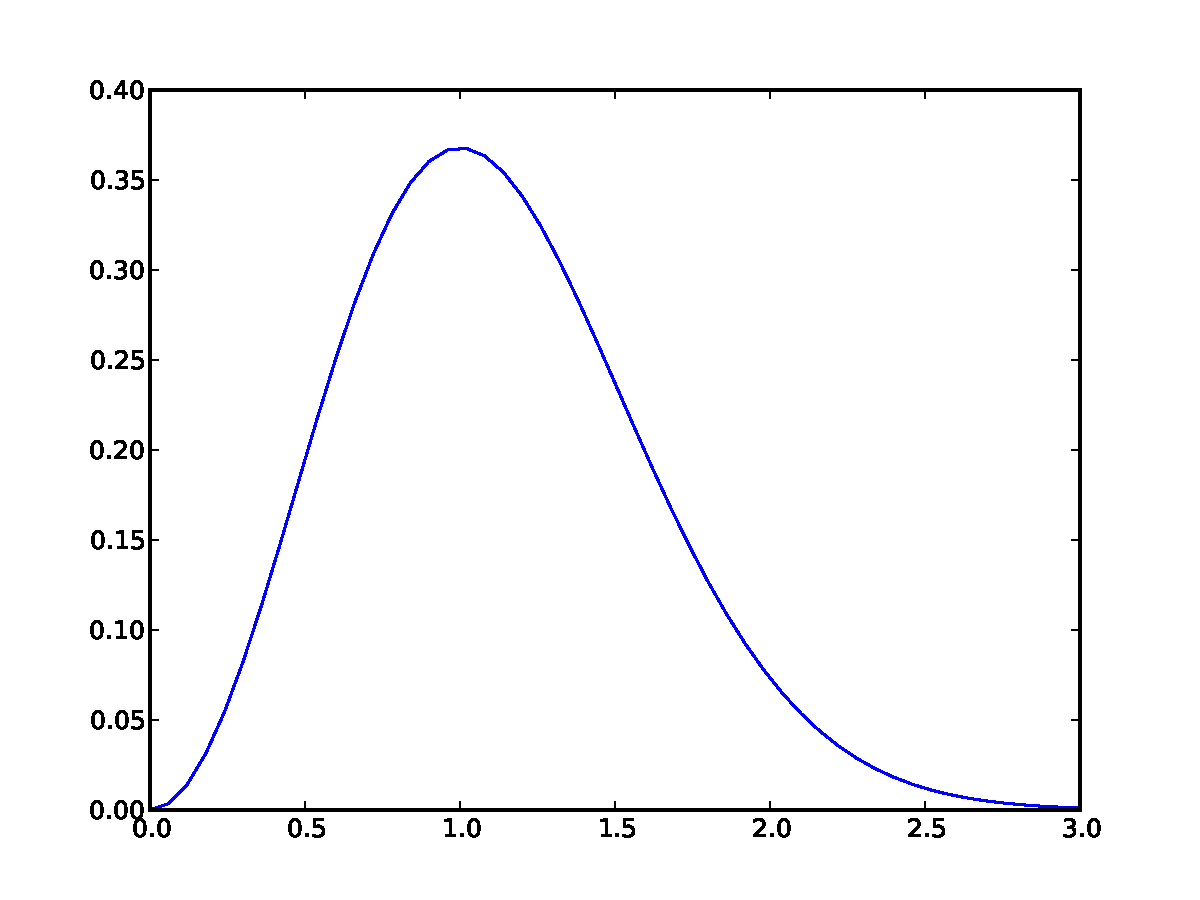
\includegraphics[width=0.5\linewidth]{../chapters/fig-plot/plot1a_pylab.pdf}}

\vspace{6mm}




The plot produced by the code above is very simple, and contains no title, axis labels, or other information.
We can easily add such information the plot using tools from \texttt{matplotlib}:
\begin{lstlisting}[language=Python,style=blue1]
import matplotlib.pyplot as plt
import numpy as np

def f(t):
    return t**2*np.exp(-t**2)

t = np.linspace(0, 3, 51)    # t coordinates
y = f(t)                  # corresponding y values

plt.plot(t, y,label="t^2*exp(-t^2)")

plt.xlabel('t')               # label on the x axis
plt.ylabel('y')               # label on the y axix
plt.legend()                  # mark the curve
plt.axis([0, 3, -0.05, 0.6])  # [tmin, tmax, ymin, ymax]
plt.title('My First Matplotlib Demo')

plt.savefig('fig.pdf')   # make PDF image for reports
plt.savefig('fig.png')   # make PNG image for web pages
plt.show()
\end{lstlisting}
Most of the lines in this code should be self-explanatory, but some are worth commenting on. The call to \texttt{legend} will
create a legend for the plot, using the information provided in the \texttt{label} argument passed to \texttt{plt.plot}. This is
very useful when plotting multiple curves in a single plot. The \texttt{axis} function will set the length of the
horisontal and vertical axes. These are otherwise set automatically to default, which usually works fine, but in
some cases the plot looks better if we set the axes manually. Later in this chapter
we will create animations of curves, and then it will be essential to set the axes to fixed lengths. Finally,
the two calls to \texttt{savefig} will save our plot in two different formats, automatically determined by the file name.



\vspace{6mm}

% inline figure
\centerline{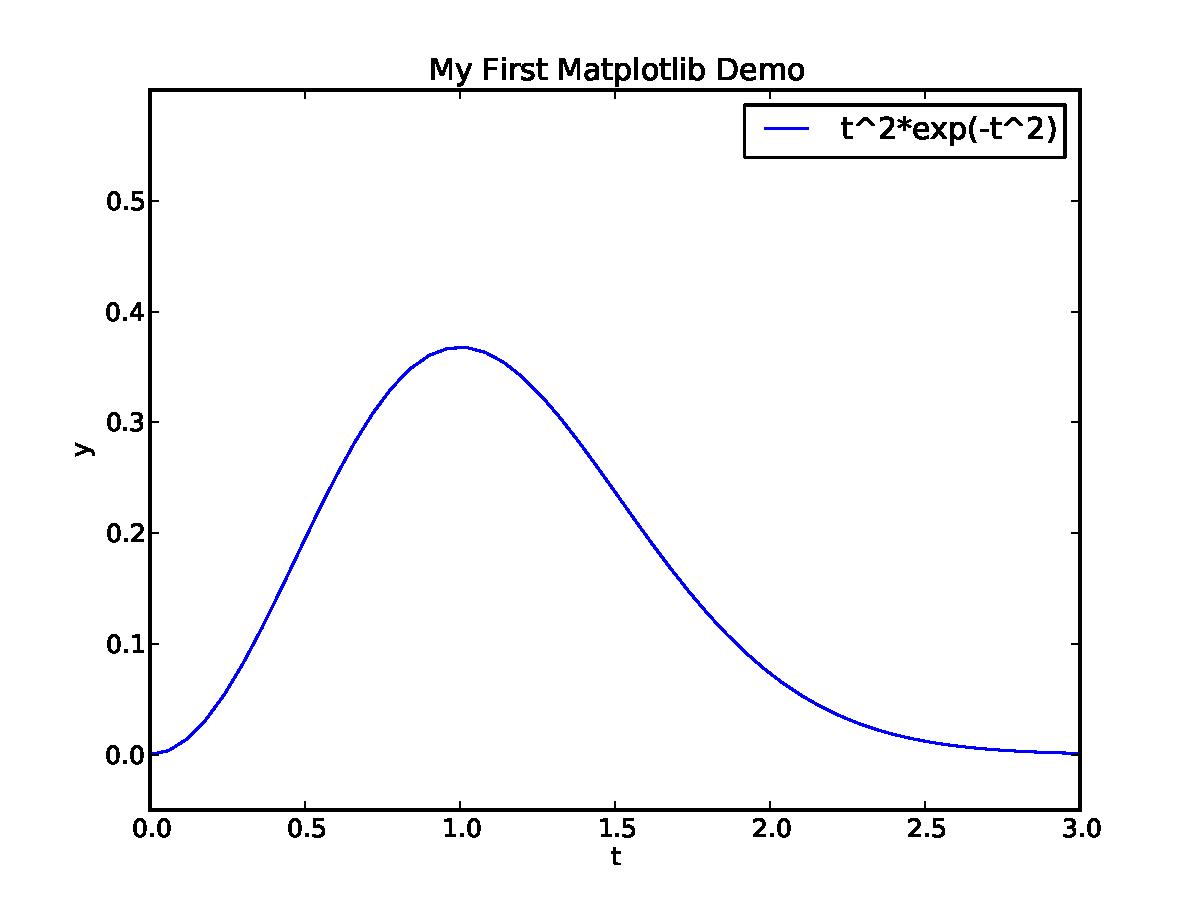
\includegraphics[width=0.9\linewidth]{../chapters/fig-plot/plot1c_pylab.pdf}}

\vspace{6mm}



As noted above, we can plot multiple curves in a single plot. In that case Matplotlib will choose the color of
each curve automatically, and this usually works well, but we can control the look of each curve if
we want to. Say we want to plot the functions $t^2e^{-t^2}$ and $t^4e^{-t^2}$ in the same plot:
\begin{lstlisting}[language=Python,style=blue1]
import matplotlib.pyplot as plt
import numpy as np

def f1(t):
    return t**2*np.exp(-t**2)

def f2(t):
    return t**2*f1(t)

t = np.linspace(0, 3, 51)
y1 = f1(t)
y2 = f2(t)

plt.plot(t, y1,  'r-', label = 't^2*exp(-t^2)') # red (r) line (-)
plt.plot(t, y2, 'bo', label = 't^4*exp(-t^2)')  # blue (b) circles (o)

plt.xlabel('t')
plt.ylabel('y')
plt.legend()
plt.title('Plotting two curves in the same plot')
plt.savefig('tmp2.png')
plt.show()
\end{lstlisting}
From this example we can see that the options for changing the color and plotting style of curves are
fairly intuitive, and can easily be explored by trial and error. For a full overview of
all the options we refer to the Matplotlib documentation.

Although the code example above was not too complex, we had to write an excess of 20 lines just to plot two simple
functions on the screen. This level of programming is needed if we want to produce professional-looking plots,
for instance for use in a presentation, a Master's thesis or a scientific report. However, if we just want a
quick plot on the screen it can be done much simpler. The following code lines will plot the same two curves as in the
example above, using just three lines:
\begin{lstlisting}[language=Python,style=blue1]
t = np.linspace(0, 3, 51)
plt.plot(t, t**2*exp(-t**2), t, t**4*exp(-t**2))
plt.show()
\end{lstlisting}
As always, the effort we put in depends on what the resulting plot will be used for, and in particular on
whether we are just exploring some data on our own or plan on presenting it to others.


\paragraph{Example: Plot a function specified on the command line.}
Say we want to write a small program \texttt{plotf.py} that allows a user to speficy a mathematical function $f(x)$ as
a command line argument, and then plots the curve $y=f(x)$. We may assume that the user should also specify the
boundaries of the curve, i.e., the lower and upper limit for $x$. The general use of the program in the terminal
should be
\begin{Verbatim}[frame=lines,label=\fbox{{\tiny Terminal}},framesep=2.5mm,framerule=0.7pt]
Terminal> python plotf.py expression xmin xmax
\end{Verbatim}
For instance, the command
\begin{Verbatim}[frame=lines,label=\fbox{{\tiny Terminal}},framesep=2.5mm,framerule=0.7pt]
Terminal> python plotf.py "exp(-0.2*x)*sin(2*pi*x)" 0 4*pi
\end{Verbatim}
Should plot the curve $y = e^{-0.2x}\sin (2\pi x)$, for $x\in [0,4\pi]$.
The \texttt{plotf.py} program should work for ``any'' mathematical expression.

We saw in the previous chapter how we could combine the \texttt{sys.argv} list of arguments with \texttt{exec} to build a Python
function for a mathematical expression. The task at hand can be solved by building on this approach,
and simply adding some statements for plotting the function at the end. However, we can make an even simpler
version, where we use \texttt{eval} to evaluate the expression directly, without even creating a Python function. The
complete code may look like this:
\begin{lstlisting}[language=Python,style=blue1]
from numpy import *
import matplotlib.pyplot as plt
import sys

formula = sys.argv[1]
xmin = eval(sys.argv[2])
xmax = eval(sys.argv[3])

x = linspace(xmin, xmax, 101)
y = eval(formula)
plt.plot(x, y)

plt.show()
\end{lstlisting}
This small program will plot any formula provided as a command-line argument. Note that in this case we have a
good reason to import NumPy with \texttt{from numpy import *}. We want the user to be able type a formula using
standard mathematical terminology, such as \texttt{sin(x) + x**2} (rather than \texttt{np.sin(x) + x**2}). For this to
work we need to import all mathematical functions from NumPy with no prefix.

\paragraph{Plotting discontinuous and piecewisely defined functions.}
Discontinuous functions, and functions defined in a piecewise manner, are common in science and engineering.
We saw in Chapter 3 how these could be implemented in Python using if-tests, but as we briefly
commented above this implementation gives rise to some challenges when using arrays and NumPy. To consider
a concrete example, say we want to plot the Heaviside function, defined by
\[ H(x) = \left\lbrace\begin{array}{ll}
0, & x<0\\ 
1, & x\geq 0
\end{array}\right.
\]
Following the ideas from Chapter 3, a Python implementation of this function may look like this
\begin{lstlisting}[language=Python,style=blue1]
def H(x):
    if x < 0:
        return 0
    else:
	return 1
\end{lstlisting}



\vspace{6mm}

% inline figure
\centerline{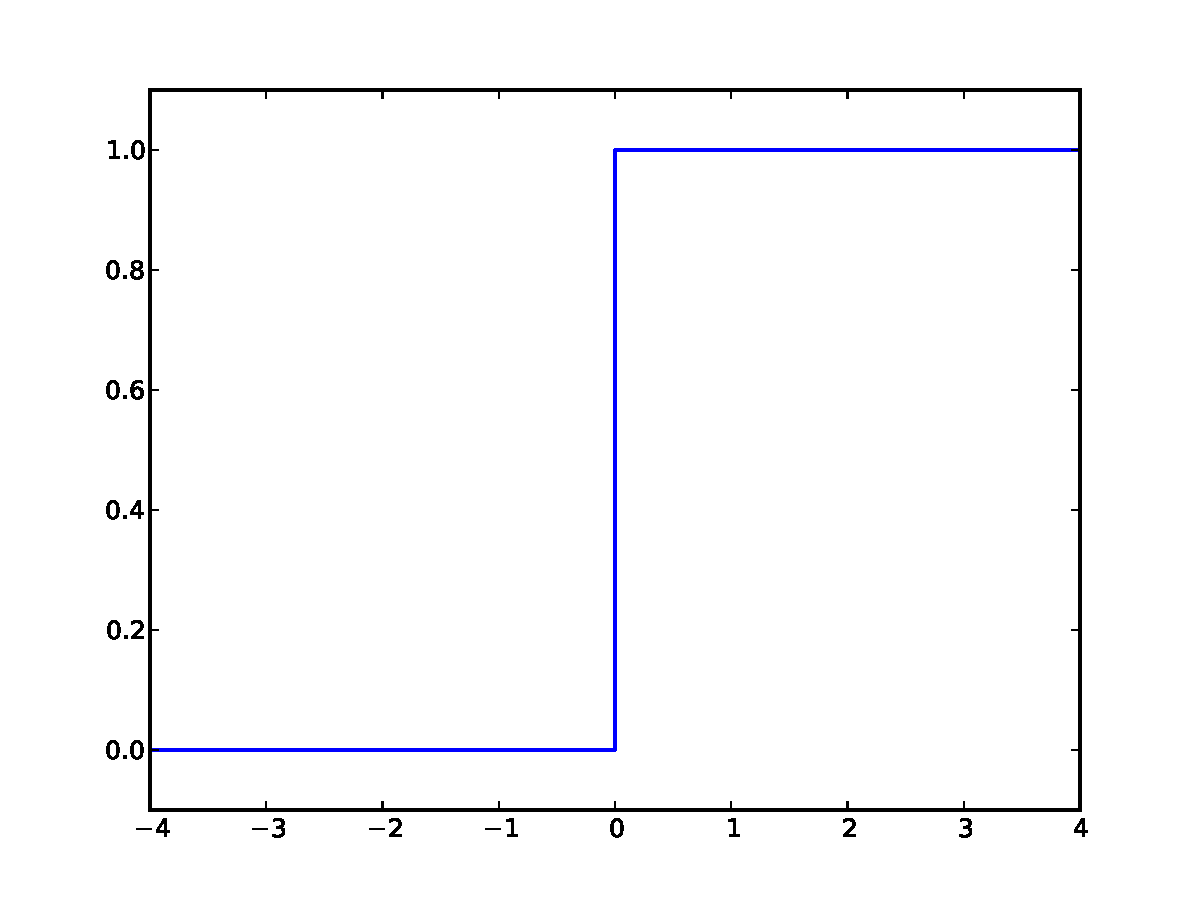
\includegraphics[width=0.5\linewidth]{../chapters/fig-plot/Heaviside3.pdf}}

\vspace{6mm}



Now we want to plot the function using the simple approach introduced above. It is natural to simply create an
array of values \texttt{x}, and pass this array to the function \texttt{H(x)} to compute the corresponding $y$-values:
\begin{lstlisting}[language=Python,style=blue1]
x = linspace(-10, 10, 5)  # few points (simple curve)
y = H(x)
plot(x, y)
\end{lstlisting}
However, if we try to run this code we get an error message, a \texttt{ValueError} error inside the function
\texttt{H(x)}, coming from the \texttt{if x < 0} line. We can illustrate what goes wrong in an interactive Python session:
\begin{lstlisting}[language=Python,style=blue1]
>>> x = linspace(-10,10,5)
>>> x
array([-10.,  -5.,   0.,   5.,  10.])
>>> b = x < 0
>>> b
array([ True,  True, False, False, False], dtype=bool)
>>> bool(b)  # evaluate b in a boolean context
...
ValueError: The truth value of an array with more than
one element is ambiguous. Use a.any() or a.all()
\end{lstlisting}
We see here that the result of the statement \texttt{b = x < 0} is an array of boolean values, whereas if \texttt{b} was a
single number the result would be a single boolean (True/False). Therefore, the statement \texttt{bool(b)}, or
tests like \texttt{if b} or \texttt{if x < 0} do not make sense, since it is impossible to say whether an array of multiple
True/False values is true or false.

There are several ways to fix this problem. One is to avoid the vectorization altogether, and go back to
the traditional for-loop for computing the values:
\begin{lstlisting}[language=Python,style=blue1]
import numpy as np
import matplotlib.pyplot as plt
n = 5
x = np.linspace(-5, 5, n+1)
y = np.zeros(n+1)

for i in range(len(x)):
    y[i] = H(x[i])

plt.plot(x,y)
plt.show()
\end{lstlisting}
A variation of the same approach is to alter the \texttt{H(x)} function itself, and put the for-loop inside it:
\begin{lstlisting}[language=Python,style=blue1]
def H_loop(x):
    r = np.zeros(len(x))  # or r = x.copy()
    for i in range(len(x)):
        r[i] = H(x[i])
    return r

n = 5
x = np.linspace(-5, 5, n+1)
y = H_loop(x)
\end{lstlisting}
We see that this latter approach ensures that we can call the function with an array argument \texttt{x}, but the
downside to both version is that we need to write quite a lot of new code, and using  a
for-loop is much slower than using vectorized array computing.

An alternative approach is to use a builtin NumPy function named \texttt{vectorize}\footnote{A fairly common misconception is to think that to vectorize a computation, or to make a vectorized version of a function, always involves using the function \texttt{numpy.vectorize}. This is not the case. In most cases we only need to make sure that we use array-ready functions such as \texttt{numpy.sin, numpy.exp}, etc. instead of the scalar version from \texttt{math}, and code all calculations so that they work on an entire array instead of stepping through the elements with a for-loop. The \texttt{vectorize}-function is usually only needed for functions containing if-tests.}, which offers automatic
vectorization of functions with if-tests. The line
\begin{lstlisting}[language=Python,style=blue1]
Hv = np.vectorize(H)
\end{lstlisting}
creates a vectorized version \texttt{Hv(x)} of the function \texttt{H(x)}, which will work  with an array argument.
This approach is obviously better, in the sense that the conversion is automatic so we need to write very little
new code, but it is actually about as slow as the two approaches based on for-loops.



A third approach is to write a new function, where the if-test is coded differently:
\begin{lstlisting}[language=Python,style=blue1]
def Hv(x):
    return np.where(x < 0, 0.0, 1.0)
\end{lstlisting}
For this particular case the NumPy function \texttt{where} will evaluate the expression \texttt{x<0}
for all elements in the array \texttt{x}, and return an array of the same length as \texttt{x}, with values 0.0
for all elements where \texttt{x<0}, and 1.0 for the rest. More generally, a function
with an if-test can be converted to an array-ready vectorized version in the following way:
\begin{lstlisting}[language=Python,style=blue1]
def f(x):
    if condition:
        x = <expression1>
    else:
        x = <expression2>
    return x

def f_vectorized(x):
    x1 = <expression1>
    x2 = <expression2>
    r = np.where(condition, x1, x2)
    return r
\end{lstlisting}
This conversion is of course not as automatic as using \texttt{vectorize}, and requires writing some more code,
but it is much more computationally efficient than the other versions. Efficiency is sometimes important when
working with large arrays.


\section{How to make a movie/animation of a plot.}
It is often useful to make animations or movies of plots, for instance if the plot represents some physical
phenomenon that actually changes with time, or if we want to visualize the effect of changing
parameters. Matplotlib has multiple tools for creating such plots, and we will explore some of them here.
To start with a specific case, consider the well-known Gaussian bell function:
\[ f(x; m, s) = {1\over\sqrt{2\pi}}{1\over s}\exp{\left[-{1\over2}\left({x-m\over s}\right)^2\right]} \]
The parameter $m$ is the location of the peak of the function, while $s$ is a measure of the width of
"bell". To illustrate the effect of these parameters, we want to make a movie (animation) of how
$f(x;m,s)$ changes shape as $s$ goes from 2 to 0.2.


% !bslidecell 01


\vspace{6mm}

% inline figure
\centerline{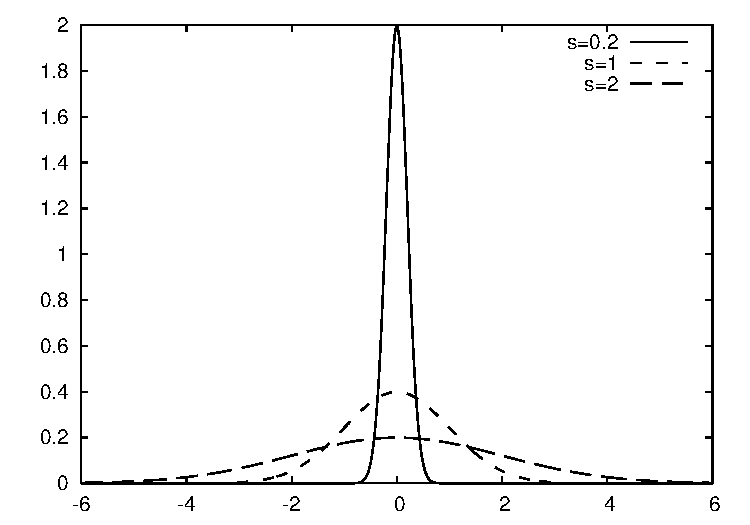
\includegraphics[width=0.8\linewidth]{../chapters/fig-plot/plot4_thick.pdf}}

\vspace{6mm}


% !eslidecell


\paragraph{Movies are made from a large set of individual plots.}
Movies of plots are created with the classical approach of cartoon movies (or really any movies), by creating a
set of images and viewing them in rapid sequence. For our specific example, the typical approach is to write a
for-loop to step through the $s$-values and either show the resulting plots directly or store them in
individual files for later processing. Regardless of which approach we use, it is imporant to always fix the
axes when making animations of plots. Otherwise, the $y$ axis always adapts to the peak of the function and
the visual impression gets completely wrong

We will look at three different ways to create a movie of the kind outlined above:
\begin{enumerate}
 \item Let the animation run \emph{live}, without saving any files. With this appraoch the plots are simply drawn on the
    screen as they are created, i.e.~one plot is shown for each pass of the for-loop. The approach is simple, but
    has the drawback that we cannot pause the movie or change the speed.

 \item Loop over all data values, plot and save the plot to file for each value, then combine all the image
    files to a movie.
    This appraoch enables us to actually create a movie file, which can be played using standard movie player
    software. The drawback of this approach is that it requires separately installed software
    (for instance \emph{ImageMagick}) to make create movie and see the animation.

 \item Use a \texttt{FuncAnimation} object from Matplotlib. This approach uses a more advanced feature of Matplotlib,
    and can be seen as a combination of the two approaches above. The animation is played \emph{live}, but can also
    be stored in an actual movie file. The downside is that the creation of the movie file still relies on
    externally installed software that needs to be integrated with Matplotlib.
\end{enumerate}

\noindent
\paragraph{Alternative one; running the movie "live" as the plots are created.}
This approach is the simplest of the three, and requires very few tools that we have not already seen. We simply
use a for-loop to loop over the $s$-values, and compute new $y$-values and update the plot for each iteration
of the loop. However, there are a couple of technical details that we need to be aware of. In particular,
the intuitive approach of simply including calls to \texttt{plot(x,y)} followed by \texttt{show()} inside the for-loop
does not work. Calling \texttt{show()} will simply make the program stop after the first plot is made, and it will not
run further until we close the plotting window. Also, recall that multiple calls to \texttt{plot} was used above
to plot multiple curves in a single window, which is not what we want here. Instead, we need to create
an object that represents the plot, and then update the $y$-values of this object for each pass through the loop.
The complete code may look like this:
\begin{lstlisting}[language=Python,style=blue1]
import matplotlib.pyplot as plt
import numpy as np

def f(x, m, s):
    return (1.0/(np.sqrt(2*np.pi)*s))*np.exp(-0.5*((x-m)/s)**2)

m = 0;  s_start = 2;  s_stop = 0.2
s_values = np.linspace(s_start, s_stop, 30)

x = np.linspace(m -3*s_start, m + 3*s_start, 1000)
# f is max for x=m (smaller s gives larger max value)
max_f = f(m, m, s_stop)

y = f(x,m,s_stop)
lines = plt.plot(x,y)  #Returns a list of line objects!

plt.axis([x[0], x[-1], -0.1, max_f])
plt.xlabel('x')
plt.ylabel('f')

for s in s_values:
    y = f(x, m, s)
    lines[0].set_ydata(y) #update plot data and redraw
    plt.draw()
    plt.pause(0.1)
\end{lstlisting}
Most of the lines in this code should be familiar, but there are a few items that are worth taking
note of. First, we use the same \texttt{plot} function as earlier, but in a slightly different manner. In general,
this function
does two things; it creates a plot that is ready to display on the screen by a subsequent call to \texttt{show()},
and it returns a special Matplotlib object which represents the plot (a \texttt{Line2D} object). In the
examples above we did not need this object, so we did not care about it, but this time we store it
in the variable \texttt{lines}.
Note also that the \texttt{plot}-function always returns a list of such objects, representing all the curves
of the plot. In this case we plot
only one curve, and the list has length one.
To update the plot inside the for-loop, we call the \Verb!set_ydata! method of this object, i.e.
\Verb!lines[0].set_ydata(y)!, every time we have computed a new \texttt{y}-array. After updating the data, we call
the function \texttt{draw()} to draw the curve on the screen. The final line inside the for-loop
simply makes the program stop and wait for 0.1 seconds. If we remove this call the movie runs too fast to
be visible at all, and we can obviously adjust the speed by changing the argument to the function.
As a final comment on this code, remember the important message from above that we always need to fix the
axes when creating movies. Otherwise Matplotlib will adjust the axes automatically for each plot,
and the resulting movie will not really look like a movie at all. Here, we compute the maximum value that the
function will obtain in the line \Verb!max_f = f(m, m, s_stop)! (based either on prior knowledge about the
Gaussian function or by inspecting the mathematical expression). This value is then used to set the axes
for all the plots that make up the movie.

\paragraph{Alternative two; save image files for later processing.}
This approach is nearly identical to the one above, but instead of showing the plots on the screen
we save them to file using the \texttt{savefig} function from Matplotlib. To avoid having each new plot over-write
the previous file, we include a counter variable and
a formatted string to create a unique file name for each iteration of the for-loop. The complete code is nearly
identical to the one above:
\begin{lstlisting}[language=Python,style=blue1]
import matplotlib.pyplot as plt
import numpy as np

def f(x, m, s):
    return (1.0/(np.sqrt(2*np.pi)*s))*np.exp(-0.5*((x-m)/s)**2)

m = 0;  s_start = 2;  s_stop = 0.2
s_values = np.linspace(s_start, s_stop, 30)

x = np.linspace(m -3*s_start, m + 3*s_start, 1000)
# f is max for x=m (smaller s gives larger max value)
max_f = f(m, m, s_stop)

y = f(x,m,s_stop)
lines = plt.plot(x,y)

plt.axis([x[0], x[-1], -0.1, max_f])
plt.xlabel('x')
plt.ylabel('f')

frame_counter = 0
for s in s_values:
    y = f(x, m, s)
    lines[0].set_ydata(y) #update plot data and redraw
    plt.draw()
    plt.savefig(f'tmp_{frame_counter:04d}.png') #unique filename
    frame_counter += 1
\end{lstlisting}
Running this program should create a number of image files, all located in the directory that we run the
program from. Converting these images into a movie requires some external software, for instance
\texttt{convert} from the ImageMagick software suite to make animated gifs, or \texttt{ffmpeg} or \texttt{avconv}
to make MP4, Flash, or other movie formats. For instance, if we want to create an animated gif of the
image files produced above, the following command will do the trick:
\begin{Verbatim}[frame=lines,label=\fbox{{\tiny Terminal}},framesep=2.5mm,framerule=0.7pt]
Terminal> convert -delay 20 tmp_*.png movie.gif
\end{Verbatim}
The resulting gif can be played using \texttt{animate} from ImageMagick or in a browser. Note that for
this approach to work, one needs to be careful about the file names. The argument \Verb!tmp_*.png! passed
to the convert function will simply replace \texttt{*} with any text, thereby sending all files with this pattern
to \texttt{convert}. The files are sent in lexicographic (i.e.~alphabetical) order, which is why we use the format
specifier \texttt{04d} in the f-string above. It would be tempting so simply write \Verb!{frame_counter}! inside the
f-string to create the unique file name, and not worry about the format specifier. This approach would create
unique filenames such as \Verb!tmp_0.png!, \Verb!tmp_1.png!, and so on. However, we would
run into problems when creating the movie with \texttt{convert}, since for instance \Verb!tmp_10.png! comes before \Verb!tmp_9.png!
in the alphabetic ordering.

\paragraph{Alternative three; use builtin Matplotlib tools.}
The third approach is the most advanced and flexible, and relies on
builtin Matplotlib tools instead of an explicit for-loop that we used above. Without the explicit for-loop
the actual steps of creating the animation are more hidden, and the approach is therefore somewhat less
intuitive. The essential steps are the following:
\begin{enumerate}
\item Make a function to update the plot. In our case this function should compute the new \texttt{y} array and call
   \Verb!set_ydata! as above to update the plot.

\item Make a list or array of the argument that changes (here $s$)

\item Pass the function and the list as arguments to create a \texttt{FuncAnimation} object
\end{enumerate}

\noindent
After creating this object, we can use various builtin methods to save the movie to a file, show it
on the screen, etc. The complete code looks as follows

\begin{lstlisting}[language=Python,style=blue1]
import numpy as np
import matplotlib.pyplot as plt
from matplotlib.animation import FuncAnimation

def f(x, m, s):
    return (1.0/(np.sqrt(2*np.pi)*s))*np.exp(-0.5*((x-m)/s)**2)

m = 0; s_start = 2; s_stop = 0.2
s_values = np.linspace(s_start,s_stop,30)

x = np.linspace(-3*s_start,3*s_start, 1000)

max_f = f(m,m,s_stop)

plt.axis([x[0],x[-1],0,max_f])
plt.xlabel('x')
plt.ylabel('y')

y = f(x,m,s_start)
lines = plt.plot(x,y) #initial plot to create the lines object

def next_frame(frame):
    y = f(x, m, frame)
    lines[0].set_ydata(y)
    return lines

ani = FuncAnimation(plt.gcf(), next_frame, frames=s_values, interval=100)
ani.save('movie.mp4',fps=20)
plt.show()
\end{lstlisting}
Most of the lines are identical to the examples above, but there are some key differences. We define a function
\Verb!next_frame! which contains all the code that updates the plot for each frame. The argument to this function
should be whatever argument that is changed for each frame (in our case $s$). After defining this function,
it is used to create a \texttt{FuncAnimation} object in the next line:
\begin{lstlisting}[language=Python,style=blue1]
ani = FuncAnimation(plt.gcf(), next_frame, frames=s_values, interval=100)
\end{lstlisting}
This function call will return an object of type \texttt{FuncAnimation} \footnote{Technically, what happens here is that we call the \emph{constructor} of the class \texttt{FuncAnimation} to create an object of this class. We will cover classes and constructors in detail in Chapter 7, but for now it is sufficient to view this as a regular function call that returns an object of type \texttt{FuncAnimation}.}.
The first argument is simply the current figure object we are working with
(\texttt{gcf} being short for \emph{get current figure}), the next is the function
we just defined to update the frames, the third is the array of \texttt{s}-values used
to create the plots, and the last argument is the interval between frames in milliseconds.
Numerous other optional arguments to the function can be used to tune the looks of the animation. We refer to the
Matplotlib documentation for the details on this.
After the object is created, we call the \texttt{save} method of the \texttt{FuncAnimation} class to create a movie file,\footnote{This call relies on some external software to be installed and integrated with Matplotlib, so it may not work on all platforms.}
or the usual \texttt{show()} to play it directly on the screen.






\subsection{More useful array operations}
At the start of this chapter we introduced the most essential operations needed for using arrays in computations and
for plotting, but NumPy arrays can do much more. Here we introduce a few additional operations that are convenient
to know about when working with arrays. First, we often need to make an array with the same size as another array. This can
be done in several ways, for instance using the \texttt{zeros} function introduced above:
\begin{lstlisting}[language=Python,style=blue1]
import numpy as np
x = np.linspace(0,10,101)
a = zeros(x.shape, x.dtype)
\end{lstlisting}
or by copying the \texttt{x} array:
\begin{lstlisting}[language=Python,style=blue1]
a = x.copy()
\end{lstlisting}
or using the convenient funtion \Verb!zeros_liks!:
\begin{lstlisting}[language=Python,style=blue1]
a = np.zeros_like(x)  # zeros and same size as x
\end{lstlisting}
If we write a function that takes either a list or an array as argument, but inside the function it needs to be an array,
we can ensure it is converted using the function \texttt{asarray}:
\begin{lstlisting}[language=Python,style=blue1]
a = asarray(a)
\end{lstlisting}
This statement will convert \texttt{a} to an array if needed (e.g., if \texttt{a} is a list or a single number), but do nothing if
\texttt{a} is already an array.

The \emph{list slicing} that we briefly introduced in Chapter 2 also works with arrays. Remember the syntax
\texttt{a[f:t:i]}, where the slice \texttt{f:t:i} implies a set of indices (from, to, increment). We can also use any list or
array of integers to index into another array:
\begin{lstlisting}[language=Python,style=blue1]
>>> a = linspace(1, 8, 8)
>>> a
array([ 1.,  2.,  3.,  4.,  5.,  6.,  7.,  8.])
>>> a[[1,6,7]] = 10
>>> a
array([  1.,  10.,   3.,   4.,   5.,   6.,  10.,  10.])
>>> a[range(2,8,3)] = -2   # same as a[2:8:3] = -2
>>> a
array([  1.,  10.,  -2.,   4.,   5.,  -2.,  10.,  10.])
\end{lstlisting}
Finally, we can use an array of boolean expressions to pick out elements of an array, as demonstrated in this
example:
\begin{lstlisting}[language=Python,style=blue1]
>>> a < 0
[False, False, True, False, False, True, False, False]
>>> a[a < 0]           # pick out all negative elements
array([-2., -2.])

>>> a[a < 0] = a.max() # if a[i]<10, set a[i]=10
>>> a
array([  1.,  10.,  10.,   4.,   5.,  10.,  10.,  10.])
\end{lstlisting}
These indexing methods can often be quite useful, since for efficiency reasons we often want to avoid for-loops to loop
over arrays elements. Many operations that are naturally implemented as for-loops can be replaced by some creative array
slicing and indexing, and the efficiency improvements may be substantial.

\subsection{Two-dimensional arrays}
Just as lists, arrays can have more than one index. Two-dimensional arrays are particularly relevant, since these
are natural representaions of for instance a table of numbers. For instance, to represent a set of numbers like
\[
\left\lbrack\begin{array}{cccc}
0 & 12 & -1 & 5\\ 
-1 & -1 & -1 & 0\\ 
11 & 5 & 5 & -2
\end{array}\right\rbrack
\]
(called a \emph{matrix} by mathematicians) it is natural to use a two-dimensional array $A_{i,j}$ with one index for the
rows and one for the columns:
\[
A =
\left\lbrack\begin{array}{ccc}
A_{0,0} & \cdots &  A_{0,n-1}\\ 
\vdots & \ddots &  \vdots\\ 
A_{m-1,0} & \cdots & A_{m-1,n-1}
\end{array}\right\rbrack
\]

In Python code, two-dimensional arrays are not much different from the one-dimensional version, except for an extra index.
Making, filling, and modifying a two-dimensional array is done in much the same way, as illustrated by this example:
\begin{lstlisting}[language=Python,style=blue1]
A = zeros((3,4))   # 3x4 table of numbers
A[0,0] = -1
A[1,0] =  1
A[2,0] = 10
A[0,1] = -5
...
A[2,3] = -100

# can also write (as for nested lists)
A[2][3] = -100
\end{lstlisting}
We can also create a nested list, as we did in Chapter 2, and convert it to an array:
\begin{lstlisting}[language=Python,style=blue1]
>>> Cdegrees = [-30 + i*10 for i in range(3)]
>>> Fdegrees = [9./5*C + 32 for C in Cdegrees]
>>> table = [[C, F] for C, F in zip(Cdegrees, Fdegrees)]
>>> print table
[[-30, -22.0], [-20, -4.0], [-10, 14.0]]
>>> table2 = array(table)
>>> print table2
[[-30. -22.]
 [-20.  -4.]
 [-10.  14.]]
\end{lstlisting}

\paragraph{Summary of useful array functionality.}


{\small   % for Springer style: small table font and more vspace

\vspace{4mm}

\begin{tabular}{ll}
\hline\noalign{\smallskip}
\multicolumn{1}{c}{ Construction } & \multicolumn{1}{c}{ Meaning } \\
\noalign{\smallskip}\svhline\noalign{\smallskip}
\texttt{array(ld)}               & copy list data \texttt{ld} to a \texttt{numpy} array                    \\
\texttt{asarray(d)}              & make array of data \texttt{d} (no data copy if already array)         \\
\texttt{zeros(n)}                & make a \texttt{float} vector/array of length \texttt{n}, with zeros     \\
\texttt{zeros(n, int)}           & make an \texttt{int} vector/array of length \texttt{n} with zeros       \\
\texttt{zeros((m,n))}            & make a two-dimensional \texttt{float} array with shape (\texttt{m},`n`) \\
\Verb!zeros_like(x)!           & make array of same shape and element type as \texttt{x}               \\
\texttt{linspace(a,b,m)}         & uniform sequence of \texttt{m} numbers in $[a,b]$                     \\
\texttt{a.shape}                 & tuple containing \texttt{a}'s shape                                   \\
\texttt{a.size}                  & total no of elements in \texttt{a}                                    \\
\texttt{len(a)}                  & length of a one-dim. array \texttt{a} (same as \texttt{a.shape[0]})     \\
\texttt{a.dtype}                 & the type of elements in \texttt{a}                                    \\
\texttt{a.reshape(3,2)}          & return \texttt{a} reshaped as $3\times 2$ array                       \\
\texttt{a[i]}                    & vector indexing                                                     \\
\texttt{a[i,j]}                  & two-dim. array indexing                                             \\
\texttt{a[1:k]}                  & slice: reference data with indices \texttt{1},\ldots,`k-1`            \\
\texttt{a[1:8:3]}                & slice: reference data with indices \texttt{1}, \texttt{4},\ldots,`7`    \\
\texttt{b = a.copy()}            & copy an array                                                       \\
\texttt{sin(a), exp(a), ...}     & \texttt{numpy} functions applicable to arrays                         \\
\texttt{c = concatenate((a, b))} & \texttt{c} contains \texttt{a} with \texttt{b} appended                   \\
\texttt{c = where(cond, a1, a2)} & \texttt{c[i] = a1[i]} if \texttt{cond[i]}, else \texttt{c[i] = a2[i]}     \\
\texttt{isinstance(a, ndarray)}  & is \texttt{True} if \texttt{a} is an array                              \\
\noalign{\smallskip}\hline\noalign{\smallskip}
\end{tabular}

\vspace{4mm}

}


\noindent
% !split
% ========= Difference equations =========
% \label{ch:diff_eq}
% # #include "../chapters/diffeq.do.txt"

% !split
\chapter{Dictionaries and strings}
\label{ch:dictstring}
% TITLE: Ch.6: Dictionaries and strings
% AUTHOR: Joakim Sundnes at Simula Research Laboratory {\&} University of Oslo, Dept.~of Informatics
% DATE: Feb 21, 2020

In this chapter we will mainly focus on two data types; dictionaries and strings. Dictionaries may
be seen as a generalization of the list datatype, where the indices are not required to be integers.
We have already used strings in all previous chapters, but we will revisit them here to introduce a
number of new and useful functions. Both dictionaries and strings are particularly useful for
reading and processing text files, and many of our examples will be related to this application.

\section{Implementing mappings in Python}
In mathematics, a mapping is a relationship between objects or structures, which often takes the
form of a function. A mapping $f$ is a rule that assigns a unique value $f(x)$ to a given input $x$.
Mappings are also widely used in computer science, and can be implemented in many different ways.
For instance, a Python list may be viewed as a mapping between integers (list indices) and the objects
contained in the list. More general mappings can be implemented using functions and if-tests, for instance
the mapping
\begin{lstlisting}[language=Python,style=blue1]
'Norway' --> 'Oslo'
'Sweden' --> 'Stockholm'
'France' --> 'Paris'
\end{lstlisting}
could be implemented in Python as
\begin{lstlisting}[language=Python,style=blue1]
def f(x):
    if x == 'Norway':
       return 'Oslo'
    elif x == 'Sweden':
       return 'Stockholm'
    elif x == 'France':
       return 'Paris'
\end{lstlisting}
Such an implementation is obviously not very convenient if we have a large number of input- and output-values.
An alternative implementation of the mapping would be to use two lists of equal length,
where for instance item  $n$ in list
\texttt{countries} correponds to item $n$ in list \texttt{capitals}. However, since such general mappings are
useful in many context, Python provides a special datastructure for them called a \emph{dictionary}. Data
structures similar to a dictionary are used in many programming languages, but often have different names.
Commonly used names are associative array, symbol table, hashmap, or simply a map.

A dictionary may be seen as a generalization of a list, where the indices are not required to be integers,
but can be any immutable Python data type. The "indices" of a dictionary are called \emph{keys}, and in this course
we will typically use strings as dictionary keys.
The dictionary implementation of the mapping above looks like
\begin{lstlisting}[language=Python,style=blue1]
d = {'Norway':'Oslo','Sweden':'Stockholm','France':'Paris'}
\end{lstlisting}
and we can look up values in the dictionary just as we would in a list, using the dictionary \emph{key}
instead of an index:
\begin{lstlisting}[language=Python,style=blue1]
print(d['Norway'])
\end{lstlisting}
To extend the dictionary with new values, we can simply write
\begin{lstlisting}[language=Python,style=blue1]
d['Germany'] = Berlin
\end{lstlisting}
Notice this important difference between a list and a dictionary. For a list we had to use \texttt{append()} to
add new elements. A dictionary has no \texttt{append} method, and to extend it we simply introduce a new key
and corresponding value.

Dictionaries can be initialized in two different ways. One is by using the curly brackets, as in the example
above. Alternatively, we can use the built-in function \texttt{dict}, which takes a number of key-value pairs as
arguments and returns the corresponding dictionary. The two approaches may look like this:
\begin{lstlisting}[language=Python,style=blue1]
mydict = {'key1': value1, 'key2': value2, ...}

temps = {'Oslo': 13, 'London': 15.4, 'Paris': 17.5}

# or
mydict = dict(key1=value1, key2=value2, ...)

temps = dict(Oslo=13, London=15.4, Paris=17.5)
\end{lstlisting}
Notice the differences in syntax. When initializing using the curly brackets we
use colon to separate the key from its corresponding value, and the key can be any immutable Python object
(strings in the example above). When using the \texttt{dict} function, we pass the key-value pairs as \emph{keyword arguments}
to the function,
and the keywords are converted to keys of type string. However, in both cases the initialization involves defining
a set of key-value pairs to populate the dictionary. A dictionary is simply an unordered collection of such
key-value pairs.

We are used to looping over lists to access the individual elements. We can do the same with dictionaries, with the
small but important difference that looping over a dictionary means looping over the keys, not the values. If we
want to access the values we need to look them up in the dictionary using the keys. For instance, generic code
to print all the values of a dictionary would look as follows:
\begin{lstlisting}[language=Python,style=blue1]
for key in dictionary:
    value = dictionary[key]
    print(value)
\end{lstlisting}
A conrete example based on the example above may look like
\begin{lstlisting}[language=Python,style=blue1]
temps = {'Oslo': 13, 'London': 15.4, 'Paris': 17.5, 'Madrid': 26}
for city in temps:
    print(f'The {city} temperature is temps{city}')
\end{lstlisting}
Output:
\begin{lstlisting}[language=Python,style=gray]
The Paris temperature is 17.5
The Oslo temperature is 13
The London temperature is 15.4
The Madrid temperature is 26
\end{lstlisting}
As mentioned above, a dictionary is an \emph{unordered} collection of key-value pair, meaning that the
sequence of the keys in the dictionary is arbitrary. If we want to print or otherwise process
the elements in a particular order the keys first need to be sorted, for instance using the builtin
function \texttt{sorted}:
\begin{lstlisting}[language=Python,style=blue1]
for city in sorted(temps):   # alphabetic sort of keys
    value = temps[city]
    print value
\end{lstlisting}
There may be applications where sorting the keys like this is important, but usually the order of a dictionary
is insignificant. In most applications where the order of the elements is important, a list or an array is a more
convenient data type than a dictionary.

\paragraph{Dictionaries and lists share many similarities.}
Much of the functionality that we are familiar with for list also exists for dictionaries. We can, for instance,
check if a dictionary has a particular key with the expression \texttt{key in dict}, which returns True or False:
\begin{lstlisting}[language=Python,style=blue1]
>>> if 'Berlin' in temps:
...     print('Berlin:', temps['Berlin'])
... else:
...     print('No temperature data for Berlin')
...
No temperature data for Berlin
>>> 'Oslo' in temps     # standard boolean expression
True
\end{lstlisting}
Deleting an element of a dictionary is done exactly as with lists, using the operator \texttt{del}:
\begin{lstlisting}[language=Python,style=blue1]
>>> del temps['Oslo']   # remove Oslo key w/value
>>> temps
{'Paris': 17.5, 'London': 15.4, 'Madrid': 26.0}
>>> len(temps)          # no of key-value pairs in dict.
3
\end{lstlisting}
In some cases it may be useful to access the keys or values of a dictionary as separate entities, and this can be
obtained with the methods \texttt{keys} and \texttt{values}, for instance
\texttt{temps.keys()} and \texttt{temps.values()} for the case above. These methods will return \emph{iterators}, which are
list-like objects that can be looped over or converted to a list:
\begin{lstlisting}[language=Python,style=blue1]
>>> for temp in temps.values():
>>>    print(temp)
...
17.5
15.4
26.0
>>> keys_list = list(temps.keys())
\end{lstlisting}

Just as with lists, when we assign an existing dictionary to a new variable, the dictionary is not copied. Instead,
the new variable name becomes a \emph{reference} to the same dictionary, and changing it will also change the original
variable. The following code illustrates the behavior:
\begin{lstlisting}[language=Python,style=blue1]
>>> t1 = temps
>>> t1['Stockholm'] = 10.0    # change t1
>>> temps                     # temps is also changed!
{'Stockholm': 10.0, 'Paris': 17.5, 'London': 15.4,
  'Madrid': 26.0}
>>> t2 = temps.copy()         # take a copy
>>> t2['Paris'] = 16
>>> t1['Paris']               # t1 was not changed
17.5
\end{lstlisting}
Here, the call to \texttt{temps.copy()} ensures \texttt{t2} is a copy of the original dictionary, and not a reference, so changing
it does not alter the original dictionary. Recall that lists behave in the same way:
\begin{lstlisting}[language=Python,style=blue1]
>>> L = [1, 2, 3]
>>> M = L
>>> M[1] = 8
>>> L[1]
8
>>> M = L.copy() #for lists, M = L[:]  also works
>>> M[2] = 0
>>> L[2]
3
\end{lstlisting}

So far we have used texts (string objects) as keys, but the keys of a dictionary can be any \emph{immutable} (constant) object.
For instance, we can use integers, floats, and tuples as keys, but not lists since they are mutable objects:
\begin{lstlisting}[language=Python,style=blue1]
>>> d = {1: 34, 2: 67, 3: 0}   # key is int
>>> d = {13: 'Oslo', 15.4: 'London'} # possible
>>> d = {(0,0): 4, (1,-1): 5}  # key is tuple
>>> d = {[0,0]: 4, [-1,1]: 5}  # list is mutable/changeable
...
TypeError: unhashable type: 'list'
\end{lstlisting}
Of course, the fact that these alternatives work in Python does not mean that they are recommended or very useful.
It is, for instance, hard to imagine a useful application for a dictionary with a temperature as key and a
city name as value. Strings are the most obvious and commonly used data type for dictionary keys, and will also be
the most common through this course. However, there are applications where other types of keys are useful, as we
will see in the following examples.

\paragraph{Example; representing a polynomial with a dictionary.}
The information in the polynomial
\[ p(x)=-1 + x^2 + 3x^7 \]
can be represented by a dictionary with power as key (\texttt{int}) and
coefficient as value (\texttt{float} or   \texttt{int}):
\begin{lstlisting}[language=Python,style=blue1]
p = {0: -1, 2: 1, 7: 3}
\end{lstlisting}
More generally, a polynomial written on the form
\[
p(x) = \sum_{i\in I}^N c_i x^i ,
\]
for some set of integers $I$, can represented by a dictionary with keys $i$ and values $c_i$.
To evaluate a polynomial represented by such a dictionary, we need to iterate over keys dictionary, extract the
corresponding values, and sum up the terms. The following function takes two arguments; a dictionary \texttt{poly} and a number
or array \texttt{x}, and evaluates the polynomial in \texttt{x}:
number (or array) $x$:
\begin{lstlisting}[language=Python,style=blue1]
def eval_poly_dict(poly, x):
    sum = 0.0
    for power in poly:
        sum += poly[power]*x**power
    return sum
\end{lstlisting}
We see that the function follows our standard recipe for evaluating a sum;
set a summation variable to zero and then add in all the terms using a for-loop. We can write an even
shorter version of the function using Python's builtin function \texttt{sum}:
\begin{lstlisting}[language=Python,style=blue1]
def eval_poly_dict(poly, x):
    # Python's sum can add elements of an iterator
    return sum(poly[power]*x**power for power in poly)
\end{lstlisting}

Since the keys of the polynomial dictionary are integers, we could also replace the dictionary
with a list, where the list index corresponds to the power of the respective term.
The polynomial above, i.e.~$-1 + x^2 + 3x^7$ can be represented as the list
\begin{lstlisting}[language=Python,style=blue1]
p = [-1, 0, 1, 0, 0, 0, 0, 3]
\end{lstlisting}
and the general polynomial $\sum_{i=0}^N c_ix^i$ is stored as
\texttt{[c0, c1, c2, ..., cN]}. The function to evaluate a polynomial represented by a list is
nearly identical to the function for the dictionary. The function
\begin{lstlisting}[language=Python,style=blue1]
def eval_poly_list(poly, x):
    sum = 0
    for power in range(len(poly)):
        sum += poly[power]*x**power
    return sum
\end{lstlisting}
will evaluate a polynomial $\sum_{i=0}^N c_ix^i$ for a given $x$. Although the two
representations are very similar, the list representation has the obvious disadvantage
that we need to store all the zeros. For "sparse" polynomials of high order this can be
quite inconvenient, and the dictionary representation is obviously better.
The dictionary representation can also easily handle negative powers,
for instance $\frac{1}{2} x^{-3} + 2x^4$:
\begin{lstlisting}[language=Python,style=blue1]
p = {-3: 0.5, 4: 2}
print eval_poly_dict(p, x=4)
\end{lstlisting}
This code will work just fine without any modifications of the \Verb!eval_poly_dict!
function. Lists in Python cannot have negative indices (since indexing a list with a negative number
implies counting indices from the end of the list), and it is not trivial to extend the list representation to
handle negative powers.

\paragraph{Example; read file data into a dictionary.}
Say we have a file \texttt{deg2.dat}, containing temperature data for a number of cities:
\begin{lstlisting}[language=Python,style=gray]
Oslo:          21.8
London:        18.1
Berlin:        19
Paris:         23
Rome:          26
Helsinki:      17.8
\end{lstlisting}
We now want to read this file and store the information in a dictionary, with the
city names as keys and the temperatures as values. The recipe is nearly identical to
the one we previously used for reading file data into lists; first create an empty dictionary, then
fill it with values read from the file:
\begin{lstlisting}[language=Python,style=blue1bar]
with open('deg2.dat', 'r') as infile:
    temps = {}                  # start with empty dict
    for line in infile:
        city, temp = line.split()
        city = city[:-1]        # remove last char (:)
        temps[city]  = float(temp)
\end{lstlisting}
The only real difference between this code and previous examples based on lists
is the way we add new data to the dictionary. We used the the
\texttt{append} method to populate an empty list, but dictionaries have no such method. Instead,
we add a new key-value pair with the line \texttt{temps[city] = float(temp)}. Apart from this technical
difference, the recipe for populating a dictionary is exactly the same as for lists.


\section{String manipulation}
We have already worked with strings in previous chapters, for instance the very
useful \texttt{split}-method:
\begin{lstlisting}[language=Python,style=blue1]
>>> s = 'This is a string'
>>> s.split()
['This', 'is', 'a', 'string']
\end{lstlisting}
String manipulation is essential for reading and interpreting the content of files,
and the way we process files is often quite dependent on the file structure. For
instance, we need to know on which line the relevant information starts, how data items
are separated, and how many data items there are on each line. The algorithm for reading and processing
the text needs to be tailored to the structure of the file. Although the \texttt{split} function already considered is quite
flexible, and covers most of our needs in this course, it may not
always be the best tool. Python has a number of other ways to process strings,
which may in some cases make the text processing easier and more efficient.

Text in Python is represented by string objects (of type \texttt{str}). To introduce some
of the basic operations on strings, we consider the example string:
\begin{lstlisting}[language=Python,style=blue1]
>>> s = 'Berlin: 18.4 C at 4 pm'
\end{lstlisting}
Such a string is really just a sequence of characters, and it behaves much like
other sequence data types such as lists and tuples. For instance,
we can index a string to extract individual characters;
\begin{lstlisting}[language=Python,style=blue1]
>>> s[0]
'B'
>>> s[1]
'e'
>>> s[-1]
'm'
\end{lstlisting}
Slices also work as we are used to, and can be used to extract substrings of a string:
\begin{lstlisting}[language=Python,style=blue1]
>>> s
'Berlin: 18.4 C at 4 pm'
>>> s[8:]     # from index 8 to the end of the string
'18.4 C at 4 pm'
>>> s[8:12]   # index 8, 9, 10 and 11 (not 12!)
'18.4'
>>> s[8:-1]
'18.4 C at 4 p'
>>> s[8:-8]
'18.4 C'
\end{lstlisting}
Iterating over a string also works as we would expect:
\begin{lstlisting}[language=Python,style=blue1]
>>> s = 'Berlin: 18.4 C at 4 pm'
>>> for s_ in s:
    	print(s_, end=' ')
\end{lstlisting}

Strings have a method named \texttt{find}, which searches a string for a given substring, and returns
the index of its location:
\begin{lstlisting}[language=Python,style=blue1]
>>> s.find('Berlin')  # where does 'Berlin' start?
0                     # at index 0
>>> s.find('pm')
20
>>> s.find('Oslo')    # not found
-1
\end{lstlisting}
Lists do not have \texttt{find}-method, but we have seen previously seen the list's \texttt{index} method,
which is quite similar. Strings also have a method named \texttt{index}, which does almost the same thing
as \texttt{find}. However, while \texttt{find} will return $-1$ if the substring does not exist in the string, \texttt{index}
will end with an error message. If we want to know if a substring is part of a string, and don't really
care about its location, we can also use \texttt{in}:
\begin{lstlisting}[language=Python,style=blue1]
>>> 'Berlin' in s:
True
>>> 'Oslo' in s:
False

>>> if 'C' in s:
...     print 'C found'
... else:
...     print 'no C'
...
C found
\end{lstlisting}
We may recall from Chapter 2 that this use of \texttt{in} is almost exactly the same as for lists and tuples. The
only minor difference is that for lists and tuples we can only check for the existence of an individual
element, while for strings it works for a substring of arbitrary length.

In many cases we are interested not only in finding a substring, but to find it and replace it with something else.
For this task we have a string method named \texttt{replace}. It takes two strings as arguments, and a call
like \texttt{s.replace(s1, s2)} will replace \texttt{s1} by \texttt{s2} everywhere in \texttt{s}. The following examples illustrate how
it is used;
\begin{lstlisting}[language=Python,style=blue1]
>>> s = 'Berlin: 18.4 C at 4 pm'
>>> s.replace(' ', '__')
'Berlin:__18.4__C__at__4__pm'
>>> s.replace('Berlin', 'Bonn')
'Bonn: 18.4 C at 4 pm'
>>> s.replace(s[:s.find(':')], 'Bonn')
'Bonn: 18.4 C at 4 pm'
\end{lstlisting}
In the final example we combine \texttt{find} and replace to replace all text before the \texttt{':'} with \texttt{'Bonn'}. First,
\texttt{s.find(':')} returns 6, which is the index where the \texttt{':'} is found, then the slice
\texttt{s[:6]} is \texttt{'Berlin'}, which is replaced by \texttt{'Bonn'}.

\paragraph{Splitting and joining strings.}
We have already introduced the \texttt{split} method, which is arguably the most useful method for reading
and processing text files. As we recall from Chapter 4, the call \texttt{s.split(sep)} will split the string \texttt{s}
into a list of substrings separated by \texttt{sep}. The \texttt{sep} argument is optional, and if it is omitted the string
is split with respect to whitespace. Consider these two simple examples to recall how it is used;
\begin{lstlisting}[language=Python,style=blue1]
>>> s = 'Berlin: 18.4 C at 4 pm'
>>> s.split(':')
['Berlin', ' 18.4 C at 4 pm']
>>> s.split()
['Berlin:', '18.4', 'C', 'at', '4', 'pm']
\end{lstlisting}
The \texttt{split} method has an "inverse" called \texttt{join}, which is used to put a list of strings together with a
delimiter in between:
\begin{lstlisting}[language=Python,style=blue1]
>>> strings = ['Newton', 'Secant', 'Bisection']
>>> ', '.join(strings)
'Newton, Secant, Bisection'
\end{lstlisting}
Notice that we call the \texttt{join} method belonging to the delimiter \texttt{', '}, which is a string object, and pass the list of
strings as argument. If we want to put the same list together separated by whitespace, we would simply
replace \texttt{', '.join(strings)} in the example above with \texttt{' '.join(strings)}.

Since \texttt{split} and \texttt{join} are inverse operations, using them in sequence will give back the original string,
as in the following example;
\begin{lstlisting}[language=Python,style=blue1]
>>> l1 = 'Oslo: 8.4 C at 5 pm'
>>> words = l1.split()
>>> l2 = ' '.join(words)
>>> l1 == l2
True
\end{lstlisting}
A common usecase for the join method is to split off a known number of words on a line. Say we want to read
a file on the following format, and combine the city name and the country into a single string;
\begin{lstlisting}[language=Python,style=gray]
Tromsø Norway 69.6351 18.9920 52436
Molde Norway 62.7483 7.1833 18594
Oslo Norway 59.9167 10.7500 835000
Stockholm Sweden 59.3508 18.0973 1264000
Uppsala Sweden 59.8601 17.6400 133117
\end{lstlisting}
The following code will read such a file and create a dictionary with the data
\begin{lstlisting}[language=Python,style=blue1]
cities = {}
with open('cities.txt') as infile:
    for line in infile:
        words = line.split()
	name = ', '.join(words[:2])
	data = {'lat': float(words[2]),  'long':float(words[3])}
	data['pop'] = int(words[3])
	cities[name] = data
\end{lstlisting}
Here the line \texttt{name = ', '.join(words[:2])} creates strings like \texttt{'Tromsø, Norway'}, which are then used as dictionary keys.

In most of the examples considered so far we have read and processed text files line by line, but in some cases we have a string with lots of text in multiple lines,
and we want to split it into single lines. We can do this using the \texttt{split} method with the appropriate separator. For instance, on Linux and Mac systems the line separator
is  \Verb!\n!;
\begin{lstlisting}[language=Python,style=blue1]
>>> t = '1st line\n2nd line\n3rd line'
>>> print t
1st line
2nd line
3rd line
>>> t.split('\n')
['1st line', '2nd line', '3rd line']
\end{lstlisting}
This example works fine on Mac or Linux, but the line separator on Windows is not \Verb!\n!, but \Verb!\r\n!,
and to have a platform independent solution
it is better to use the method \texttt{splitlines()}, which works with
both line separators;
\begin{lstlisting}[language=Python,style=blue1]
>>> t = '1st line\n2nd line\n3rd line'	   #Unix format
>>> t.splitlines()
['1st line', '2nd line', '3rd line']
>>> t = '1st line\r\n2nd line\r\n3rd line' # Windows
>>> t.splitlines()                         # cross platform!
['1st line', '2nd line', '3rd line']
\end{lstlisting}

\paragraph{Strings are constant - immutable - objects.}
In many of the examples above we have highlighted the similarity between strings and lists, since we are
very familiar with lists from earlier chapters. However, strings are even more similar to tuples, since they are
immutable objects. We could change elements of a list in-place by indexing into the list, but this does not
work for strings. Trying to assign a new value to a part of a string will result in an error message:
\begin{lstlisting}[language=Python,style=blue1]
>>> s[18] = 5
...
TypeError: 'str' object does not support item assignment
\end{lstlisting}
Instead, to perform such a replacement we can build a new string manually by adding pieces of the original string,
or use the \texttt{replace} method introduced above:
\begin{lstlisting}[language=Python,style=blue1]
>>> # build a new string by adding pieces of s:
>>> s2 = s[:18] + '5' + s[19:]
>>> s2
'Berlin: 18.4 C at 5 pm'
>>> s2 = s.replace(s[18],5)
>>> s2
'Berlin: 18.4 C at 5 pm'
\end{lstlisting}
Some may find it confusing that strings are immutable, but they still have a method like \texttt{replace}, which apparently
alters the string. How can we replace a substring with another if strings are immutable objects?
The answer is that \texttt{replace} does not really change the original string, but returns
a new one. This behavior is similar to for instance the call \texttt{s.split()}, which will not turn \texttt{s} into a list but
instead leave \texttt{s} unchanged and \emph{return} a list of the substrings. Similarly, a call like \texttt{s.replace(4,5)} does
not change \texttt{s} but it will return a new string that we can assign either to \texttt{s} or some other variable name,
as we did in the example above. The call \texttt{s.replace(4,5)} does nothing useful on its own, unless it is combined
into an assignment such as \texttt{s2 = s.replace(4,5)} or \texttt{s = s.replace(4,5)}.


\paragraph{Other convenient string methods in Python.}
It is often convenient to strip off leading or trailing whitespace from a string, and there are methods \texttt{strip(), lstrip()} and
\texttt{rstrip()} for doing this:
\begin{lstlisting}[language=Python,style=blue1]
>>> s = '   text with leading/trailing space   \n'
>>> s.strip()
'text with leading/trailing space'
>>> s.lstrip()   # left strip
'text with leading/trailing space   \n'
>>> s.rstrip()   # right strip
'   text with leading/trailing space'
\end{lstlisting}
We can also check whether a string is only contains numbers (digits), only space, or if a string starts or ends with a given substring;
\begin{lstlisting}[language=Python,style=blue1]
>>> '214'.isdigit()
True
>>> '  214 '.isdigit()
False
>>> '2.14'.isdigit()
False

>>> '    '.isspace()   # blanks
True
>>> '  \n'.isspace()   # newline
True
>>> '  \t '.isspace()  # TAB
True
>>> ''.isspace()       # empty string
False

>>> s.startswith('Berlin')
True
>>> s.endswith('am')
False
\end{lstlisting}
Finally, we may be interested in converting between lower case and upper case characters;
\begin{lstlisting}[language=Python,style=blue1]
>>> s.lower()
'berlin: 18.4 c at 4 pm'
>>> s.upper()
'BERLIN: 18.4 C AT 4 PM'
\end{lstlisting}
The examples shown here are just a few of the useful string operations defined in Python. Many more exist, but all the
text processing tasks in this course can be accomplished with the operations listed here. In fact, nearly all the tasks
we encounter can be solved by using a combination of \texttt{split} and \texttt{join} in addition to indexing and slicing of strings.

\paragraph{Example; read pairs of numbers (x,y) from a file.}
To summarize some string operations using an example, consider the task of reading files on the following format;
\begin{lstlisting}[language=Python,style=gray]
(1.3,0)    (-1,2)    (3,-1.5)
(0,1)      (1,0)     (1,1)
(0,-0.01)  (10.5,-1) (2.5,-2.5)
\end{lstlisting}
We want to read these coordinate pairs, converted the numbers to floats, and store them as a list of tuples. The algorithm
is similar to how we have processed files earlier:
\begin{enumerate}
\item Read line by line

\item For each line, split the line into words

\item For each word, strip off the paretheses
   and split the rest with respect to comma to extract the numbers
\end{enumerate}

\noindent
From these operations, we may observe that the \texttt{split} is a useful tool, as usual when processing text files. For stripping
parantheses off the coordinate pairs we can for instance use slicing. Translated into code, the example may look like this:
\begin{lstlisting}[language=Python,style=blue1]
lines = open('read_pairs.dat', 'r').readlines()

pairs = []   # list of (n1, n2) pairs of numbers
for line in lines:
    words = line.split()
    for word in words:
        word = word[1:-1]  # strip off parenthesis
        n1, n2 = word.split(',')
        n1 = float(n1);  n2 = float(n2)
        pair = (n1, n2)
        pairs.append(pair)
\end{lstlisting}

\section{Summary of dictionary and string functionality}
The following table lists some useful functionality of dictionaries:



{\small   % for Springer style: small table font and more vspace

\vspace{4mm}

\begin{tabular}{ll}
\hline\noalign{\smallskip}
\multicolumn{1}{c}{ Construction } & \multicolumn{1}{c}{ Meaning } \\
\noalign{\smallskip}\svhline\noalign{\smallskip}
\Verb!a = {}!                             & initialize an empty dictionary                          \\
\Verb!a = {'point': [0,0.1], 'value': 7}! & initialize a dictionary                                 \\
\texttt{a = dict(point=[2,7], value=3)}     & initialize a dictionary w/string keys                   \\
\texttt{a.update(b)}                        & add/update key-value pairs from \texttt{b} in \texttt{a}    \\
\texttt{a.update(key1=value1, key2=value2)} & add/update key-value pairs in \texttt{a}                  \\
\texttt{a['hide'] = True}                   & add new key-value pair to \texttt{a}                      \\
\texttt{a['point']}                         & get value corresponding to key \texttt{point}             \\
\texttt{for key in a:}                      & loop over keys in unknown order                         \\
\texttt{for key in sorted(a):}              & loop over keys in alphabetic order                      \\
\texttt{'value' in a}                       & \texttt{True} if string \texttt{value} is a key in \texttt{a} \\
\texttt{del a['point']}                     & delete a key-value pair from \texttt{a}                   \\
\texttt{list(a.keys())}                     & list of keys                                            \\
\texttt{list(a.values())}                   & list of values                                          \\
\texttt{len(a)}                             & number of key-value pairs in \texttt{a}                   \\
\texttt{isinstance(a, dict)}                & is \texttt{True} if \texttt{a} is a dictionary              \\
\noalign{\smallskip}\hline\noalign{\smallskip}
\end{tabular}

\vspace{4mm}

}


\noindent
The following code summarizes most of the string functionality introduced above:
\begin{lstlisting}[language=Python,style=blue1]
s = 'Berlin: 18.4 C at 4 pm'
s[8:17]          # extract substring
s.find(':')      # index where first ':' is found
s.split(':')     # split into substrings
s.split()        # split wrt whitespace
'Berlin' in s    # test if substring is in s
s.replace('18.4', '20')
s.lower()        # lower case letters only
s.upper()        # upper case letters only
s.split()[4].isdigit()
s.strip()        # remove leading/trailing blanks
', '.join(list_of_words)
\end{lstlisting}

% !split
\chapter{Classes}
\label{ch:classes}
% TITLE: Ch.7: Introduction to classes
% AUTHOR: Joakim Sundnes at Simula Research Laboratory {\&} University of Oslo, De
% DATE: Feb 21, 2020


In this chapter we will introduce classes, which is a fundamental concept in programming. Most modern
programming languages support classes or similar concepts, and we have already used classes extensively throughout this
book. Recall how we could check the type of a variable with the \texttt{type} method, and the output would be on the form
\texttt{<class 'int'>},  \texttt{<class 'float'>}, etc. This simply states that the type of an object is defined in the form of a class.
Every time we create for instance an integer variable in our program, we create an object or \emph{instance} of the \texttt{int} class.
The class defines how the objects behave and what methods they contain. We have used a number of different methods bound
to objects, such as the \texttt{append} method for list objects, \texttt{split} for strings, and many more. All such methods are
part of the definition of the class that the object belongs to. So far we have only used Python's builtin classes to create
objects, but in this chapter we will write our own classes and use them to create objects tailored to our particular needs.

\section{Basics of classes}
A class packs together data and functions, or methods, in a single unit. As we have seen in previous chapters, functions
that are bound to a class or objects are usually called methods, and we will stick to this notation in the present chapter.
Classes have some similarity with modules, which are also collections of variables and functions that naturally
belong together. However, while there is only a single instance of a module, we can create multiple instances of a
class. Different instances of the same class may contain different data, but they all behave in the same way. and have the
same methods. Think of a basic Python class like \texttt{int}; we can create many integer variables in a program, and they
obviously have different values (data), but we know that they all have the same general behavior and the same
set of operations defined for them. The same goes for more complex Python classes like lists and strings; different
objects contain different data but they all have the same methods. The classes we will create in this chapter behaves
in exactly the same way.


\paragraph{First example; a class representing a function.}
To start with a familiar example, consider the function introduced earlier that defines the height of an object as a
function of $t$:
\[ y(t; v_0)=v_0t - {1\over2}gt^2\]
We need both $v_0, t$, and $g$ to compute $y$., but
how should we implement this? It is natural to think of $g$ as constant, but both $v_0$ and $t$ may vary with every call.
However, for many applications of functions of this kind $t$ will vary much more frequently than $v_0$. Since $v_0$
can be thought of as a parameter in a model, it is quite common to call such a function many times with the same $v_0$
but different $t$-values. How should we implement this in a convenient way? The default solution would be
to have both $t$ and $v_0$ as arguments, possibly with a default value for $v_0$:
\begin{lstlisting}[language=Python,style=blue1]
def y(t, v0 = 5):
    g = 9.81
    return v0*t - 0.5*g*t**2
\end{lstlisting}
This solution obviously works, but if we want a different value of $v_0$ we need to pass the value to the function every time
it is called. And what if the function is to be passed as an argument to another function, which expects it to take a
single argument only? \footnote{This situation is fairly common in Python programs. Consider for instance the function implementing Newton's method in Appendix A. This function takes two functions as arguments, and because of how they are used inside the function both need to take a single argument (\texttt{x}). If we want to pass a parameterized function as argument to such a function, it needs to be modified.}

Another solution would to have $t$ as argument and $v_0$ as global variable:
\begin{lstlisting}[language=Python,style=blue1]
def y(t):
    g = 9.81
    return v0*t - 0.5*g*t**2
\end{lstlisting}
We now have a function which only takes a single argument, but defining \texttt{v0} as a global variable is not very convenient
if we want to evaluate \texttt{y(t)} for different values of \texttt{v0}. A third possible solution would be to set
\texttt{v0} as a local variable inside the function, and define different functions \texttt{y1(t), y2(t), y3(t)}, etc. for each value
of \texttt{v0}. This solution is obviously not very convenient if we want many values of \texttt{v0}, but we shall see that programming
with classes and objects offers exactly that; a convenient solution to create a family of similar functions.




\paragraph{Representing a function by a class.}
With a class, \texttt{y(t)} can be a function of \texttt{t} only, but still have \texttt{v0} and \texttt{g} as parameters with given values.
The class packs together a function (or method) \texttt{y(t)} and data (\texttt{v0}, \texttt{g}).
We make a class \texttt{Y} for $y(t;v_0)$ with variables \texttt{v0} and \texttt{g} and a function \texttt{value(t)} for computing $y(t;v_0)$.
All classes should also have a function named \Verb!__init__! for initializing the variables. The following code defines our function class
\begin{lstlisting}[language=Python,style=blue1]
class Y:
    def __init__(self, v0):
        self.v0 = v0
        self.g = 9.81

    def value(self, t):
        return self.v0*t - 0.5*self.g*t**2
\end{lstlisting}
Having defined this class, we can create \emph{instances} of the class with specific values of the parameter \texttt{v0}, and then
we can call the method \texttt{value} with \texttt{t} as the only argument:
\begin{lstlisting}[language=Python,style=blue1]
y1 = Y(v0=3)            # create instance (object)
v1 = y1.value(0.1)       # compute function value
y2 = Y(v0=5)
v2 = y2.value(0.1)
\end{lstlisting}

Although this code is short, there are a number of new concepts worth dissecting. A class definition
which in Python always starts with the word \texttt{class}, followed by the name of the class and a colon. The following indented
block of code defines the contents of the class. Just as we are used to when definining functions, the indentation defines
what belongs inside the class definition. The first contents of our class, and of most classes, is a method
with the special name \Verb!__init__!,
which is the \emph{constructor} of the class. This method is automatically called every time we create an instance in the class,
as in the line \texttt{y = Y(v0=3)} above. Inside the method, we define two variables \texttt{self.v0} and \texttt{self.g}, where the prefix
\texttt{self} means that these variables become bound to the object created. Such bound variables are called \emph{attributes}.
Finally we define the method \texttt{value}, which evaluates the formula using the pre-defined and object-bound parameters
\texttt{self.v0} and \texttt{self.g}. After we have defined the class, every time we write a line like
\begin{lstlisting}[language=Python,style=blue1]
y = Y(v0=3)
\end{lstlisting}
we create a new variable (instance) \texttt{y} of type \texttt{Y}. The line looks like a regular function call, but since \texttt{Y} is the
definition of a class and not a function, \texttt{Y(v0=3)} is instead a call to the class' \emph{constructor}.

At this point many will be confused by the \texttt{self} variable, and the fact that when we defined the methods
\Verb!__init__! and \texttt{value} they took two arguments, but when calling them we only used one. The explanation for this behavior is
that \texttt{self} represents the object itself, and this is automatically passed as the first argument when we call a method
bound to the object. When we write
\begin{lstlisting}[language=Python,style=blue1]
v1 = y1.value(0.1)
\end{lstlisting}
it is equivalent to the call
\begin{lstlisting}[language=Python,style=blue1]
v1 = Y.value(y1,0.1)
\end{lstlisting}
Here we explicitly call the \texttt{value} method that belongs to the class, and pass the instance \texttt{y1} as the first argument.
Inside the method \texttt{y1} then becomes the local variable \texttt{self}, as usual when passing arguments to a function,
and we can access its variables \texttt{v0} and \texttt{g}. Exactly the same thing happens when we call \texttt{y1.value(0.1)}, but
now the object \texttt{y1} is automatically passed as the first argument to the method. It looks like we are calling the method
with a single argument, but in reality it gets two.

The use of the \texttt{self} variable in Python classes has been the subject of many discussions. Even experienced programmers
find it confusing, and many people question why the language was designed in this way. There are some obvious
advantages to the approach, for instance that it gives a very clear distinction between instance attributes (prefixed
with \texttt{self}) and local variables defined inside a method. However, if one struggles to see the reasoning behind
the \texttt{self} variable it is sufficient to remember the two rules; (i) \texttt{self} is always the first argument in a method definition,
but never inserted when the method is called, and (ii) to access an attribute inside a method it needs to be
prefixed with \texttt{self}.


\begin{block_mdfboxadmon}[]

\begin{quote}
\emph{In mathematics you
don't understand things. You just get used to them.}
John von Neumann, mathematician, 1903-1957.
\end{quote}
\end{block_mdfboxadmon} % title: 



The advantage of creating a class in this example is that we can now send \texttt{y.value} as an ordinary function of \texttt{t} to
any other function that expects a function \texttt{f(t)} of one variable. Consider for instance the following small example, where
the function \Verb!make_table! will print a table of function values for any function passed to it:

\begin{lstlisting}[language=Python,style=blue1]
def make_table(f, tstop, n):
    for t in linspace(0, tstop, n):
        print(t, f(t))

def g(t):
    return sin(t)*exp(-t)

table(g, 2*pi, 101)         # send ordinary function

y = Y(6.5)
table(y.value, 2*pi, 101)   # send class method
\end{lstlisting}
We need to send \Verb!make_table! a function that takes a single argument, Because of how \texttt{f(t)} is used inside the function. Our
our \texttt{y.value} method satisfies this requirement and still allows us to use different values of \texttt{v0}.

\paragraph{More general Python classes.}
As a first
generalization of the example above, consider a class to represent a function with $n+1$ parameters and one
independent variable,
\[ f(x; p_0,\ldots,p_n) .\]
The natural class representation is a simple extension of the previous class, where
$p_0,\ldots,p_n$ are attributes defined in the class constructor, and we define a method, say \texttt{value(self, x)}, to evaluate
$f(x)$:
\begin{lstlisting}[language=Python,style=blue1]
class MyFunc:
    def __init__(self, p0, p1, p2, ..., pn):
        self.p0 = p0
        self.p1 = p1
        ...
        self.pn = pn

    def value(self, x):
        return ...
\end{lstlisting}

Of course, Python classes have far more general applicability than just to represent mathematical functions.
A general Python class follows the recipe outlined in the examples above:
\begin{lstlisting}[language=Python,style=blue1]
class MyClass:
    def __init__(self, p1, p2,...):
        self.attr1 = p1
        self.attr2 = p2
	...

    def method1(self, arg):
    	#access attributes with self prefix
	result = self.attr1 + ...
	...
	#create new attributes if desired
	self.attrx = arg
	...
        return result

    def method2(self):
    	...
        print(...)
\end{lstlisting}
We can define as many methods as we want inside the class, with or without arguments. When we create an instance of the
class the methods become bound to an instance, and are accessed with the prefix, for instance \texttt{m.method2()} if \texttt{m} is an
instance of \texttt{MyClass}. It is common to have a constructor where attributes are initialized, but this is not a requirement.
Attributes can be defined whenever desired, for instance inside a method as in the example above, or even from outside
the class:
\begin{lstlisting}[language=Python,style=blue1]
m = MyClass(p1,p2, ...)
m.new_attr = p3
\end{lstlisting}
The second line here will create a new attribute \Verb!new_attr! for the instance \texttt{m} of \texttt{MyClass}. Such addition of attributes is
completely valid, but it is rarely good programming practice since we may end up with different instances of the same class having
completely different attributes. It is a good habit to always equip a class with a constructor, and to primarily
define attributes inside the constructor.

\paragraph{A class for a bank account.}
For a more classical computer science example of a Python class, let us look at a class to represent a bank account. Natural
attributes for such a class will be the name of the owner, the account number, and the balance, and we may include methods
to deposit, withdraw, and print information about the account. The code for defining such a class may look like this:
\begin{lstlisting}[language=Python,style=blue1]
class Account:
    def __init__(self, name, account_number, initial_amount):
        self.name = name
        self.no = account_number
        self.balance = initial_amount

    def deposit(self, amount):
        self.balance += amount

    def withdraw(self, amount):
        self.balance -= amount

    def dump(self):
        s = f'{self.name}, {self.no}, balance: {self.balance}'
        print(s)
\end{lstlisting}

Typical use of the class may be something like the following, where we create two different account instances and
call the various methods to deposit, withdraw, and print:
\begin{lstlisting}[language=Python,style=blue1]
>>> a1 = Account('John Olsson', '19371554951', 20000)
>>> a2 = Account('Liz Olsson',  '19371564761', 20000)
>>> a1.deposit(1000)
>>> a1.withdraw(4000)
>>> a2.withdraw(10500)
>>> a1.withdraw(3500)
>>> print "a1's balance:", a1.balance
a1's balance: 13500
>>> a1.dump()
John Olsson, 19371554951, balance: 13500
>>> a2.dump()
Liz Olsson, 19371564761, balance: 9500
\end{lstlisting}
However, there is nothing preventing a user from changing the attributes of the account directly:
\begin{lstlisting}[language=Python,style=blue1]
>>> a1.name = 'Some other name'
>>> a1.balance = 100000
>>> a1.no = '19371564768'
\end{lstlisting}
While it may be tempting to adjust a bank account balance when needed, it is not the intended use of the class. Directly
manipulating attributes will very often lead to errors in large software systems, and is considered to be bad
programming style. Instead, attributes should always be changed by calling methods, in this case \texttt{withdraw} and \texttt{deposit}.
Many programming languages have constructions that may limit the access to attributes from outside the class, so
that any attempt to access them will lead to an error message when compiling or running the code. Python has no technical way to
limit attribute access, but it is common mark attributes as \emph{protected} by prefixing the name
with an underscore (e.g. \Verb!_name!). This convention tells other programmers that a given attribute or method is not
supposed to be accessed from outside the class, although it is still technically possible to do so. An
account class with protected attributes may look like this:
\begin{lstlisting}[language=Python,style=blue1]
class AccountP:
    def __init__(self, name, account_number, initial_amount):
        self._name = name
        self._no = account_number
        self._balance = initial_amount

    def deposit(self, amount):
        self._balance += amount

    def withdraw(self, amount):
        self._balance -= amount

    def get_balance(self):    # NEW - read balance value
        return self._balance

    def dump(self):
        print(f'{self._name}, {self._no}, balance: {self._balance}')
\end{lstlisting}
When using this class, it will still be technically possible to do something like this:
\begin{lstlisting}[language=Python,style=blue1]
a1 = Account('John Olsson', '19371554951', 20000)
a1._no = '19371554955'
\end{lstlisting}
However, all experienced Python programmers will know that the second line is a serious violation of
good coding practice, and will look for a better way to solve the problem. When using code libraries developed by others,
breaking conventions is risky since internal data structures may change, while the interface to the class is more
static. The convention of protected variables is how programmers tell users of the class what may change and
what is static. For instance, in a library used by many others over a long period of time, the developers may decide
to change the internal data structures of a class. However, if the methods to access the data remains unchanged, the users
of the class may not even notice such changes, since the class \emph{interface} is not changed. But users who have broken the
convention, and accessed protected attributes directly, may be in for a surprise.

\section{Special methods}
In the examples above we defined a constructur for each class, identified by its special name \Verb!__init__(...)!. This name
is recognized by Python, and the method is automatically called every time we create a new instance of the class. The
constructor belongs to a family of methods known as \emph{special methods}, which are all recognized by double
leading and trailing underscores in the name. The term \emph{special methods} may be a bit misleading, since the methods themselves
are not really special. The special thing about them is the name, which ensures that they are automatically called in different
situations, such as the \Verb!__init__! function when class instances are created. There are many more such special methods, which
we can use to create object types with very useful properties.

Consider for instance the first example of this chapter, where the class contained a method \texttt{value(t)} to evaluate the
mathematical function. After creating an instance \texttt{y}, we would call the method with \texttt{y.value(t)}. Wouldn't it be
more convenient if we could just write \texttt{y(t)} as if the instance was a regular Python function? This can obtained
if we replace the \texttt{value} method with a special method named \Verb!__call__!:
\begin{lstlisting}[language=Python,style=blue1]
class Y:
    def __init__(self, v0):
        self.v0 = v0
        self.g = 9.81

    def __call__(self, t):
        return self.v0*t - 0.5*self.g*t**2
\end{lstlisting}

Now we can call ay instance of the class \texttt{Y} just as any other Python function
\begin{lstlisting}[language=Python,style=blue1]
y = Y(3)
v = y(0.1) # same as v = y.__call__(0.1) or Y.__call__(y, 0.1)
\end{lstlisting}
The instance \texttt{y} behaves and looks like a function. The method does exactly the same as the \texttt{value} method, but creating a
special method by renaming it
to \Verb!__call__! gives nicer syntax when the class is used.

\paragraph{Example; automatic differentiation of functions.}
To provide another example of using the \Verb!__call__! special method, consider the task of computing derivatives of an
arbitrary function. Given some mathematical function in Python, say
\begin{lstlisting}[language=Python,style=blue1]
def f(x):
    return x**3
\end{lstlisting}
can we make a class \texttt{Derivative} and write
\begin{lstlisting}[language=Python,style=blue1]
dfdx = Derivative(f)
\end{lstlisting}
so that \texttt{dfdx} behaves as a function that computes the derivative of \texttt{f(x)}? When the instance \texttt{dfdx} is created, we
want to call it like a regular function to evaluate the derivative of \texttt{f} in a point \texttt{x}:
\begin{lstlisting}[language=Python,style=blue1]
print dfdx(2)   # computes 3*x**2 for x=2
\end{lstlisting}
It is tricky to make such a class using analytical differentiation rules, but we can write a generic class by using
numerical differentiation:
\[ f'(x) \approx {f(x+h)-f(x)\over h} .\]
For a small (yet moderate) $h$, say $h=10^{-5}$, this estimate will be sufficiently accurate for most applications.
The key parts of the implementation are to let the function \texttt{f} be an attribute of the \texttt{Derivative} class, and then implement
the numerical differentiation formula in a \Verb!__call__! special method:
\begin{lstlisting}[language=Python,style=blue1]
class Derivative:
    def __init__(self, f, h=1E-5):
        self.f = f
        self.h = float(h)

    def __call__(self, x):
        f, h = self.f, self.h      # make short forms
        return (f(x+h) - f(x))/h
\end{lstlisting}
The following interactive session demonstrates typical use of the class
\begin{lstlisting}[language=Python,style=blue1]
>>> from math import *
>>> df = Derivative(sin)
>>> x = pi
>>> df(x)
-1.000000082740371
>>> cos(x)  # exact
-1.0
>>> def g(t):
...     return t**3
...
>>> dg = Derivative(g)
>>> t = 1
>>> dg(t)  # compare with 3 (exact)
3.000000248221113
\end{lstlisting}
For a particularly useful application of the \texttt{Derivative} class, consider solution of nonlinear equations $f(x)=0$.
In Appendix A we implement Newton's method as a general method for this task, but Newton's method uses
the derivative $f'(x)$, which needs to be provided as an argument to the function:
\begin{lstlisting}[language=Python,style=blue1]
def Newton(f, xstart, dfdx, epsilon=1E-6):
    ...
    return x, no_of_iterations, f(x)
\end{lstlisting}
See Appendix A for a complete implementation of the function. For many functions $f(x)$, finding $f'(x)$ may require lengthy
and boring derivations, and in such cases the \texttt{Derivative} class is quite handy:
\begin{lstlisting}[language=Python,style=blue1]
>>> def f(x):
...     return 100000*(x - 0.9)**2 * (x - 1.1)**3
...
>>> df = Derivative(f)
>>> xstart = 1.01
>>> Newton(f, xstart, df, epsilon=1E-5)
(1.0987610068093443, 8, -7.5139644257961411e-06)
\end{lstlisting}


\paragraph{Testing our class for automatic differentiation.}
How can we test the \texttt{Derivative} class? Two possible methods are; (i) compute $(f(x+h)-f(x))/h$ by hand for
some $f$ and $h$, or (ii) utilize that linear functions are differentiated exactly by our numerical formula,
regardless of $h$. A test function based on (ii) may look as follows:
\begin{lstlisting}[language=Python,style=blue1]
def test_Derivative():
    # The formula is exact for linear functions, regardless of h
    f = lambda x: a*x + b
    a = 3.5; b = 8
    dfdx = Derivative(f, h=0.5)
    diff = abs(dfdx(4.5) - a)
    assert diff < 1E-14, 'bug in class Derivative, diff=%s' % diff
\end{lstlisting}
This function follows the standard recipe for test functions; we construct a problem where we know the result, create an
instance of the class, call the function and compare the result wiht the expected. However, some of the details inside
the test function may be worth commenting. First, we use a lambda function to define \texttt{f(x)}. As we may recall from Chapter 3,
a lambda function is simply a compact way of defining a function, with
\begin{lstlisting}[language=Python,style=blue1]
f = lambda x: a*x + b
\end{lstlisting}
being equivalent to
\begin{lstlisting}[language=Python,style=blue1]
def f(x):
    return a*x + b
\end{lstlisting}
The use of the lambda function inside the test function looks straightforward at first:
\begin{lstlisting}[language=Python,style=blue1]
f = lambda x: a*x + b
a = 3.5; b = 8
dfdx = Derivative(f, h=0.5)
dfdx(4.5)
\end{lstlisting}
But looking at this code in more detail may give rise to some questions. When we call \texttt{dfdx(4.5)} it implies
calling \Verb!Derivative.__call__! but how can this function know the values of know \texttt{a} and \texttt{b} when it calls our \texttt{f(x)} function?
The answer is that a function defined inside another function "remembers", or has access to,
\emph{all} local variables in the function it is defined are defined. Therefore all variables defined inside \Verb!test_Derivative!
become part of the \emph{namespace} of the function \texttt{f}. Therefore \texttt{f} can access \texttt{a} and \texttt{b} in \Verb!test_Derivative! even when it is
called from the \Verb!__call__! method in class \texttt{Derivative}. The construction is known as a \emph{closure} in computer science.

\paragraph{Special method for printing.}
We are used to printing an object \texttt{a} using \texttt{print(a)}, which works fine for Python's builtin object types such as
strings, lists, etc. However, if \texttt{a} is an instance of a class we defined ourselves we do not get much useful information,
since Python does not know what information to show. We can solve this problem by defining a special method
named \Verb!__str__! in our class. The \Verb!__str__! method must return a string object, preferably a string that gives some
useful information about the object, and should not take any arguments except \texttt{self}.
For the function class seen above, a suitable \Verb!__str__! method may look
like this:
\begin{lstlisting}[language=Python,style=blue1]
class Y:
    ...
    def __call__(self, t):
        return self.v0*t - 0.5*self.g*t**2

    def __str__(self):
        return f'v0*t - 0.5*g*t**2; v0={self.v0}'
\end{lstlisting}
If we now call print for an instance of the class, it will print the function expression:
\begin{lstlisting}[language=Python,style=blue1]
>>> y = Y(1.5)
>>> y(0.2)
0.1038
>>> print(y)
v0*t - 0.5*g*t**2; v0=1.5
\end{lstlisting}



\subsection{Special methods for arithmetic operations}
So far we have seen three special methods; \Verb!__init__!, \Verb!__call__!, and \Verb!__str__!, but there are many more. We will
not cover all of them in this book, but a few are worth mentioning. For instance, there are special methods for
arithmetic operations, such as \Verb!__add__!, \Verb!__sub__!, \Verb!__mul__!, etc. Defining these methods inside our class
will enable us to perform operations like \texttt{c = a+b}, where \texttt{a,b} are instances of the class. To illustrate this with
an example, consider the representation of polynomials introduced in Chapter 6. A polynomial can be specified
by a dictionary or list representing its coefficients and powers. For example,
$1 - x^2 + 2x^3$ is
\[  1 + 0\cdot x - 1\cdot x^2 + 2\cdot x^3 \]
and the coefficients can be stored as a list \texttt{[1, 0, -1, 2]}. We now want to create a class for such a Polynomial,
and equip it with functionality for evaluating and printing a polynomial and to add two polynomials. Intended use of
the class \texttt{Polynomial} may look as follows:
\begin{lstlisting}[language=Python,style=blue1]
>>> p1 = Polynomial([1, -1])
>>> print(p1)
1 - x
>>> p2 = Polynomial([0, 1, 0, 0, -6, -1])
>>> p3 = p1 + p2
>>> print(p3.coeff)
[1, 0, 0, 0, -6, -1]
>>> print(p3)
1 - 6*x^4 - x^5
>>> print(p3(2.0))
-127.0
>>> p4 = p1*p2
>>> p2.differentiate()
>>> print(p2)
1 - 24*x^3 - 5*x^4
\end{lstlisting}
To make all these operations possible, the class needs the following special methods:
\begin{itemize}
\item \Verb!__init__!, the constructor, for the line \texttt{p1 = Polynomial([1,-1])}

\item \Verb!__str__!, for pretty print, for doing \texttt{print(p1)}

\item \Verb!__call__!, to enable the call \texttt{p3(2.0)}

\item \Verb!__add__!, to make \texttt{p3 = p1 + p2} work

\item \Verb!__mul__!, to allow \texttt{p4 = p1*p2}
\end{itemize}

\noindent
In addition, the class needs a method \texttt{differentiate}, which computes the derivative of a polynomial, and changes
it in-place. Starting with the most basic ones, the constructor is fairly straightforward and the call method
simply follows the recipe from Chapter 6:
\begin{lstlisting}[language=Python,style=blue1]
class Polynomial:
    def __init__(self, coefficients):
        self.coeff = coefficients

    def __call__(self, x):
        s = 0
        for i in range(len(self.coeff)):
            s += self.coeff[i]*x**i
        return s
\end{lstlisting}
To enable adding two polynomials, we need to implement the \Verb!__add__! method, which should take one argument in addition
to \texttt{self}. The methot should return a new \texttt{Polynomial} instance, since the sum of two polynomials is a polynomial, and
the method needs to implement the rules of polynomial addition. This is basically to add together terms of equal
order, which in our list representation means to loop over the \texttt{coeff} lists and add individual elements.
\begin{lstlisting}[language=Python,style=blue1]
class Polynomial:
    ...

    def __add__(self, other):
        # return self + other

        # start with the longest list and add in the other:
        if len(self.coeff) > len(other.coeff):
            coeffsum = self.coeff[:]  # copy!
            for i in range(len(other.coeff)):
                coeffsum[i] += other.coeff[i]
        else:
            coeffsum = other.coeff[:] # copy!
            for i in range(len(self.coeff)):
                coeffsum[i] += self.coeff[i]
        return Polynomial(coeffsum)
\end{lstlisting}
The order of the sum of two polynomials is equal to the highest order of the two, so the length of the returned
polynomial must be equal to the length of the longest of the two \texttt{coeff} lists.

Multiplication of two polynomials is slightly more complex than adding them, so it is worth writing down the
mathematics before implementing the \Verb!__mul__! method. The formula looks like
\[ \left(\sum_{i=0}^Mc_ix^i\right)\left(\sum_{j=0}^N d_jx^j\right)
= \sum_{i=0}^M \sum_{j=0}^N c_id_j x^{i+j} \]
and in our list representation this means that the coefficient corresponding to power $i+j$ is $c_i\cdot d_j$. The
list \texttt{r} of coefficients of the resulting polynomial becomes
\begin{lstlisting}[language=Python,style=blue1]
`r[i+j] = c[i]*d[j]`
\end{lstlisting}
where \texttt{i} and \texttt{j} run from 0 to $M$ and $N$, respectively. The implementation of the method may look like
\begin{lstlisting}[language=Python,style=blue1]
class Polynomial:
    ...
    def __mul__(self, other):
        M = len(self.coeff) - 1
        N = len(other.coeff) - 1
        coeff = [0]*(M+N+1)  # or zeros(M+N+1)
        for i in range(0, M+1):
            for j in range(0, N+1):
                coeff[i+j] += self.coeff[i]*other.coeff[j]
        return Polynomial(coeff)
\end{lstlisting}
Just as the \Verb!__add__! method, \Verb!__mul__! takes one argument in addition to \texttt{self}, and returns a new \texttt{Polynomial} instance.

Turning now to the \texttt{differentiate} method, the rule for differentiating a general polynomial is
\[ {d\over dx}\sum_{i=0}^n c_ix^i = \sum_{i=1}^n ic_ix^{i-1}\]
So if \texttt{c} is the list of coefficients, the derivative has a list
of coefficients, \texttt{dc}, where \texttt{dc[i-1] = i*c[i]} for \texttt{i} running from 1 to the largest index in \texttt{c}.
Note that \texttt{dc} will have one element less than \texttt{c}, since differentiating a polynomial reduces the order by 1.
The full implementation of the \texttt{differentiate} method may look like this:
\begin{lstlisting}[language=Python,style=blue1]
class Polynomial:
    ...
    def differentiate(self):    # change self
        for i in range(1, len(self.coeff)):
            self.coeff[i-1] = i*self.coeff[i]
        del self.coeff[-1]

    def derivative(self):       # return new polynomial
        dpdx = Polynomial(self.coeff[:])  # copy
        dpdx.differentiate()
        return dpdx
\end{lstlisting}
Here, the \texttt{differentiate} method will change the polynomial itself, since this is the behavior indicated by how the function
was used above. We have also added a separate function \texttt{derviative}, which does not change the polynomial but instead returns
its derivative as a new \texttt{Polynomial} object.

Finally, let us implement the \Verb!__str__! method for pretty print of polynomials. This method should return a
string representation of the polynomial, but achieving this can actually be fairly complicated. The following
implementatino does a reasonably good job:
\begin{lstlisting}[language=Python,style=blue1]
class Polynomial:
    ...
    def __str__(self):
        s = ''
        for i in range(0, len(self.coeff)):
            if self.coeff[i] != 0:
                s += ' + %g*x^%d' % (self.coeff[i], i)
        # fix layout (lots of special cases):
        s = s.replace('+ -', '- ')
        s = s.replace(' 1*', ' ')
        s = s.replace('x^0', '1')
        s = s.replace('x^1 ', 'x ')
        s = s.replace('x^1', 'x')
        if s[0:3] == ' + ':  # remove initial +
            s = s[3:]
        if s[0:3] == ' - ':  # fix spaces for initial -
            s = '-' + s[3:]
        return s
\end{lstlisting}
For all these special methods, and for special methods in general, it is important to be aware that the contents and
behavior of the methods are entirely up to the programmer. The only \emph{special} thing about special methods is their
name, which ensures that they are automatically called by certain operations. What they actually do, and what they return,
is up to the programmer when writing the class. If we want to write an \Verb!__add__! method that returns nothing, or
returns something completely different from a sum, we are free to do so. But it is of course a good habit for the
\Verb!__add__(self, other)! to implement something that seems like a meaningful result of \texttt{self + other}.


\paragraph{Special methods for mathematical operations.}
We can equip our Python classes to support more than just addition and multiplication. Here are some relevant
arithmetic operations and the corresponding special method that they will call:
\begin{lstlisting}[language=Python,style=blue1]
c = a + b    #  c = a.__add__(b)

c = a - b    #  c = a.__sub__(b)

c = a*b      #  c = a.__mul__(b)

c = a/b      #  c = a.__div__(b)

c = a**e     #  c = a.__pow__(e)
\end{lstlisting}
It is natural in most cases, but not always, that these methods return an opject of the same type as the operands. Similarly, there are
special methods for comparing objects:
\begin{lstlisting}[language=Python,style=blue1]
a == b       #  a.__eq__(b)

a != b       #  a.__ne__(b)

a < b        #  a.__lt__(b)

a <= b       #  a.__le__(b)

a > b        #  a.__gt__(b)

a >= b       #  a.__ge__(b)
\end{lstlisting}
These should be implemented to return \texttt{True/False} to be consistent with the usual behavior of the comparison operators.


\paragraph{Example; a class for vectors in the plane.}
Two-dimensional (2D) vectors have a set of well-defined mathematical operations. For two vectors $(a,b)$ and $(c,d)$, we
have
\begin{align*}
(a,b) + (c,d) &= (a+c, b+d)\\ 
(a,b) - (c,d) &= (a-c, b-d)\\ 
(a,b)\cdot(c,d) &= ac + bd\\ 
(a,b) &= (c, d)\hbox{ if }a=c\hbox{ and }b=d
\end{align*}
We want to implement a class for such 2D vectors, which supports these operations.
We may recall that NumPy arrays support all of these operations, but the result of the operation is not
always what we want. NumPy defines array operations, which for addition, subtraction, and equality
give the same results as the rules defined above. However, multiplying two arrays gives a new array and not a scalar,
so to support all the operations we need to implement things differently. We want the class
to support the following usage:
\begin{lstlisting}[language=Python,style=blue1]
>>> u = Vec2D(0,1)
>>> v = Vec2D(1,0)
>>> print u + v
(1, 1)
>>> a = u + v
>>> w = Vec2D(1,1)
>>> a == w
True
>>> print u - v
(-1, 1)
>>> print u*v
0
\end{lstlisting}
The implementation of the \texttt{Vec2D} class may look as follows:
\begin{lstlisting}[language=Python,style=blue1]
 class Vec2D:
    def __init__(self, x, y):
        self.x = x;  self.y = y

    def __add__(self, other):
        return Vec2D(self.x+other.x, self.y+other.y)

    def __sub__(self, other):
        return Vec2D(self.x-other.x, self.y-other.y)

    def __mul__(self, other):
        return self.x*other.x + self.y*other.y

    def __abs__(self):
        return math.sqrt(self.x**2 + self.y**2)

    def __eq__(self, other):
        return self.x == other.x and self.y == other.y

    def __str__(self):
        return f'({self.x}, {self.y})'

    def __ne__(self, other):
        return not self.__eq__(other)  # reuse __eq__
\end{lstlisting}
Here, since we wanted \Verb!__mul__! to represent the scalar product, it returns a number rather than a \texttt{Vec2D} object.

\paragraph{The \protect\Verb!\_\_repr\_\_! special method.}
The last special method we will consider here is a method named \Verb!__repr__!, which is similar to \Verb!__str__! in the sense
that it should return a string with info about the object. The difference is that while \Verb!__str__! should provide
human readable information, the \Verb!__repr__! string shall contain all the information necessary to recreate the object. For an
object \texttt{a}, the \Verb!__repr__! method is called if we call \texttt{repr(a)}, where \texttt{repr} is a builtin function. The intended function
of \texttt{repr} is such that \texttt{eval(repr(a)) == a}, i.e., running the string output by \Verb!a.__repr__! should recreate \texttt{a}.
To illustrate its use, let us add a \Verb!__repr__! method to the class \texttt{Y} from the start of the chapter:
\begin{lstlisting}[language=Python,style=blue1]
class Y:
    """Class for function y(t; v0, g) = v0*t - 0.5*g*t**2."""

    def __init__(self, v0):
        """Store parameters."""
        self.v0 = v0
        self.g = 9.81

    def __call__(self, t):
        """Evaluate function."""
        return self.v0*t - 0.5*self.g*t**2

    def __str__(self):
        """Pretty print."""
        return f'v0*t - 0.5*g*t**2; v0={self.v0}'

    def __repr__(self):
        """Print code for regenerating this instance."""
        return f'Y({self.v0})'
\end{lstlisting}
Again, we can illustrate how it works in an interactive shell:
\begin{lstlisting}[language=Python,style=blue1]
>>> from tmp import *
>>> y = Y(3)
>>> print(y)
v0*t - 0.5*g*t**2; v0=3
>>> repr(y)
'Y(3)'
>>> z = eval(repr(y))
>>> print(z)
v0*t - 0.5*g*t**2; v0=3
\end{lstlisting}
The last two lines confirm that the \texttt{repr} method works as intended, since running \texttt{eval(repr(y)} returns an object
identical to \texttt{y}. The methods \Verb!__repr__! and \Verb!__str__! are fairly differentquite different


\paragraph{How can we know the contents of a class?}
Sometimes it is useful to be able to list the contents of a class, in particular
for debugging. Consider the following dummy class, which does nothing useful but
defines a doc string, a constructor and a single attribute:
\begin{lstlisting}[language=Python,style=blue1]
 class A:
    """A class for demo purposes."""
    def __init__(self, value):
        self.v = value
\end{lstlisting}
If we now write \texttt{dir(A)} we see that the class actually contains a lot more than what we put into it,
since Python automatically defines certain methods and attributes in all classes. Most of the items
listed are default versions of special methods, which do nothing useful except giving an
error message \texttt{NotImplemented} if they are called. However, if we create an instance of \texttt{A}, and
use \texttt{dir} again on that instance, we get more useful information:
\begin{lstlisting}[language=Python,style=blue1]
>>> a = A(2)
>>> dir(a)
['__class__', '__delattr__', '__dict__', '__dir__', '__doc__', '__eq__', '__format__', '__ge__', '__getattribute__', '__gt__', '__hash__', '__init__', '__init_subclass__', '__le__', '__lt__', '__module__', '__ne__', '__new__', '__reduce__', '__reduce_ex__', '__repr__', '__setattr__', '__sizeof__', '__str__', '__subclasshook__', '__weakref__', 'v']
\end{lstlisting}
We see that the list contains the same (mostly useless) default versions of special methods, some items are more meaningful. If we continue the interactive session to examine some of the items, we get
\begin{lstlisting}[language=Python,style=blue1]
>>> a.__doc__
'A class for demo purposes.'
>>> a.__dict__
{'v': 2}
>>> a.v
2
>>> a.__module__
'__main__'
\end{lstlisting}
The \Verb!__doc__! attribute is the doc string we defined, while \Verb!__module__! is the module that the
class belongs to, which is simply \Verb!__main__! in this case since we defined it in the main program.
However, the most useful item is probably \Verb!__dict__!, which is a dictionary containing names and
values of all attributes of the object \texttt{a}. Any instance holds its attributes in the
\Verb!self.__dict__! dictionary, which is automatically created by Python. If we add new
attributes to the instance, they are inserted into the \Verb!__dict__!:
\begin{lstlisting}[language=Python,style=blue1]
>>> a = A([1,2])
>>> print a.__dict__  # all attributes
{'v': [1, 2]}
>>> a.myvar = 10            # add new attribute (!)
>>> a.__dict__
{'myvar': 10, 'v': [1, 2]}
\end{lstlisting}
When programming with classes we are not supposed to use the internal data structures like \Verb!__dict__!
explicitly, but it may be very useful to print it to check values of variables if something goes
wrong in our code.

\section{Summary of class programming}
Although the class concept itself is quite complex, the Python syntax of class programming is fairly
simple. To define a class, simply write the keyword \texttt{class} followed by the
class name and an indented block of code. The indented block will typically be method
definitions, one of the methods being the constructor where the class attributes are defined:
\begin{lstlisting}[language=Python,style=blue1]
class Gravity:
    """Gravity force between two objects."""
    def __init__(self, m, M):
        self.m = m
        self.M = M
        self.G = 6.67428E-11 # gravity constant

    def force(self, r):
        G, m, M = self.G, self.m, self.M
        return G*m*M/r**2

    def visualize(self, r_start, r_stop, n=100):
        from matplotlib.pyplot import plot, show
	from numpy import linspace
        r = linspace(r_start, r_stop, n)
        g = self.force(r)
        title = f'm={self.m}, M={self.M}'
        plot(r, g, title=title)
	show()
\end{lstlisting}
The least intuitive part of the class definition is probably the use of \texttt{self} as the first argument
in all methods. As indicated by the name, one should always think of \texttt{self} as the instance itself,
and stick to the following three rules; (i) always include \texttt{self} as the first argument when defining
methods in a class, (ii) never include \texttt{self} when calling the methods from an instance, and (iii)
always prefix attributes with \texttt{self} when they are used inside the methods.

To use the class, we first create one or more instances of the class, and then call the methods
of interest:
\begin{lstlisting}[language=Python,style=blue1]
mass_moon = 7.35E+22
mass_earth = 5.97E+24

# make instance of class Gravity:
gravity = Gravity(mass_moon, mass_earth)

r = 3.85E+8  # earth-moon distance in meters
Fg = gravity.force(r)   # call class method
\end{lstlisting}

Finally, we looked at special methods, which are special in the sense that they have very particular
names, and they are called automatically when certain operations are performed on instances of the
class. The most fundamental one is \Verb!__init__!, which is calledwhenever a new instance is created, but
there are many more, for instance:
\begin{itemize}
  \item \texttt{c = a + b} implies \Verb!c = a.__add__(b)!

  \item There are special methods for \texttt{a+b}, \texttt{a-b}, \texttt{a*b}, \texttt{a/b}, \texttt{a**b}, \texttt{-a}, \texttt{if a:}, \texttt{len(a)}, \texttt{str(a)} (pretty print), \texttt{repr(a)} (recreate \texttt{a} with \texttt{eval}), etc.

  \item With special methods we can create new mathematical objects like vectors, polynomials and complex numbers and write ``mathematical code'' (arithmetics)

  \item The \Verb!__call__! special method is particularly handy: \texttt{v = c(5)} means \Verb!v = c.__call__(5)!

  \item Functions with parameters should be represented by a class with the parameters as attributes and with a call special method for evaluating the function
\end{itemize}

\noindent
% !split
\chapter{Object-oriented programming}
\label{ch:oop}
% TITLE: Ch.9: Object-oriented programming
% AUTHOR: Joakim Sundnes at Simula Research Laboratory {\&} University of Oslo, Dept.~of Informatics
% DATE: Feb 21, 2020

When reading the chapter title \emph{Object-oriented programming}, one may wonder
why this title is introduced now. We have programmed with
objects since Chapter 1, and we started making our own classes and object types
in Chapter 7, so what is new in Chapter 9? The answer to this is that
the term \emph{object-oriented programming (OOP)} may have two different meanings.
The first is simply programming with classes and objects and classes, which
we introduced in Chapter 7. This is more commonly
referred to as object-\emph{based} programming. The second meaning
of OOP is programming with \emph{class hierarchies},  which are
families of classes that inherit methods and attributes from eachother.
This is the topic of the present chapter. We will learn how to collect
classes in families (hierarchies) and let child classes inherit
attributes and methods from parent classes.

\section{Class hierarchies and inheritance}
A class hierarchy is a family of closely related classes, organized in a
hierarchical manner. A key concept is \emph{inheritance}, which means that
child classes can inherit attributes and methods from parent classes.
A typical strategy is to write a general class as a parent class (base class),
and then let special cases be represented as child classes (subclasses).
This approach can often save much typing and code duplication. As usual, the
easiest way to introduce the topic is to look at some examples.


\begin{block_mdfboxadmon}[]
OO is a Norwegian invention by Ole-Johan Dahl and Kristen Nygaard in the 1960s - one of the most important inventions in computer science, because OO is used in all big computer systems today!
\end{block_mdfboxadmon} % title: 



% !split
\subsection{Warning: OO is difficult and takes time to master}


\begin{block_mdfboxadmon}[]
\begin{itemize}
  \item Let ideas mature with time

  \item Study many examples

  \item OO is less important in Python than in C++, Java and C\#, so the benefits of OO are less obvious in Python

  \item Our examples here on OO employ numerical methods for $\int_a^b f(x)dx$, $f'(x)$, $u'=f(u,t)$ - make sure you understand the simplest of these numerical methods before you study the combination of OO and numerics

  \item Our goal: write general, reusable modules with lots of methods for numerical computing of $\int_a^b f(x)dx$, $f'(x)$, $u'=f(u,t)$
\end{itemize}

\noindent
\end{block_mdfboxadmon} % title: 




\paragraph{Class for lines and parabolas.}
As a first example, let us create a class for representing and evaluating straight lines;
$y=c_0 + c_1x$. Following the concepts and ideas introduced in the previous chapter, the
implementation of the class may look as follows
\begin{lstlisting}[language=Python,style=blue1]
class Line:
    def __init__(self, c0, c1):
        self.c0, self.c1 = c0, c1

    def __call__(self, x):
        return self.c0 + self.c1*x

    def table(self, L, R, n):
        """Return a table with n points for L <= x <= R."""
        s = ''
        for x in linspace(L, R, n):
            y = self(x)
            s += f'{x:12g} {y:12g}\n'
        return s
\end{lstlisting}
We see that we have equipped the class with a standard constructor, a \Verb!__call__! special method
for evaluating the linear function, and a method \texttt{table} for writing a table of $x$ and $y$ values.
Say we now want to write a similar class for evaluating a parabola $y=c_0 + c_1x + c_2x^2$.
The code could look like:
\begin{lstlisting}[language=Python,style=blue1]
class Parabola:
    def __init__(self, c0, c1, c2):
        self.c0, self.c1, self.c2 = c0, c1, c2

    def __call__(self, x):
        return self.c2*x**2 + self.c1*x + self.c0

    def table(self, L, R, n):
        """Return a table with n points for L <= x <= R."""
        s = ''
        for x in linspace(L, R, n):
            y = self(x)
            s += f'{x:12g} {y:12g}\n'
        return s
\end{lstlisting}
We observe that the two classes are nearly identical, only differing in the parts
that involve \texttt{c2}. Although we could very quickly just copy all the code from the \texttt{Line} class
and edit the small parts that are needed, such duplication of code is usually a bad idea.
At some point we may need to make some changes to the code, for instance to correct an error or
improve the functionality, and having to correct the same error in multiple places is a recipe for
wasting time. So, is there a way we can utilize the class \texttt{Line} code in \texttt{Parabola} without
resorting to copy-paste? This is exactly what inheritance is about.

Look at the following class defnition:
\begin{lstlisting}[language=Python,style=blue1]
class Parabola(Line):
    pass
\end{lstlisting}
Here \texttt{pass} is just a Python keyword that can be used wherever Python expects to find some code, but we don't really want to define anything. So at
first site this \texttt{Parabola} class seems to be empty. Notice however the class definition \texttt{class Parabola(Line)}, which means that parabola \emph{inherits}
all methods and attributes from \texttt{Line}. The new \texttt{Parabola} class therefore has attributes \texttt{c0} and \texttt{c1} and three methods \Verb!__init__!, \Verb!__call__!, and
\texttt{table}. \texttt{Line} is a \emph{base class} (or parent class, superclass) , \texttt{Parabola} is a \emph{subclass}  (or child class, derived class). So the new \texttt{Parabola} class
is not as useless as it first seemed, but it is still just a copy of the \texttt{Line} class. To make it represent a parabola, we need to add the missing code,
i.e.~the code that differs between \texttt{Line} and \texttt{Parabola}. The principle when creating such subclasses is to reuse as much as possible from the base class,
and add only what is needed in the subclass. In this way we avoid duplicating code. Inspecting the two original classes above, we see that the
\texttt{Parabola} class must add code to \texttt{Line}'s constructor (an extra \texttt{c2} attribute), and an extra term in \Verb!__call__!, but \texttt{table} can be used unaltered.
The full definition of \texttt{Parabola} as a subclass of \texttt{Line} becomes:
\begin{lstlisting}[language=Python,style=blue1]
class Parabola(Line):
    def __init__(self, c0, c1, c2):
        super().__init__(c0, c1)  # Line stores c0, c1
        self.c2 = c2

    def __call__(self, x):
        return super().__call__(self, x) + self.c2*x**2
\end{lstlisting}
To maximize code reuse, we let the \texttt{Parabola} class call the methods from \texttt{Line}, and then add the parts that are missing. A subclass can always access
its base class using the builtin function \texttt{super()}, and this is the preferred way to invole methods from the base class. We could, however, also
use the class name directly, for instance \Verb!Line.__init__(self,c0,c1)!. In general, these two methods for invoking superclass methods look like:
\begin{lstlisting}[language=Python,style=blue1]
SuperClassName.method(self, arg1, arg2, ...)
super().method(arg1, arg2, ...)
\end{lstlisting}
Notice the difference between the two approaches. When using the class name directly we need to include \texttt{self} as argument, while this is handled
automatically when using \texttt{super()}. The use of \texttt{super()} is usually preferred, but in most cases the two approaches are equivalent.

What exactly have we gained by creating a subclass?
\begin{itemize}
  \item Class \texttt{Parabola} just adds code to the already existing code in class \texttt{Line} - no duplication of storing \texttt{c0} and \texttt{c1}, and computing $c_0+c_1x$

  \item Class \texttt{Parabola} also has a \texttt{table} method - it is inherited and did not need to be written

  \item \Verb!__init__! and \Verb!__call__! are \emph{overridden} or \emph{redefined} in the subclass, with no code duplication
\end{itemize}

\noindent
We use the \texttt{Parabola} class and call its methods just as if they were implemented in the class directly:
\begin{lstlisting}[language=Python,style=blue1]
p = Parabola(1, -2, 2)
p1 = p(2.5)
print p1
print p.table(0, 1, 3)
\end{lstlisting}

\paragraph{What does inheritance really mean?}
From a practical viewpoint, and for the examples in this book, the point of inheritance is to reuse methods and attributes from the
base class, and minimize code duplication. On a more theoretical level, inheritance should be thought of as an "is-a"-relationship between the
the two classes. By this we mean that if \texttt{Parabola} is a subclass of \texttt{Line}, an instance of \texttt{Parabola} is also a \texttt{Line} instance. The \texttt{Parabola} class
is thought of as a special case of the \texttt{Line} class, and therefore every \texttt{Parabola} is also a \texttt{Line}, but not vice versa. We can
check class type and class relations with the builtin functions \texttt{isinstance(obj, type)} and \texttt{issubclass(subclassname, superclassname)}:
\begin{lstlisting}[language=Python,style=blue1]
>>> from Line_Parabola import Line, Parabola
>>> l = Line(-1, 1)
>>> isinstance(l, Line)
True
>>> isinstance(l, Parabola)
False
>>> p = Parabola(-1, 0, 10)
>>> isinstance(p, Parabola)
True
>>> isinstance(p, Line)
True
>>> issubclass(Parabola, Line)
True
>>> issubclass(Line, Parabola)
False
>>> p.__class__ == Parabola
True
>>> p.__class__.__name__   # string version of the class name
'Parabola'
\end{lstlisting}
We will not use these methods much in practical applications\footnote{In fact, if you have to use \texttt{isinstance} in your code to check what kind of object you are working with it is usually a sign that the design of the program is wrong. There are exceptions, but normally \texttt{isinstance} and \texttt{issubclass} should only be used for learning and debugging.}, but they are very useful for getting a feel for class relationships when
learning OOP.



Mathematically oriented readers may have noticed a logical fault in the small class hierarchy we have presented so far. We stated that a subclass
is usually thought of as a special case of the base class, but a parabola is not really a special case of a straight line. In fact it is the
other way around, a line $c_0+c_1x$ is a parabola $c_0+c_1x+c_2x^2$ with $c_2=0$. Could then \texttt{Line} be a subclass of \texttt{Parabola}? Certainly, and many
will prefer this relation between a line and a parabola, since it follows the usual is-a relationship between a subclass and its base.
The code may look like:
\begin{lstlisting}[language=Python,style=blue1]
class Parabola:
    def __init__(self, c0, c1, c2):
        self.c0, self.c1, self.c2 = c0, c1, c2

    def __call__(self, x):
        return self.c2*x**2 + self.c1*x + self.c0

    def table(self, L, R, n):
        """Return a table with n points for L <= x <= R."""
        s = ''
        for x in linspace(L, R, n):
            y = self(x)
            s += '%12g %12g\n' % (x, y)
        return s

class Line(Parabola):
    def __init__(self, c0, c1):
        super().__init__(c0, c1, 0)
\end{lstlisting}
Notice that this version allows even more code reuse than the previous one, since both \Verb!__call__! and \texttt{table} can be reused without changes.


\subsection{Class hierarchies for numerical methods}
Common tasks in scientific computing, such as differentiation and integration,
can be solved with a large variety of numerical methods. Many such methods
are closely related, and can easily be grouped into families of methods that
are very suitable for implementing in a class hierarchy.

\paragraph{Classes for numerical differentation.}
As a first example we consider methods for numerical differentiation. The
simplest formula is a one-sided finite difference;
\[ f'(x) \approx {f(x+h)-f(x)\over h} \]
which can be implemented in the following class:
\begin{lstlisting}[language=Python,style=blue1]
class Derivative:
    def __init__(self, f, h=1E-5):
        self.f = f
        self.h = float(h)

    def __call__(self, x):
        f, h = self.f, self.h      # make short forms
        return (f(x+h) - f(x))/h
\end{lstlisting}
To use the \texttt{Derivative} class, we simply define the function \texttt{f(x)},
create an instance of the class, and call it as if it was a regular function
(effectively calling the \Verb!__call__! method behind the scenes):
\begin{lstlisting}[language=Python,style=blue1]
def f(x):
    return exp(-x)*cos(tanh(x))

from math import exp, cos, tanh
dfdx = Derivative(f)
print dfdx(2.0)
\end{lstlisting}
But there are numerous formulas for numerical differentiation;
\begin{align*}
f'(x) &= \frac{f(x+h)-f(x)}{h} + {\cal O}(h) ,\\ 
f'(x) &= \frac{f(x)-f(x-h)}{h} + {\cal O}(h) ,\\ 
f'(x) &= \frac{f(x+h)-f(x-h)}{2h} + {\cal O}(h^2) ,\\ 
f'(x) &=  \frac{4}{3}\frac{f(x+h)-f(x-h)}{2h}
  -\frac{1}{3}\frac{f(x+2h) - f(x-2h)}{4h} + {\cal O}(h^4), \\ 
f'(x) &=  \frac{3}{2}\frac{f(x+h)-f(x-h)}{2h}
  -\frac{3}{5}\frac{f(x+2h) - f(x-2h)}{4h} + \nonumber\\ 
&  \frac{1}{10}\frac{f(x+3h) - f(x-3h)}{6h} + {\cal O}(h^6), \\ 
f'(x) &=  \frac{1}{h}\left(
-\frac{1}{6}f(x+2h) + f(x+h) - \frac{1}{2}f(x) - \frac{1}{3}f(x-h)\right)
  + {\cal O}(h^3),
\end{align*}
and we can easily make a module that offers all of them:
\begin{lstlisting}[language=Python,style=blue1]
class Forward1:
    def __init__(self, f, h=1E-5):
        self.f = f
        self.h = float(h)

    def __call__(self, x):
        f, h = self.f, self.h
        return (f(x+h) - f(x))/h

class Backward1:
    def __init__(self, f, h=1E-5):
        self.f = f
        self.h = float(h)

    def __call__(self, x):
        f, h = self.f, self.h
        return (f(x) - f(x-h))/h

class Central2:
    # same constructor
    # put relevant formula in __call__
\end{lstlisting}
The problem with this code is of course that all the constructors are
identical, so we duplicate a lot of code. As mentioned above, a
general idea of OOP is to place
code common to many classes in a superclass and inherit that code.
In this case, we could make a superclass containing the constructor, and let the different subclasses
implement their own version of the \Verb!__call__! method. The superclass will be very simple, and not really useful on its own:
\begin{lstlisting}[language=Python,style=blue1]
class Diff:
    def __init__(self, f, h=1E-5):
        self.f = f
        self.h = float(h)
\end{lstlisting}
Subclass for simple 1st-order forward formula:
\begin{lstlisting}[language=Python,style=blue1]
class Forward1(Diff):
    def __call__(self, x):
        f, h = self.f, self.h
        return (f(x+h) - f(x))/h
\end{lstlisting}
Subclasses for 2nd order and 4-th order central formulae:
\begin{lstlisting}[language=Python,style=blue1]
class Central2(Diff):
    def __call__(self,x):
    	f, h = self.f, self.h
	return (f(x+h)-f(x-h))/(2*h)

class Central4(Diff):
    def __call__(self, x):
        f, h = self.f, self.h
        return (4./3)*(f(x+h)   - f(x-h))  /(2*h) - \ 
               (1./3)*(f(x+2*h) - f(x-2*h))/(4*h)
\end{lstlisting}

Interactive example: $f(x)=\sin x$, compute $f'(x)$ for $x=\pi$
\begin{lstlisting}[language=Python,style=blue1]
>>> from Diff import *
>>> from math import sin
>>> mycos = Central4(sin)
>>> # compute sin'(pi):
>>> mycos(pi)
-1.000000082740371
\end{lstlisting}
Here \texttt{Central4(sin)} calls inherited constructor in superclass,
while \texttt{mycos(pi)} calls \Verb!__call__! in the subclass \texttt{Central4}

As indicated by the $O(h^n)$ terms in the formulas above, the different methods have different
accuracy. We can empirically investigate the accuracy of our family of 6 numerical
differentiation formulas, using the class hierarchy created above. The code may look like
\begin{lstlisting}[language=Python,style=blue1]


\end{lstlisting}


\begin{itemize}
  \item Sample function: $f(x)=\exp{(-10x)}$

  \item See the book for a little program that computes the errors:
\end{itemize}

\noindent
\begin{lstlisting}[language=Python,style=blue1]
.   h        Forward1        Central2        Central4
6.25E-02 -2.56418286E+00  6.63876231E-01 -5.32825724E-02
3.12E-02 -1.41170013E+00  1.63556996E-01 -3.21608292E-03
1.56E-02 -7.42100948E-01  4.07398036E-02 -1.99260429E-04
7.81E-03 -3.80648092E-01  1.01756309E-02 -1.24266603E-05
3.91E-03 -1.92794011E-01  2.54332554E-03 -7.76243120E-07
1.95E-03 -9.70235594E-02  6.35795004E-04 -4.85085874E-08
\end{lstlisting}

Observations:

\begin{itemize}
  \item Halving $h$ from row to row reduces the errors by a factor of 2, 4 and 16, i.e, the errors go like $h$, $h^2$, and $h^4$

  \item \texttt{Central4} has really superior accuracy compared with \texttt{Forward1}
\end{itemize}

\noindent
\paragraph{Class hierarchy for numerical integration.}
There are numerous formulas for numerical integration, and
all of them can be put into a common notation:
\[ \int_a^b f(x)dx \approx \sum_{i=0}^{n-1} w_i f(x_i)\]
Based on this general formula, different methods are realized by choosing the integration points
$x_i$ and associated weights $w_i$. For instance, the Trapezoidal rule has $h=(b-a)/(n-1)$ and
\[ x_i = a+ih, \quad w_0=w_{n-1}={h\over2},\ w_i=h\ (i\neq 0,n-1) ,
\]
the midpoint rule has $h=(b-a)/n$ and
\[ x_i = a + {h\over 2} + ih,\quad w_i=h ,\]
while Simpson's rule has
\begin{align*}
x_i &= a+ih,\quad h={b-a\over n-1}, \\ 
w_0 &=w_{n-1}={h\over6}, \\ 
w_i &= {h\over3}\hbox{ for }i\hbox{ even},\quad w_i={2h\over3}\hbox{ for }i\hbox{ odd} .
\end{align*}
Other methods have more complicated formulas for $w_i$ and $x_i$

A numerical integration formula can be implemented as a class, with
$a$, $b$ and $n$ as attributes and an \texttt{integrate} method to evaluate the formula and compute
the integral. As with the family of numerical differentiation methods considered above,
all such classes will be quite similar. The evaluation of $\sum_jw_jf(x_j)$ is the same,
and the only difference between the methods is the definition of the points and
weights. Following the ideas above, it makes sense to place all common code in
a subperclass, and code specific to the different methods in subclasses. Here, we can
put $\sum_jw_jf(x_j)$ in a superclass (method \texttt{integrate}), and let the subclasses extend this
class with code specific to a specific formula, i.e.~$w_i$ and $x_i$. This method-specific code
can be placed inside a method, for instance named \Verb!construct_rule!. The superclass for the numerical
integration hierarchy may look like this:
\begin{lstlisting}[language=Python,style=blue1]
class Integrator:
    def __init__(self, a, b, n):
        self.a, self.b, self.n = a, b, n
        self.points, self.weights = self.construct_method()

    def construct_method(self):
        raise NotImplementedError('no rule in class %s' % \ 
                                  self.__class__.__name__)

    def integrate(self, f):
        s = 0
        for i in range(len(self.weights)):
            s += self.weights[i]*f(self.points[i])
        return s

    def vectorized_integrate(self, f):
        # f must be vectorized for this to work
        return dot(self.weights, f(self.points))
\end{lstlisting}
Notice the implementation of \Verb!construct_method!, which will raise an error if it is called, indicating
that the only purpose of the \texttt{Integrator} is as a superclass, it should not be used directly.
Alternatively, we could of course just not include \Verb!construct_method! method in the superclass at all.
However, the approach
used here makes it even more obvious that the class is just a superclass and that this method has
to be implemented in subclasses.

The superclass provides a common framework for implementing the different methods, which can be
then be realized as subclasses. The trapezoidal and midpoint methods may be implemented like this:
\begin{lstlisting}[language=Python,style=blue1]
class Trapezoidal(Integrator):
    def construct_method(self):
        h = (self.b - self.a)/float(self.n - 1)
        x = linspace(self.a, self.b, self.n)
        w = zeros(len(x))
        w[1:-1] += h
        w[0] = h/2;  w[-1] = h/2
        return x, w

class Midpoint(Integrator):
    def construct_method(self):
        a, b, n = self.a, self.b, self.n  # quick forms
        h = (b-a)/float(n)
        x = np.linspace(a + 0.5*h, b - 0.5*h, n)
        w = np.zeros(len(x)) + h
	return x, w
\end{lstlisting}
And the more complex Simpson's rule can be added in the following subclass:
\begin{lstlisting}[language=Python,style=blue1]
class Simpson(Integrator):
    def construct_method(self):
        if self.n % 2 != 1:
            print ’n=%d must be odd, 1 is added’ % self.n
            self.n += 1
        x = np.linspace(self.a, self.b, self.n)
        h = (self.b - self.a)/float(self.n - 1)*2
        w = np.zeros(len(x))
        w[0:self.n:2] = h*1.0/3
        w[1:self.n-1:2] = h*2.0/3
        w[0] /= 2
        w[-1] /= 2
        return x, w
\end{lstlisting}
Simpson's rule is more complex because it uses different wiights for odd and even points. We
present all the details here for completeness, but it is not necessary to study the detailed
implementation of all the formualas. The important parts here are the class design and usage of
the class hierarchy.

To demonstrate how the classs can be used, let us compute the integral
$\int_0^2 x^2dx$ using 101 points:
\begin{lstlisting}[language=Python,style=blue1]
def f(x):
    return x*x

simpson = Simpson(0, 2, 101)
print(simpson.integrate(f))
trapez = Trapezoidal(0,2,101)
print(trapez.integrate(f))
\end{lstlisting}

The program flow in this case may not be entirely obvious. When we construct the instance
with \texttt{method = Simpson(...)}, it invokes the superclass constructor, but then this method
calls \Verb!construct_method! in class \texttt{Simpson}. The call \texttt{method.integrate(f)} invokes the
\texttt{integrate} method inherited from the class \texttt{Integrator}. However, to us as users of
the class none of these details really matter. We use the \texttt{Simpson} class just as if all
the methods were implemented directly in the class, regardless of whether they were actually
inherited from another class.


% !split
\subsection{Summary of object-orientation principles}


\begin{block_mdfboxadmon}[]
\begin{itemize}
  \item A subclass inherits everything from the superclass

  \item When to use a subclass/superclass?
\begin{itemize}

    \item if code common to several classes can be placed in a superclass

    \item if the problem has a natural child-parent concept

\end{itemize}

\noindent
  \item The program flow jumps between super- and sub-classes, but users of the classes will not
    notice this
\end{itemize}

\noindent
\end{block_mdfboxadmon} % title: 



% !split
% ========= Solving ordinary differential equations =========
% \label{ch:odesys}
% # #include "../chapters/ode_systems.do.txt"

\paragraph{Remark.}
Documents that contain raw Mako code in verbatim code blocks cannot
also be processed by Mako, and this is the case with the \texttt{mako}
chapter. Since we need Mako for processing the rest of this book
document, we are forced to compile the \texttt{mako} chapter as a stand-alone
document (with the \Verb!--no_mako! option) and let this appendix be just a
link to the \href{{http://hplgit.github.io/setup4book-doconce/doc/pub/mako/pdf/main_mako.pdf}}{this stand-alone document}\footnote{\texttt{http://hplgit.github.io/setup4book-doconce/doc/pub/mako/pdf/main\_mako.pdf}}.


% !split
\section{References}

% BIBFILE: ../chapters/papers.pub

% ------------------- end of main content ---------------

\backmatter

% #ifdef PREAMBLE
\end{document}
% #endif

